\documentclass{article}

\usepackage{amsmath} % \DeclareMathOperator
\usepackage{amsfonts} % \mathbb
\usepackage{xparse} % \NewDocumentCommand
\usepackage{mathtools} % cases* environment
\usepackage{amsthm} % proof environment
\usepackage{cases}
\usepackage{algorithm}
\usepackage[noend]{algpseudocode}
\usepackage{multicol}
\usepackage{xcolor}
\usepackage{colortbl}
\usepackage{hyperref}
\usepackage{tikz}
\usepackage{caption}
\usepackage{longtable}
\usepackage{adjustbox}
\usepackage{url}
\usepackage{siunitx}
\usepackage{booktabs}
\usepackage{multirow}
\usepackage{tabularx}
\usepackage{array}
\usepackage{rotating}
\usepackage{minted}
\usepackage{appendix}
\usepackage{cprotect}
\usepackage{chngcntr} % for figures by section

\counterwithin{figure}{section}
\counterwithin{table}{section}
\usetikzlibrary{tikzmark}
% !TeX TXS-program:compile = txs:///pdflatex/[--shell-escape]

\sisetup{
	text-series-to-math = true,
	propagate-math-font = true
}


\hypersetup{linktoc=all}
\hypersetup{
	colorlinks,
	citecolor=black,
	filecolor=black,
	linkcolor=black,
	urlcolor=black
}
\captionsetup{singlelinecheck=off}

\newtheorem{definition}{Definition}[section]
\newtheorem{proposition}[definition]{Proposition}
\newtheorem{construction}[definition]{Construction}
\newtheorem{corollary}[definition]{Corollary}
\newtheorem{theorem}[definition]{Theorem}
\newtheorem{example}[definition]{Example}
\newtheorem{remark}[definition]{Remark}

\definecolor{my_green}{RGB}{0,128,0}

\newcommand{\len}[1]{\ensuremath{\left| #1 \right|}}
\newcommand\pfun{\mathrel{\ooalign{\hfil$\mapstochar\mkern5mu$\hfil\cr$\to$\cr}}}
\NewDocumentCommand{\crr}{O{T} O{\lambda} O{\rho}}{\ensuremath{#1/#2\_#3}}
\NewDocumentCommand{\bcrr}{O{T} O{\lambda} O{\rho} O{r} m}{\ensuremath{(\crr[#1_#4][#2_#4][#3_#4])_{#4=1}^{#5}}}

\DeclareMathOperator{\Dom}{Dom}
\DeclareMathOperator{\Rng}{Rng}
\DeclareMathOperator{\Lang}{L}
\DeclareMathOperator{\rev}{rev}

\definecolor{light-gray}{gray}{0.9}

\author{
	Stanimir Petrov\\
	Faculty number: 8MI3100005
}
\title{Efficient representation of regular contextual replacement rules}
\usepackage{datetime2}
\date{\DTMnow}

\begin{document}
	%\maketitle
	%\thispagestyle{empty}
	%\clearpage
	\begin{titlepage} % Suppresses displaying the page number on the title page and the subsequent page counts as page 1
		\newcommand{\HRule}{\rule{\linewidth}{0.5mm}} % Defines a new command for horizontal lines
		\centering % Center everything on the page
		%	Headings
		{
			\LARGE Sofia University ``St.\ Kliment Ohridski'' \\
			Faculty of Mathematics and Informatics
		} \\
		[1.5cm]
		{\Large Master's thesis} \\
		[0.5cm]
		{\large Mathematics -- Logic and Algorithms} \\
		[0.5cm]
		
		%	Title
		\HRule\\[0.4cm]
		{\huge\bfseries Efficient representation of regular contextual replacement rules}\\[0.4cm]
		\HRule\\[1.5cm]
		
		%	Author
		\begin{minipage}{0.48\textwidth}
			\begin{flushleft}
				\large
				\textit{Author} \\
				Stanimir Petrov \\
				Faculty number: 8MI3100005
			\end{flushleft}
		\end{minipage}
		~
		\begin{minipage}{0.48\textwidth}
			\begin{flushright}
				\large
				\textit{Supervisor}\\
				Prof.\ DSc.\ Stoyan Mihov
			\end{flushright}
		\end{minipage}
		
		%	Date
		\vfill\vfill\vfill % Position the date 3/4 down the remaining page
		{\large\DTMnow}
		
		%	Logo
		%\vfill\vfill
		%\includegraphics[width=0.2\textwidth]{placeholder.jpg}\\[1cm] % Include a department/university logo - this will require the graphicx package
		%----------------------------------------------------------------------------------------
		\vfill % Push the date up 1/4 of the remaining page
	\end{titlepage}

	\thispagestyle{empty}
	\tableofcontents
	\clearpage
	\setcounter{page}{1}
	\section{Introduction} \label{section:introduction}
	Text rewriting according to contextual replacement rules is widely used in fields like information retrieval and natural language processing. Generally, it is desired that each input string has a unique rewriting based on these rules. Different strategies are known for achieving this, one of which is leftmost-longest replacement strategy. It is well-known fact that the resulting string function is regular (see, e.g., \cite{Kaplan-Kay-1994}).
	
	An interesting problem is representing this function with a finite-state device so that the rewriting can be carried out by automatic means. Since the function is regular, it can be represented by a finite-state transducer. But in general, this transducer cannot be deterministic \cite[remark~5.1.11]{Mihov-FST-2019}, which makes the rewriting highly inefficient. Bimachines, on the other hand, traverse its input in both directions and provide a fully deterministic processing of any regular string function in time proportional to the length of the string which is being rewritten. This advantage of them is essential and makes them useful for rewriting large texts even on devices with relatively low computing power.
	
	One option for constructing the bimachine is to first find the regular function determined by these rules and represent it by a real-time functional finite-state transducer \cite{Kaplan-Kay-1994}. Then this transducer can be used to construct an equivalent bimachine \cite{Gerdjikov-Mihov-Schulz-2017:Bimachines, Gerdjikov-Mihov-Schulz-2019:bimachine-equalizer}.
	However, in general, the intermediate steps of finding the functional transducer may take an enormous amount of time and memory, while the final result might be smaller in size.
	
	The constructions presented in this thesis directly produce a bimachine, avoiding the overhead costs of constructing the non-deterministic finite-state transducer first.\footnote{Here we refer to the non-deterministic real-time functional finite-state transducer representing the leftmost-longest replacement, not the transducers representing the function part of each individual rule. The latter are still needed.}
	The main contribution of this work is the introduction of a new type of bimachine (called two-step bimachine) and a construction of such given a sequence (batch) of contextual rules.
	This type of bimachines have the same expressive power as classical bimachines but they are specially designed to provide an efficient construction process for a batch of rules.
	On top of that, like the classical bimachines, they provide text rewriting in linear time.
	For the example of our empirical analysis, classical bimachines and two-step bimachines perform the rewriting process in practically indistinguishable time.
	
	In section~\ref{section:CRR} contextual replacement rules are introduced and the notion of leftmost-longest rewriting is formally defined.
	In section~\ref{section:FSA} definitions for finite-state automata and transducers are given, as well as some of their properties and constructions which are used later.
	In section~\ref{section:TSBM} the two-step bimachines are introduced. A direct construction of such machine from a finite-state representation of batch of rules is described and its correctness is proven.
	In section~\ref{section:BMFO} a similar direct construction is shown which constructs a classical bimachine with final output instead. Then the equivalence of the bimachines created by these two constructions is proven.
	In section~\ref{section:complexity} upper bounds for the size of the resulting bimachines from both constructions are given.
	Finally, in section~\ref{section:implementation} an implementation of both constructions is provided and they are empirically compared using a practically applicable example.
	
	\section{Formal preliminaries}
	\begin{definition} \label{def:enumeration}
		Let $Q$ be a finite set.
		We say that the function $g: \len{Q}\to Q$ is an enumeration of $Q$ if g is injective.\footnote{When a natural number $n$ is used in a context where a set is expected, we will assume that $n$ is used in the sense of a von Neumann ordinal, i.e.\ $n = \{ 0,\ldots,n-1 \}$.}
		We will denote by $\mathrm{Enum}(Q)$ the set of all enumerations of $Q$, i.e.
		\[ \mathrm{Enum}(Q) = \{ g: \len{Q}\to Q \mid (\forall i < \len{Q})(\forall j < \len{Q})(i\ne j \implies g(i)\ne g(j)) \}. \]
		We will denote by $\mathrm{enumerate}(Q)$ an arbitrary element of $\mathrm{Enum}(Q)$.
	\end{definition}
	We can think of an enumeration $Q$ as a sequence which contains every element of $Q$ exactly once.
	Clearly, for any finite set $Q$, $\mathrm{Enum}(Q)\ne\emptyset$, so $\mathrm{enumerate}(Q)$ is well-defined.
	
	\begin{proposition} \label{prop:enums_are_bijective}
		Let $Q$ be a finite set. If $g\in \mathrm{Enum}(Q)$, then $g: \len{Q}\to Q$ is bijective.
	\end{proposition}
	\begin{proof}
		$g$ is injective by definition. This implies $\len{\Rng(g)} = \len{Q}$.
		Since $\Rng(g)\subseteq Q$ and $Q$ is finite, we have $\Rng(g) = Q$.
	\end{proof}

	\begin{definition} \label{def:enum_concat}
		Let $Q_1, Q_2$ be finite sets such that $Q_1\cap Q_2 = \emptyset$.
		Let $g_1\in \mathrm{Enum}(Q_1)$ and $g_2\in \mathrm{Enum}(Q_2)$.
		We define the concatenation of $g_1$ and $g_2$ as follows:
		\[ g_1 \mathbin\Vert g_2 = g_1\cup \{ (\len{g_1}+i, g_2(i))\mid i\in\Dom(g_2) \}. \]
	\end{definition}
	We can easily verify that $g_1 \mathbin\Vert g_2\in \mathrm{Enum}(Q_1\cup Q_2)$.
	
	\begin{definition} \label{def:equivalence_classes}
		Let $R \subseteq A\times A$ be an equivalence relation. For any $a\in A$, we will denote by $[a]_R$ the equivalence class of $a$ with respect to $R$, i.e.
		\[ [a]_R = \{ b\mid (a,b)\in R \}. \]
		We will denote by $A/R$ the set of all equivalence classes of $R$, i.e.
		\[ A/R = \{ [a]_R\mid a\in A \}. \]
	\end{definition}

	\section{Contextual replacement rules} \label{section:CRR}
	\begin{definition} \label{def:crr}
		Let $\Sigma_1, \Sigma_2$ be finite alphabets. Contextual replacement rule (CRR) over $(\Sigma_1, \Sigma_2)$ is a triple $(T, \lambda, \rho)$ where:
		\begin{itemize}
			\item $T \subseteq \Sigma_1^* \times \Sigma_2^*$ is a function,
			\item $\lambda \subseteq \Sigma_1^*$ and $\rho \subseteq \Sigma_1^*$.
		\end{itemize}
		Instead of $(T, \lambda, \rho)$, we will often write \crr.
	\end{definition}

	\begin{definition} \label{def:context}
		Let $\Sigma_1, \Sigma_2$ be finite alphabets and \crr\ be a CRR over $(\Sigma_1, \Sigma_2)$. We say that $(u, v, w)$ is a replacement context in $t=t_1\ldots t_n\in\Sigma_1^*$ for the rule \crr\ if
		\[ u \in \Sigma_1^*\lambda \ \mathbin\&\  v \in \Dom(T) \ \mathbin\&\  w \in \rho\Sigma_1^* \ \mathbin\&\  t = uvw. \]
		
		\noindent In this case we write $\mathrm{RC}((u, v, w), t, \crr)$. We define the set of all replacement contexts in $t$ for the rule \crr:
		\[ \mathrm{ctx}(t, \crr) = \{c \mid \mathrm{RC}(c, t, \crr)\}. \]
		Application of that rule on a context $(u,v,w)$ in $t$ is the replacement in t of the substring $v$ (starting at position $\len{u}+1$) with $T(v)$.
	\end{definition}
	
	\begin{example} \label{ex:context}
		Consider the rule \( R=\crr[(\{(a,\epsilon)\}^*\{(aa,A)\}\cup \{(ab, \epsilon)\})][\{a\}][\{aa, b\}] \) and the string $t=aaaaaabaaab$.
		Then
		\begin{align*}
			\mathrm{ctx}(t, R) = \{&(\underline{a}, aa, \underline{aa}abaaab), (\underline{a}, aaa, \underline{aa}baaab), (\underline{a}, aaaaa, \underline{b}aaab), \\
				 				   &(a\underline{a}, aa, \underline{aa}baaab), (a\underline{a}, aaaa, \underline{b}aaab), (aa\underline{a}, aaa, \underline{b}aaab), \\
				 				   &(aaa\underline{a}, aa, \underline{b}aaab), (aaaa\underline{a}, ab, \underline{aa}ab), (aaaaaab\underline{a}, aa, \underline{b})  \\
						         \}&. \nonumber
		\end{align*}
	\end{example}
	
	We will now extend the definition of \emph{replacement context} to multiple CRR.

	\begin{definition} \label{def:bcrr}
		Let $\Sigma_1, \Sigma_2$ be finite alphabets, $m \in \mathbb{N}$. % Might need to exclude 0?
		Batch of contextual replacement rules (BCRR) over $(\Sigma_1, \Sigma_2)$ is a sequence $\mathrm{BR}=\bcrr{m}$ of CRR over $(\Sigma_1, \Sigma_2)$.
		We define the set of all replacement contexts in $t$ for the batch rule \bcrr{m}:
		\[ C(t, \mathrm{BR}) = \bigcup_{r=1}^m \mathrm{ctx}(t, \crr[T_r][\lambda_r][\rho_r]). \]
		We also define $\mathrm{earliest}(t, \mathrm{BR})(c) = \min\{r \mid \mathrm{RC}(c, t, \crr[T_r][\lambda_r][\rho_r]) \}$.
	\end{definition}

	From example~\ref{ex:context}, it is immediately obvious that ambiguities may occur when applying the rule $R$ on the replacement contexts in the string $t$.
	One may choose to apply $R$ once to get $aAaaabaaab$, or $aAaabaaab$, or $aAbaaab$, or $aaAaabaaab$, or $aaAbaaab$, or $aaaAbaaab$, or $aaaaAbaaab$, or $aaaaaaaab$, or $aaaaaabaAb$.
	On the other hand, $R$ may be applied multiple times to get $aAAbaaab$, or $aaAAbaaab$, or $aAaAbaaab$, or $aAaaAb$, etc.
	Or $R$ may not be applied at all to get the same string $t$.

	Note that there are pairs of contexts in $\mathrm{ctx}(t, R)$ on which R cannot be applied simultaneously. For example
	\begin{eqnarray*}
		(a, aa, aaabaaab) &\text{ and }& (a, aaa, aabaaab), \text{ or} \\ 
		(aa, aa, aabaaab) &\text{ and }& (a, aaa, aabaaab), \text{ or} \\
		(a, aaaaa, baaab) &\text{ and }& (aaaaa, ab, aaab), \text{ etc.}
	\end{eqnarray*}

	There are multiple strategies to resolve these ambiguities. In this work, we will focus only on the \emph{leftmost-longest} replacement strategy. We are going to formalize this strategy in the definitions below.
	For other strategies, e.g.\ \emph{leftmost-shortest}, \emph{rightmost-longest}, and so on, similar ideas and notions can be used.

	Let $m \in \mathbb{N}$, $\mathrm{BR}=\bcrr{m}$ be a BCRR over $(\Sigma_1, \Sigma_2)$, $t = t_1\ldots t_n \in \Sigma_1^*$.

	\begin{definition} \label{def:overlap}
		Let $c_i = (u_i, v_i, w_i) \in C(t, \mathrm{BR})$ for $i \in \{1, 2\}$.
		We say that $c_2$ is over $c_1$ and we write $\mathrm{Over}(c_2, c_1)$ if
		$\len{u_1} < \len{u_2} < \len{u_1v_1}$.
		We say that $c_1$ and $c_2$ overlap and we write $\mathrm{Overlap}(c_1, c_2)$ if $\len{u_1} < \len{u_2v_2}$, $\len{u_2} < \len{u_1v_1}$ and $\len{u_1} \ne \len{u_2}$.
	\end{definition}
	
	It is trivial to see that
	\( \mathrm{Overlap}(c_1, c_2) \iff \mathrm{Over}(c_1, c_2) \lor \mathrm{Over}(c_2, c_1) \).
	\begin{definition} \label{def:after,leftmost,longest}
		Let $A, B \subseteq C(t, \mathrm{BR})$. We define the following functions:
		\begin{eqnarray*}
			\mathrm{After}(A, B) & = & \{(u, v, w) \in A \mid (\forall (u', v', w') \in B)(
				\len{u} \ge \len{u'v'}\ \&\ \len{u} \ne \len{u'})\}, \\
			\mathrm{Leftmost}(A) & = & \{(u, v, w) \in A \mid (\forall (u', v', w') \in A)(\len{u} \le \len{u'})\}, \\
			\mathrm{Longest}(A) & = & \{(u, v, w) \in A \mid (\forall (u', v', w') \in A)( 
				\len{u} = \len{u'} \implies \len{v} \ge \len{v'})\}.
		\end{eqnarray*}
	\end{definition}
		
	\begin{definition} \label{def:C_{LML}}
		We define the sequence $(C_i)_{i=0}^\infty$ by recursion:
		\begin{eqnarray*}
			C_0(t, \mathrm{BR}) & = & \emptyset, \\
			C_{i+1}(t, \mathrm{BR}) & = & C_i(t, \mathrm{BR}) \cup \mathrm{Leftmost}(\mathrm{After}(C(t, \mathrm{BR}), C_i(t, \mathrm{BR}))).
		\end{eqnarray*}
		We now define $C_{LM}(t, \mathrm{BR})$ and $C_{LML}(t, \mathrm{BR})$ as follows:
		\begin{eqnarray*}
			C_{LM}(t, \mathrm{BR}) & = & \bigcup_{i=0}^\infty C_i(t, \mathrm{BR}), \\
			C_{LML}(t, \mathrm{BR}) & = & \mathrm{Longest}(C_{LM}(t, \mathrm{BR})).
		\end{eqnarray*}
	\end{definition}

	From now on, we will omit the arguments $t$ and $\mathrm{BR}$ when they are obvious.
	Note that the sequence $(C_i)_{i=0}^\infty$ is monotonically increasing and it becomes constant after finite number of steps.
	Clearly $C_{LML} \subseteq C_{LM} \subseteq C$. $C$ is finite, so are $C_{LM}$ and $C_{LML}$.
	
	Let's take a look at our example again.
	\begin{example} \label{ex:C_{LML}}
		We will find $C_{LML}(t, \langle R \rangle)$ for $t$ and $R$ from example~\ref{ex:context}.
		\begingroup
			\allowdisplaybreaks
			\begin{align*}
				\mathrm{After}(C, C_0) &= \mathrm{After}(C, \emptyset) = C, \\
				\mathrm{Leftmost}(\mathrm{After}(C, C_0)) &= \{ (a, aa, aaabaaab), (a, aaa, aabaaab), (a, aaaaa, baaab) \}, \\
				C_1 &= C_0 \cup \mathrm{Leftmost}(\mathrm{After}(C, C_0)) \\
					&= \{ (a, aa, aaabaaab), (a, aaa, aabaaab), (a, aaaaa, baaab) \}, \\
				\mathrm{After}(C, C_1) &= \{ (aaaaaaba, aa, b) \}, \\
				\mathrm{Leftmost}(\mathrm{After}(C, C_1)) &= \{ (aaaaaaba, aa, b) \}, \\
				C_2 &= C_1 \cup \mathrm{Leftmost}(\mathrm{After}(C, C_1)) \\
					&= \{ (a, aa, aaabaaab), (a, aaa, aabaaab), (a, aaaaa, baaab), (aaaaaaba, aa, b) \}, \\
				\mathrm{After}(C, C_2) &= \emptyset, \\
				\mathrm{Leftmost}(\mathrm{After}(C, C_1)) &= \emptyset, \\
				C_3 &= C_2 \cup \mathrm{Leftmost}(\mathrm{After}(C, C_1)) = C_2.
			\end{align*}
		\endgroup
		Since $C_3 = C_2$, it follows that $C_i = C_2$ for all $i\ge 3$. Therefore
		\begin{align*}
			C_{LM} &= \bigcup_{i=0}^\infty C_i = C_2, \\
			C_{LML}(t, \langle R \rangle) &= \mathrm{Longest}(C_{LM}) = \{ (a, aaaaa, baaab), (aaaaaaba, aa, b) \}.
		\end{align*}
	\end{example}
	
	Thus the rewriting of $t=aaaaaabaaab$ according to $\langle R \rangle$ using leftmost-longest match strategy is $aAbaAb$.
	This is precisely defined in definition~\ref{def:rewriting}.
	
	\begin{proposition} \label{prop:ctx_no_overlap}
		There are no overlapping contexts in $C_{LM}$.
	\end{proposition}
	\begin{proof}
		Let $c_i = (u_i, v_i, w_i) \in C_{LM}$, $k_i = \min\{k \mid c_i \in C_k\}$ for $i \in \{1, 2\}$.
		Note that $k_i > 0$ since $C_0 = \emptyset$.
		\begin{description}
			\item[case 1:] $k_1 = k_2$.
				Let $A = \mathrm{After}(C, C_{k_1-1})$. We have $c_1, c_2 \in C_{k_1} \setminus C_{k_1-1}$, so
				$c_1, c_2 \in \mathrm{Leftmost}(A)$ and hence $c_1, c_2 \in A$.
				Since $c_1 \in \mathrm{Leftmost}(A)$, we get that $(\forall (u', v', w') \in A)(\len{u_1} \le \len{u'})$. In particular, since $c_2 \in A$, we have $\len{u_1} \le \len{u_2}$.
				
				By similar reasoning, we get that $\len{u_2} \le \len{u_1}$.
				
				Therefore $\len{u_1} = \len{u_2}$, so $\lnot\mathrm{Overlap}(c_1, c_2)$.
			
			\item[case 2:] $k_1 < k_2$.
				Let $A = \mathrm{After}(C, C_{k_2-1})$. We have $c_2 \in C_{k_2} \setminus C_{k_2-1}$, so $c_2 \in \mathrm{Leftmost}(A)$ and hence $c_2 \in A$.
				Since $c_2 \in A$, we get that \( (\forall (u', v', w') \in C_{k_2-1})(\len{u_2} \ge \len{u'v'}\ \&\ \len{u_2} \ne \len{u'}) \).
				In particular, $c_1 \in C_{k_1} \subseteq C_{k_2-1}$ (since $k_1 \le k_2-1$).
				Therefore $\len{u_2} \ge \len{u_1v_1}$, so $\lnot\mathrm{Overlap}(c_1, c_2)$.
			\item[case 3:] $k_1 > k_2$.
				Same reasoning as in the previous case with $c_1$ and $c_2$ swapped.
		\end{description}
	\end{proof}
	
	It follows immediately that there are no overlapping contexts in $C_{LML}$ either. Moreover, by the definition of $C_{LML}$,
	\[ (\forall (u_1, v_1, w_1), (u_2, v_2, w_2)\in C_{LML})(\len{u_1} = \len{u_2} \implies \len{v_1} = \len{v_2}). \]
	\begin{proposition} \label{prop:ctx_same_u}
		Let $c_1 = (u, v_1, w_1) \in C$ and $c_2 = (u, v_2, w_2) \in C$. Then
		\[ c_1 \in C_{LM} \iff c_2 \in C_{LM}. \]
	\end{proposition}
	\begin{proof}
		Let $c_1\in C_{LM}$. Let $k_1 = \min\{k \mid c_1 \in C_k\}$. Let $A = \mathrm{After}(C, C_{k_1-1})$.
		Then $c_1\in \mathrm{Leftmost}(A)$ and hence $c_1\in A$.
		Since $c_1\in A$, we get that \( (\forall (u', v', w') \in C_{k_2-1})(\len{u} \ge \len{u'v'}\ \&\ \len{u} \ne \len{u'}) \).
		But this also means that $c_2\in A$.
		Now, since $c_1\in \mathrm{Leftmost}(A)$, we get that $(\forall (u', v', w') \in A)(\len{u} \le \len{u'})$.
		But again this also means that $c_2\in \mathrm{Leftmost}(A)$.
		Therefore $c_2\in C_{k_1}\subseteq C_{LM}$.
		
		The other direction is completely symmetrical.
	\end{proof}

	\begin{proposition} \label{prop:ctx_over}
		Let $c_1 = (u_1, v_1, w_1)\in C\setminus C_{LM}$.
		Then \[ (\exists c_2\in C_{LML})\,\mathrm{Over}(c_1, c_2). \]
	\end{proposition}
	\begin{proof}
		Let $A_i = \mathrm{After}(C, C_i)$. We can easily see that the sequence $(A_i)_{i=0}^\infty$ is monotonically decreasing with respect to set-theoretical inclusion. Moreover, if $A_i\ne\emptyset$, then $A_i\supset A_{i+1}$. Therefore there is a unique $j\in \mathbb{N}$ such that $c_1\in A_j\setminus A_{j+1}$.
		Because $c_1\notin A_{j+1}$, we have that
		\[ (\exists (u', v', w')\in C_{j+1})(\len{u_1} < \len{u'v'} \lor \len{u_1} = \len{u'}). \]
		Take a witness $c_2' = (u_2', v_2', w_2')$ for this existence.
		By proposition~\ref{prop:ctx_same_u}, we can immediately conclude that $\len{u_1} \ne \len{u_2'}$ ($c_1\notin C_{LM}$, but $c_2'\in C_{j+1}\subseteq C_{LM}$).
		Therefore it must be the case that $\len{u_1} < \len{u_2'v_2'}$.
		
		On the other hand, since $c_1\in A_j$, we have that
		\[ (\forall (u', v', w') \in C_j)(\len{u_1} \ge \len{u'v'}\ \&\ \len{u_1} \ne \len{u'}). \]
		Hence $c_2'\notin C_j$. From the definition of $C_{j+1}$, it follows that $c_2'\in \mathrm{Leftmost}(A_j)$ which means that
		$(\forall (u', v', w') \in A)(\len{u_2'} \le \len{u'})$.
		In particular, since $c_1\in A_j$, we get $\len{u_2'} \le \len{u_1}$. But we already know that $\len{u_1} \ne \len{u_2'}$, so $\len{u_2'} < \len{u_1}$.
		
		We now have that $\len{u_2'} < \len{u_1} < \len{u_2'v_2'}$, hence $\mathrm{Over}(c_1, c_2')$.
		Since $c_2'\in C_{LM}$, there is some $c_2\in C_{LML}$ such that $c_2 = (u_2', v_2, w_2)$ and $\len{v_2}\ge \len{v_2'}$.
		Therefore $\mathrm{Over}(c_1, c_2)$.
	\end{proof}

	\begin{definition} \label{def:rewriting}
		We say that $t' = x_0y_0x_1y_1\ldots x_{n}y_{n}$ is a rewriting of $t$ according to the batch of rules $\mathrm{BR}$ using leftmost-longest match strategy where:
		\begin{itemize}
			\item \( x_0 = \epsilon \),
			\item \( x_i = 
				\begin{cases}
					T_{\mathrm{earliest}((u, v, w))}(v) & (\exists (u, v, w) \in C_{LML})(\len{u}+1 = i\ \&\ i \le \len{uv}) \\
					\epsilon & (\exists (u, v, w) \in C_{LML})(\len{u}+1 < i\ \&\ i \le \len{uv}) \\
					t_i & \text{otherwise}
				\end{cases}
			\)\\
			for each $0 < i \le n$,
			\item \( y_i = 
				\begin{cases}
					T_{\mathrm{earliest}((u, v, w))}(\epsilon) & (\exists (u, v, w) \in C_{LML})(\len{u} = i\ \&\ v = \epsilon) \\
					\epsilon & \text{otherwise}
				\end{cases}
			\)\\
			for each $0 \le i \le n$.
		\end{itemize}
		We will denote this rewriting $t'$ by $\mathrm{Rewrite}_{LML}(\mathrm{BR}, t)$.
	\end{definition}

	If $c \in C_{LML}$, then \( \{r \mid RC(c, t, \crr[T_r][\lambda_r][\rho_r])\} \ne \emptyset \).
	From this and the fact that there are no overlapping contexts in $C_{LML}$, it follows that $\mathrm{Rewrite}_{LML}(\mathrm{BR}, t)$ is correctly defined.
	
	\section{Finite-state automata and transducers} \label{section:FSA}
	\begin{definition} \label{def:monoid}
		A monoid is a triple $\mathcal{M} = (M, \circ, e)$ where:
		\begin{itemize}
			\item $M\ne\emptyset$ is a set,
			\item $\circ: M\times M\to M$ is the monoid operation and has the property
				\[ (\forall a\in M)(\forall b\in M)(\forall c\in M)((a\circ b)\circ c = a\circ(b\circ c)), \]
			\item $e\in M$ is the unit element and has the property
				\[ (\forall a\in M)(a\circ e = a\ \&\ e\circ a = a). \]
		\end{itemize}
	\end{definition}

	\begin{definition} \label{def:monoidal_automaton}
		A monoidal finite-state automaton (monoidal FSA) is a tuple $A = (\mathcal{M}, Q, S, F, \Delta)$ where:
		\begin{itemize}
			\item $\mathcal{M} = (M, \circ, e)$ is a monoid,
			\item $Q$ is a finite set of states,
			\item $S\subseteq Q$ is the set of initial states,
			\item $F\subseteq Q$ is the set of final states,
			\item $\Delta\subseteq Q\times M\times Q$ is a finite set of transitions.
		\end{itemize}
		For $m\in \mathbb{N}$, we define $\Delta^{(n)}$ by recursion:
		\begin{eqnarray*}
			\Delta^{(0)} & = & \{ (q, e, q)\mid q\in Q \}, \\
			\Delta^{(n+1)} & = & \{ (q_1, a\circ\alpha, q_3)\mid \exists q_2((q_1, a, q_2)\in\Delta\ \&\ (q_2, \alpha, q_3)\in\Delta^{(n)}) \}.
		\end{eqnarray*}
		We define the generalized transition relation $\Delta^*$ as follows:
		\[ \Delta^* = \bigcup_{n=0}^\infty \Delta^{(n)}. \]
		The language accepted by $A$ is $\Lang(A) = \{ w \mid (\exists s\in I)(\exists f\in F)(s, w, f)\in \Delta^* \}$.
		The left language of a state $q\in Q$ is $\overleftarrow{\Lang_A(q)} = \{ w \mid (\exists s\in S)(s, w, q)\in \Delta^* \}$.
		The right language of a state $q\in Q$ is $\overrightarrow{\Lang_A(q)} = \{ w \mid (\exists f\in F)(q, w, f)\in \Delta^* \}$.
		We say that $(q_i)_{i=0}^n$ is an execution of A over $a_1\circ\cdots\circ a_n$ if $q_0\in S$ and, for each $i<n$, $(q_i, a_{i+1}, q_{i+1})\in\Delta$. We say that the execution $(q_i)_{i=0}^n$ is successful if $q_n\in F$.
		We say that $A$ is $e$-free if $\Delta\subseteq Q\times (M\setminus\{e\})\times Q$.
		We denote the set of $a$-successors of $P\subseteq Q$ by $\mathrm{Succ}_A(P, a) = \{ q' \mid (\exists q\in P)(q, a, q')\in \Delta \}$.
	\end{definition}

	\begin{proposition} \label{prop:e-free}
		For every monoidal FSA $A = ((M, \circ, e), Q, S, F, \Delta)$ there is an $e$-free monoidal FSA $A'$ equivalent to $A$, i.e.\ $\Lang(A')=\Lang(A)$.
	\end{proposition}
	\begin{proof}
		See \cite[proposition~2.5.4]{Mihov-FST-2019}.
	\end{proof}

	\begin{definition} \label{def:simple_automata}
		Let $A = ((M, \circ, e), Q, S, F, \Delta)$ be an $e$-free monoidal FSA. We say that $A$ is left-simple if $S = \{s\}$ and $\Delta\cap (Q\times M\times S) = \emptyset$, i.e.\ A has only one initial state and there are no transitions going into it. We say that $A$ is right-simple if $F = \{f\}$ and $\Delta\cap (F\times M\times Q) = \emptyset$, i.e.\ A has only one final state and there are no transitions coming out of it. We say that $A$ is simple if it is left-simple and right-simple.
	\end{definition}

	\begin{proposition} \label{prop:l/r-simple_automata}
		Let $A = (\mathcal{M}, Q, S, F, \Delta)$ be an $e$-free monoidal FSA. Then there exist a left-simple monoidal FSA $A_{ls}$ and a right-simple monoidal FSA $A_{rs}$, such that $\Lang(A) = \Lang(A_{ls}) = \Lang(A_{rs})$.
	\end{proposition}
	\begin{proof}
		Let $s,f\notin Q$.
		\[ A_{ls} = (\mathcal{M}, Q\cup\{s\}, \{s\}, F_{ls}, \Delta_{ls}), \text{ where} \]
		\begin{itemize}
			\item \( F_{ls} = F\cup
				\begin{cases}
					\emptyset & S\cap F = \emptyset \\
					\{s\} & S\cap F\ne \emptyset
				\end{cases}
			\),
			\item \( \Delta_{ls} = \Delta\cup\{ (s,a,q)\mid (\exists s'\in S)(s',a,q)\in\Delta \} \).
		\end{itemize}
		\[ A_{rs} = (\mathcal{M}, Q\cup\{f\}, S_{rs}, \{f\}, \Delta_{rs}), \text{ where} \]
		\begin{itemize}
			\item \( S_{rs} = S\cup
			\begin{cases}
				\emptyset & S\cap F = \emptyset \\
				\{f\} & S\cap F\ne \emptyset
			\end{cases}
			\),
			\item \( \Delta_{rs} = \Delta\cup\{ (q,a,f)\mid (\exists f'\in F)(q,a,f')\in\Delta \} \).
		\end{itemize}
		Clearly, $A_{ls}$ is left-simple, $A_{rs}$ is right-simple and $\Lang(A) = \Lang(A_{ls}) = \Lang(A_{rs})$.
	\end{proof}
	\begin{definition} \label{def:NFA}
		We say that a monoidal finite-state automaton $A = ((\Sigma^*, \cdot, \epsilon), Q, S, F, \Delta)$ is classical if:
		\begin{itemize}
			\item $\Sigma$ is a finite set called alphabet,
			\item $(\Sigma^*, \cdot, \epsilon)$ is the free monoid over $\Sigma$,
			\item $\Delta\subseteq Q\times (\Sigma\cup\{\epsilon\})\times Q$.
		\end{itemize}
		For simplicity, we will write $A = (\Sigma, Q, S, F, \Delta)$.
		When we say that $A$ is a nondeterministic finite-state automaton (NFA) or simply a finite-state automaton (FSA), we mean that $A$ is classical. The reversed FSA of $A$ is $A^\mathrm{rev} = (\Sigma, Q, F, S, \Delta^\mathrm{rev})$, where $\Delta^\mathrm{rev} = \{ (p, a, q) \mid (q, a, p)\in \Delta \}$.
	\end{definition}

	\begin{definition} \label{def:DFA}
		We say that a nondeterministic finite-state automaton $A = (\Sigma, Q, \{q_0\}, F, \Delta)$ is deterministic (DFA) if:
		\begin{itemize}
			\item $\Delta\subseteq Q\times \Sigma\times Q$,
			\item $(\forall q, q', q''\in Q)(\forall a\in \Sigma)
				((q, a, q')\in\Delta\ \&\ (q, a, q'')\in\Delta \implies q' = q'')$.
		\end{itemize}
		For simplicity, we will write $A = (\Sigma, Q, q_0, F, \delta)$, where $\delta: Q\times \Sigma\pfun Q$ is a partial function called transition function and $\delta(q, a) = q' \iff (q, a, q')\in\Delta$.
	\end{definition}

	\begin{definition} \label{def:FST}
		We say that a monoidal finite-state automaton $A = (\mathcal{M}, Q, S, F, \Delta)$ is a classical finite-state transducer or simply a finite-state transducer (FST) if $\mathcal{M}$ can be represented as a Cartesian product of free monoids over some finite sets $\Sigma_1$ and $\Sigma_2$.
		For simplicity we will write $A = (\Sigma_1, \Sigma_2, Q, S, F, \Delta)$.
		We say that $A$ is letter transducer if $\Delta\subseteq Q\times((\Sigma_1\cup\{\epsilon\})\times\Sigma_2^*)\times Q$. We say that $A$ is real-time transducer if $\Delta\subseteq Q\times(\Sigma_1\times\Sigma_2^*)\times Q$. The underlying automaton of $A$ is $A^\mathrm{dom} = (\Sigma_1, Q, S, F, \Delta^{\Sigma_1})$, where $\Delta^{\Sigma_1} = \{ (q, a, q')\mid (\exists m\in \Sigma_2^*)(q, (a, m), q')\in\Delta \}$. We say that $A$ is functional if $\Lang(A)$ is a function.
	\end{definition}

	\begin{proposition} \label{prop:simple_FST}
		Let $A = (\Sigma_1, \Sigma_2, Q, S, F, \Delta)$ be a real-time finite-state transducer.
		Then there exists a simple FST $A_s$ such that $\Lang(A_s) = \Lang(A)\setminus \{ (\epsilon, \epsilon) \}$ and $A_s$ is also real-time.
	\end{proposition}
	\begin{proof}
		Let $s,f\notin Q$ and $s\ne f$.
		\[ A_s = (\Sigma_1, \Sigma_2, Q\cup\{s,f\}, \{s\}, \{f\}, \Delta_s), \text{ where} \]
		\begin{eqnarray*}
			\Delta_s = \Delta & \cup & \{ (s,a,q)\mid (\exists s'\in S)(s',a,q)\in\Delta \} \\
			& \cup & \{ (q,a,f)\mid (\exists f'\in F)(q,a,f')\in\Delta \} \\
			& \cup & \{ (s,a,f)\mid (\exists s'\in S)(\exists f'\in F)(s',a,f')\in\Delta \}.
		\end{eqnarray*}
		Clearly, $A_s$ is simple, real-time and $\Lang(A_s) = \Lang(A)\setminus \{ (\epsilon, \epsilon) \}$.
	\end{proof}

	\begin{proposition} \label{prop:real-time}
		For every functional FST $A = (\Sigma_1, \Sigma_2, Q, S, F, \Delta)$ there is a real-time FST $A'$ such that $\Lang(A')\setminus(\{\epsilon\}\times\Sigma_2^*) = \Lang(A)\setminus(\{\epsilon\}\times\Sigma_2^*)$.
	\end{proposition}
	\begin{proof}
		See \cite[proposition~4.4.8]{Mihov-FST-2019}.
	\end{proof}
	
	\begin{definition} \label{def:regular}
		We say that $T$ is regular function if $T=\Lang(\mathcal{T})$ for some FST $\mathcal{T}$.\footnote{This is a simplified definition which tacitly uses Kleene's theorem. For a proper definition of monoidal regular language see \cite[definition~2.3.1]{Mihov-FST-2019}}
		We say that a CRR $\crr$ is regular if all $T$, $\lambda$ and $\rho$ are regular. We say that a BCCR \bcrr{m} is regular if all of its members are regular.
	\end{definition}

	From now on, we will assume that all of the contextual replacement rules and batches of contextual replacement rules we use are regular.
	\begin{definition} \label{def:FSR}
		Let \bcrr{m} be a BCRR over $(\Sigma_1, \Sigma_2)$.
		We say that $((\mathcal{T}_r, \mathcal{E}_r, A_{\lambda_r}, A_{\rho_r}))_{r=1}^m$ is a finite-state representation (FSR) of \bcrr{m} if for each $r, r'$ such that $1\le r\le m$, $1\le r'\le m$:
		\begin{itemize}
			\item $A_{\lambda_r} = (\Sigma_1, Q_{\lambda_r}, S_{\lambda_r}, \{f_{\lambda_r}\}, \Delta_{\lambda_r})$ is a right-simple NFA such that $\Lang(A_{\lambda_r}) = \Sigma_1^*\cdot\lambda_r$,
			\item $A_{\rho_r} = (\Sigma_1, Q_{\rho_r}, \{ s_{\rho_r} \}, F_{\rho_r}, \Delta_{\rho_r})$ is a left-simple NFA such that $\Lang(A_{\rho_r}) = \rho_r\cdot\Sigma_1^*$,
			\item $\mathcal{T}_r = (\Sigma_1, \Sigma_2, Q_{T_r}, \{ s_{T_r} \}, \{ f_{T_r} \}, \Delta_{T_r})$ is a simple real-time transducer such that $\Lang(\mathcal{T}_r) = T_r \setminus (\{ \epsilon \} \times \Sigma_2^*)$,
			\item \( \mathcal{E}_r = 
			\begin{cases}
				T_r(\epsilon) & \epsilon\in\Dom(T_r) \\
				\uparrow\footnotemark & \text{otherwise}
			\end{cases}
			\),
			\footnotetext{We will use $\uparrow$ to indicate that something is undefined and $\downarrow$ to indicate that it is defined.}
			\item If $r\ne r'$, then $Q_{\lambda_r} \cap Q_{\lambda_{r'}} = \emptyset$, $Q_{\rho_r} \cap Q_{\rho_{r'}} = \emptyset$ and $Q_{T_r} \cap Q_{T_{r'}} = \emptyset$,
			\item $Q_{T_r} \cap Q_{\rho_{r'}} = \emptyset$.
		\end{itemize}
	\end{definition}
	\begin{example} \label{ex:FSR}
		Consider the rule \( R=\crr[(\{(a,\epsilon)\}^*\{(aa,A)\}\cup \{(ab, \epsilon)\})][\{a\}][\{aa, b\}] \) from example~\ref{ex:context} and assume $\Sigma_1 = \{a, b\}$.
		A possible FSR of $\langle R \rangle$ is $\langle (\mathcal{T}_1, \mathcal{E}_1, A_{\lambda_1}, A_{\rho_1}) \rangle$ where $\mathcal{E}_1$ is undefined and $\mathcal{T}_1, A_{\lambda_1}, A_{\rho_1}$ are as shown in figure~\ref{fig:ex:FSR:T}, figure~\ref{fig:ex:FSR:A_lambda} and figure~\ref{fig:ex:FSR:A_rho} respectively.
		\begin{figure}
			\begin{center}
				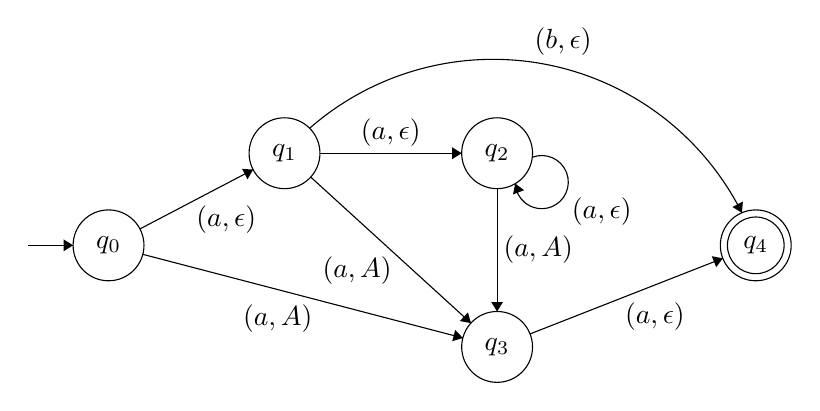
\begin{tikzpicture}[scale=0.15]
					\tikzstyle{every node}+=[inner sep=0pt]
					\draw [black] (44.8,-39.6) circle (3);
					\draw (44.8,-39.6) node {$q_3$};
					\draw [black] (44.8,-23.2) circle (3);
					\draw (44.8,-23.2) node {$q_2$};
					\draw [black] (11.9,-31) circle (3);
					\draw (11.9,-31) node {$q_0$};
					\draw [black] (66.7,-31) circle (3);
					\draw (66.7,-31) node {$q_4$};
					\draw [black] (66.7,-31) circle (2.4);
					\draw [black] (26.8,-23.2) circle (3);
					\draw (26.8,-23.2) node {$q_1$};
					\draw [black] (29.02,-25.22) -- (42.58,-37.58);
					\fill [black] (42.58,-37.58) -- (42.33,-36.67) -- (41.65,-37.41);
					\draw (32.95,-31.89) node [below] {$(a,A)$};
					\draw [black] (44.8,-26.2) -- (44.8,-36.6);
					\fill [black] (44.8,-36.6) -- (45.3,-35.8) -- (44.3,-35.8);
					\draw (45.3,-31.4) node [right] {$(a,A)$};
					\draw [black] (14.8,-31.76) -- (41.9,-38.84);
					\fill [black] (41.9,-38.84) -- (41.25,-38.16) -- (41,-39.12);
					\draw (26.22,-35.98) node [below] {$(a,A)$};
					\draw [black] (14.56,-29.61) -- (24.14,-24.59);
					\fill [black] (24.14,-24.59) -- (23.2,-24.52) -- (23.67,-25.41);
					\draw (21.87,-27.61) node [below] {$(a,\epsilon)$};
					\draw [black] (29.8,-23.2) -- (41.8,-23.2);
					\fill [black] (41.8,-23.2) -- (41,-22.7) -- (41,-23.7);
					\draw (35.8,-22.7) node [above] {$(a,\epsilon)$};
					\draw [black] (28.926,-21.086) arc (131.19389:26.68374:23.581);
					\fill [black] (65.53,-28.24) -- (65.61,-27.3) -- (64.72,-27.75);
					\draw (50.39,-14.96) node [above] {$(b,\epsilon)$};
					\draw [black] (47.768,-23.545) arc (111.09476:-176.90524:2.25);
					\draw (51.09,-28.18) node [right] {$(a,\epsilon)$};
					\fill [black] (46.33,-25.77) -- (46.15,-26.69) -- (47.09,-26.33);
					\draw [black] (47.59,-38.5) -- (63.91,-32.1);
					\fill [black] (63.91,-32.1) -- (62.98,-31.92) -- (63.35,-32.85);
					\draw (58.16,-35.85) node [below] {$(a,\epsilon)$};
					\draw [black] (5.1,-31) -- (8.9,-31);
					\fill [black] (8.9,-31) -- (8.1,-30.5) -- (8.1,-31.5);
				\end{tikzpicture}
			\end{center}
			\caption{ A \emph{simple} real-time transducer representing the regular function $\{(a,\epsilon)\}^*\{(aa,A)\}\cup \{(ab, \epsilon)\}$. }
			\label{fig:ex:FSR:T}
		\end{figure}
	
		\begin{figure}
			\begin{center}
				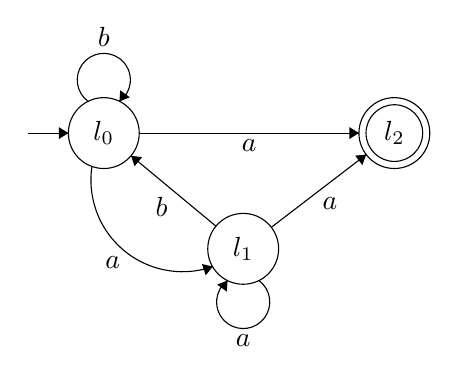
\begin{tikzpicture}[scale=0.15]
					\tikzstyle{every node}+=[inner sep=0pt]
					\draw [black] (27.3,-41.7) circle (3);
					\draw (27.3,-41.7) node {$l_1$};
					\draw [black] (15.5,-31.9) circle (3);
					\draw (15.5,-31.9) node {$l_0$};
					\draw [black] (40.1,-31.9) circle (3);
					\draw (40.1,-31.9) node {$l_2$};
					\draw [black] (40.1,-31.9) circle (2.4);
					\draw [black] (28.623,-44.38) arc (54:-234:2.25);
					\draw (27.3,-48.95) node [below] {$a$};
					\fill [black] (25.98,-44.38) -- (25.1,-44.73) -- (25.91,-45.32);
					\draw [black] (24.99,-39.78) -- (17.81,-33.82);
					\fill [black] (17.81,-33.82) -- (18.1,-34.71) -- (18.74,-33.94);
					\draw (20.39,-37.29) node [below] {$b$};
					\draw [black] (29.68,-39.88) -- (37.72,-33.72);
					\fill [black] (37.72,-33.72) -- (36.78,-33.81) -- (37.39,-34.61);
					\draw (34.65,-37.3) node [below] {$a$};
					\draw [black] (24.726,-43.204) arc (-70.78489:-188.63494:7.764);
					\fill [black] (24.73,-43.2) -- (23.81,-42.99) -- (24.13,-43.94);
					\draw (16.26,-42.34) node [below] {$a$};
					\draw [black] (14.177,-29.22) arc (234:-54:2.25);
					\draw (15.5,-24.65) node [above] {$b$};
					\fill [black] (16.82,-29.22) -- (17.7,-28.87) -- (16.89,-28.28);
					\draw [black] (18.5,-31.9) -- (37.1,-31.9);
					\fill [black] (37.1,-31.9) -- (36.3,-31.4) -- (36.3,-32.4);
					\draw (27.8,-32.4) node [below] {$a$};
					\draw [black] (9.1,-31.9) -- (12.5,-31.9);
					\fill [black] (12.5,-31.9) -- (11.7,-31.4) -- (11.7,-32.4);
				\end{tikzpicture}
			\end{center}
			\caption{ A \emph{right-simple} NFA representing the language $\{a,b\}^*\cdot\{a\}$. }
			\label{fig:ex:FSR:A_lambda}
		\end{figure}

		\begin{figure}
			\begin{center}
				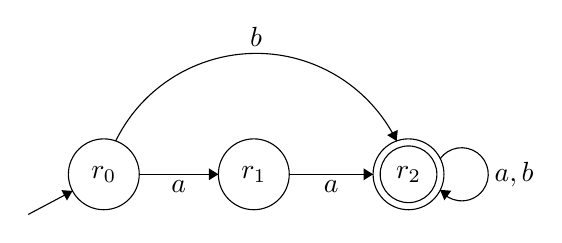
\begin{tikzpicture}[scale=0.15]
					\tikzstyle{every node}+=[inner sep=0pt]
					\draw [black] (18.4,-30) circle (3);
					\draw (18.4,-30) node {$r_0$};
					\draw [black] (44.2,-30) circle (3);
					\draw (44.2,-30) node {$r_2$};
					\draw [black] (44.2,-30) circle (2.4);
					\draw [black] (31.1,-30) circle (3);
					\draw (31.1,-30) node {$r_1$};
					\draw [black] (19.406,-27.18) arc (153.88499:26.11501:13.247);
					\fill [black] (43.19,-27.18) -- (43.29,-26.24) -- (42.39,-26.68);
					\draw (31.3,-19.26) node [above] {$b$};
					\draw [black] (21.4,-30) -- (28.1,-30);
					\fill [black] (28.1,-30) -- (27.3,-29.5) -- (27.3,-30.5);
					\draw (24.75,-30.5) node [below] {$a$};
					\draw [black] (34.1,-30) -- (41.2,-30);
					\fill [black] (41.2,-30) -- (40.4,-29.5) -- (40.4,-30.5);
					\draw (37.65,-30.5) node [below] {$a$};
					\draw [black] (46.88,-28.677) arc (144:-144:2.25);
					\draw (51.45,-30) node [right] {$a,b$};
					\fill [black] (46.88,-31.32) -- (47.23,-32.2) -- (47.82,-31.39);
					\draw [black] (12,-33.4) -- (15.75,-31.41);
					\fill [black] (15.75,-31.41) -- (14.81,-31.34) -- (15.28,-32.22);
				\end{tikzpicture}
			\end{center}
			\caption{ A \emph{left-simple} NFA representing the language $\{aa, b\}\cdot\{a,b\}^*$. }
			\label{fig:ex:FSR:A_rho}
		\end{figure}
	\end{example}
	
	\begin{construction} \label{constr:NFA_union}
		Let, for each $1\le r\le m$, $A_r = (\Sigma, Q_r, S_r, F_r, \Delta_r)$ be a NFA such that for $i\ne j$, $Q_i \cap Q_j = \emptyset$.
		Let $A$ be constructed as follows:
		\[ A \coloneq \left( \Sigma, \bigcup_{r=1}^m Q_r, \bigcup_{r=1}^m S_r, \bigcup_{r=1}^m F_r, \bigcup_{r=1}^m \Delta_r \right). \]
	\end{construction}
	\begin{proposition} \label{prop:constr:NFA_union}
		Let, for each $1\le r\le m$, $A_r = (\Sigma, Q_r, S_r, F_r, \Delta_r)$ be a NFA such that for $i\ne j$, $Q_i \cap Q_j = \emptyset$.
		Let A be obtained from construction~\ref{constr:NFA_union} applied on the sequence $(A_r)_{r=1}^{m}$.
		Then $\Lang(A) = \bigcup_{r=1}^m\Lang(A_r)$.
	\end{proposition}

	\begin{construction} \label{constr:NFA_concat_right}
		Let $A_1 = (\Sigma, Q_1, S_1, \{f_1\}, \Delta_1)$ and $A_2 = (\Sigma, Q_2, \{s_2\}, F_2, \Delta_2)$ be NFA such that $Q_1\cap Q_2 = \emptyset$.
		An NFA $A \coloneq (\Sigma, Q_1\cup Q_2, S_1, F, \Delta)$ is constructed where:
		\begin{itemize}
			\item \( F \coloneq F_2\cup
			\begin{cases}
				\emptyset & s_2\notin F_2 \\
				\{f_1\} & s_2\in F_2
			\end{cases}
			\),
			\item \( \Delta \coloneq \Delta_1\cup \Delta_2\cup \{ (f_1, a, q)\mid (s_2, a, q)\in \Delta_2 \} \).
		\end{itemize}
	\end{construction}
	\begin{proposition} \label{prop:constr:NFA_concat_right}
		Let $A_1 = (\Sigma, Q_1, S_1, \{f_1\}, \Delta_1)$ and $A_2 = (\Sigma, Q_2, \{s_2\}, F_2, \Delta_2)$ be NFA such that $Q_1\cap Q_2 = \emptyset$. Let $A$ be obtained from construction~\ref{constr:NFA_concat_right} applied on $A_1$ and $A_2$.
		Then $\Lang(A) = \Lang(A_1)\cdot\Lang(A_2)$.
	\end{proposition}
\iffalse
	\begin{construction} \label{constr:NFA_concat_left}
		Let $A_1 = (\Sigma, Q_1, S_1, \{f_1\}, \Delta_1)$ and $A_2 = (\Sigma, Q_2, \{s_2\}, F_2, \Delta_2)$ be NFA such that $Q_1\cap Q_2 = \emptyset$. We construct a NFA $A = (\Sigma, Q_1\cup Q_2, S, F_2, \Delta)$ where:
		\begin{itemize}
			\item \( S = S_1\cup
			\begin{cases}
				\emptyset & f_1\notin S_1 \\
				\{s_2\} & f_1\in S_1
			\end{cases}
			\),
			\item \( \Delta = \Delta_1\cup \Delta_2\cup \{ (q, a, s_2)\mid (q, a, f_1)\in \Delta_1 \} \).
		\end{itemize}
	\end{construction}
	Clearly, in both constructions~(\ref{constr:NFA_concat_right} and \ref{constr:NFA_concat_left}), $\Lang(A) = \Lang(A_1)\cdot\Lang(A_2)$.
\fi

	\section{Two-step bimachines} \label{section:TSBM}
	\begin{definition} \label{def:two-step_bimachine}
		We say that $A=(\Sigma_1, \Sigma_2, A_L, A_R, Q, q_0, \delta, \tau, \psi_\delta, \psi_\tau)$ is a two-step bimachine where:
		\begin{itemize}
			\item $\Sigma_1$ is a finite set called input alphabet,
			\item $\Sigma_2$ is a finite set called output alphabet,
			\item $Q$ is a finite set of states,
			\item $A_L=(\Sigma_1, Q_L, s_L, Q_L, \delta_L)$ is a DFA - the left automaton,
			\item $A_R=(\Sigma_1, Q_R, s_R, Q_R, \delta_R)$ is a DFA - the right automaton,
			\item $q_0\in Q$ is the initial state,
			\item $\delta: Q\times \Sigma_1\times Q_R \pfun Q$,
			\item $\tau: Q\times Q_L\times Q_R \pfun Q$,
			\item $\psi_\delta: Q\times \Sigma_1\times Q_R \pfun \Sigma_1\cup\Sigma_2^*$,
			\item $\psi_\tau: Q\times Q_L\times Q_R \pfun \Sigma_2^*$.
		\end{itemize}
	\end{definition}

	\begin{definition} \label{def:two-step_bimachine_exec}
		Let $A=(\Sigma_1, \Sigma_2, A_L, A_R, Q, q_0, \delta, \tau, \psi_\delta, \psi_\tau)$ be a two-step bimachine.
		Let $t=t_1\ldots t_n\in \Sigma_1^*$.
		Let $L_0, \ldots, L_n$ be the execution of $A_L$ over $t$ and
		$R_n, \ldots, R_0$ be the execution of $A_R$ over $\rev(t)$.
		Execution of $A$ over $t$ is the sequence $((L_i, q_i, \overline{q_i}, R_i, o_i, \overline{o_i}))_{i=0}^n$ where:
		\begin{itemize}
			\item \( \overline{q_i} = \tau(q_i, L_i, R_i), \quad 0\le i\le n \),
			\item \( q_i = \delta(\overline{q_{i-1}}, t_i, R_i), \quad 0 < i\le n \),
			\item \( o_0 = \epsilon \),
			\item \( \overline{o_i} = \psi_\tau(q_i, L_i, R_i), \quad 0\le i\le n \),
			\item \( o_i = \psi_\delta(\overline{q_{i-1}}, t_i, R_i), \quad 0 < i\le n \).
		\end{itemize}
		Output of $A$ for $t$ is $\mathrm{Out}_A(t)=o_0\overline{o_0}\ldots o_n\overline{o_n}$.
	\end{definition}

	\begin{construction} \label{constr:two-step_bimachine}
		Let \bcrr{m} be a BCRR over $(\Sigma_1, \Sigma_2)$.
		Let $((\mathcal{T}_r, \mathcal{E}_r, A_{\lambda_r}, A_{\rho_r}))_{r=1}^m$ be a FSR of \bcrr{m} (the input for the construction).
		
		Let $A_\lambda = (\Sigma_1, Q_{\lambda}, S_{\lambda}, F_{\lambda}, \Delta_{\lambda})$ be obtained from construction~\ref{constr:NFA_union} applied on $(A_{\lambda_r})_{r=1}^m$.
		The left automaton $A_L = (\Sigma_1, Q_L, s_L, Q_L, \delta_L)$ is obtained by applying a determinization procedure on $A_\lambda$, i.e.
		\begin{itemize}
			\item \( Q_L \subseteq \mathcal{P}(Q_\lambda) \),
			\item \( s_L \coloneq S_\lambda \),
			\item \( \delta_L(L, a) \coloneq \mathrm{Succ}_{A_\lambda}(L, a) \),\quad for $L\in Q_L$ and $a\in \Sigma_1$.
		\end{itemize}

		Let $\mathcal{T}_r^\mathrm{dom} = (\Sigma_1, Q_{T_r}, \{ s_{T_r} \}, \{ f_{T_r} \}, \Delta_{T_r}^{\Sigma_1})$ be the underlying automaton of $\mathcal{T}_r$.
		Let $\mathcal{T}^\mathrm{dom} = (\Sigma_1, Q_T, S_T, F_T, \Delta_T^{\Sigma_1})$ be obtained from construction~\ref{constr:NFA_union} applied on $(\mathcal{T}_r^\mathrm{dom})_{r=1}^m$. 
		Let	$\Delta_T = \bigcup_{r=1}^m \Delta_{T_r}$.
		For each $1\le r\le m$, let $A_{R_r} = (\Sigma_1, Q_{R_r}, S_{R_r}, F_{R_r}, \Delta_{R_r})$ be obtained from construction~\ref{constr:NFA_concat_right} applied on $\mathcal{T}_r^\mathrm{dom}$ and $A_{\rho_r}$.
		
		Now, let $A_{RU} = (\Sigma_1, Q_{RU}, S_{RU}, F_{RU}, \Delta_{RU})$ be obtained from construction~\ref{constr:NFA_union} applied on $(A_{R_r}^\mathrm{rev})_{r=1}^m$.
		Let $\mathrm{type} = \{ (q, r) \mid q\in Q_{T_r} \}$.
		Since $Q_{T_r} \cap Q_{T_{r'}} = \emptyset$ for $r\ne r'$, $\mathrm{type}: Q_T\to \{1,\ldots, m\}$ is a function.
		For $q\in Q_T$, we will say that $\mathrm{type}(q)$ is the type of $q$.
		The right automaton is $A_R = (\Sigma_1, Q_R, s_R, Q_R, \delta_R)$ where:
		\begin{itemize}
			\item \( \displaystyle Q_R \subseteq \mathcal{P}(Q_{RU}) \times
				\bigcup_{Q\subseteq Q_T} \mathrm{Enum}(Q)
			\),
			\item \( s_R \coloneq (S_{RU}, g_s) \),\quad where
				\begin{itemize}
					\item \( g_s\in \mathrm{Enum}(S_{RU} \cap F_T), \)
					\item \( (\forall i\in \Dom(g_s))(\forall j\in \Dom(g_s))(i\le j \implies
					\mathrm{type}(g_s(i))\le \mathrm{type}(g_s(j)) \),
				\end{itemize}
			\item \( \delta_R((R', g'), a) \coloneq (R, g) \),\quad for $(R', g')\in Q_R$ and $a\in \Sigma_1$ where $(R,g)$ is an arbitrary element with the following properties:
			\begin{itemize}
				\item \( R = \mathrm{Succ}_{A_{RU}}(R', a) \),
				\item \( g\in \mathrm{Enum}(R \cap Q_T), \)
				\item \( (\forall i\in \Dom(g))(\forall j\in \Dom(g))(i\le j \implies \\
					((g(i)\in F_T\ \&\ g(j)\in F_T\ \&\ \mathrm{type}(g(i))\le \mathrm{type}(g(j)))\ \lor\ \\
					(g(i)\notin F_T\ \&\ g(j)\in F_T)\ \lor\ \mu(g(i), a, g')\le \mu(g(j), a, g'))), \text{where} \\
					\mu(q, a, g') = \min\{ i' \mid (q, a, g'(i'))\in \Delta_T^{\Sigma_1} \} 
				\).
			\end{itemize}
		\end{itemize}
		
		Let $L\in Q_L$, $(R,g)\in Q_R$.
		We will define the following functions:
		\begin{eqnarray*}
			I(L, g)&\coloneq& \{ i \mid g(i)\in S_T\ \&\ f_{\lambda_{\mathrm{type}(g(i))}}\in L \}, \\
			\nu(L, g)&\coloneq& g(\min(I(L, g))), \\
			J(L, R)&\coloneq& \{ r \mid \mathcal{E}_r\downarrow\ \&\ f_{\lambda_r}\in L\ \&\ f_{T_r}\in R \}.
		\end{eqnarray*}

		The output of this construction is a two-step bimachine $A=(\Sigma_1, \Sigma_2, A_L, A_R, Q, q_\mathrm{err}, \delta, \tau, \psi_\delta, \psi_\tau)$ where:
		\begin{itemize}
			\item \( Q = Q_T \cup \{ q_\mathrm{err} \}, q_\mathrm{err}\notin Q_T \),
			\item \( \delta(\overline{q}, a, (R', g')) \coloneq
			\begin{cases}
				g'(\mu(\overline{q}, a, g')) & \overline{q}\in \Rng(g)\setminus F_T,\text{ where }(R, g) = \delta_R((R', g'), a) \\
				q_\mathrm{err} & \text{otherwise}
			\end{cases}
			\),
			\item \( \tau(q, L, (R, g)) \coloneq
			\begin{cases}
				q & q\in Q_T \setminus F_T \\
				\nu(L, g) & q\notin Q_T \setminus F_T\ \&\ I(L, g)\ne \emptyset \\
				q_\mathrm{err} & \text{otherwise}
			\end{cases}
			\),
			\item \( \psi_\delta(\overline{q}, a, (R', g')) \coloneq
			\begin{cases}
				\mathrm{elem\_of}\{ m \mid (\overline{q}, (a, m), \delta(\overline{q}, a, (R', g')))\in \Delta_T \} & \delta(\overline{q}, a, (R', g'))\in Q_T \\
				a & \text{otherwise}
			\end{cases}
			\),
			\item \( \psi_\tau(q, L, (R, g)) \coloneq
			\begin{cases}
				\mathcal{E}_{\min(J(L, R))} & \tau(q, L, (R, g)) = q_\mathrm{err}\ \&\ J(L, R)\ne \emptyset \\
				\epsilon & \text{otherwise}
			\end{cases}
			\).
		\end{itemize}
	\end{construction}

	\begin{example} \label{ex:two-step_bimachine}
		A possible result of applying construction~\ref{constr:two-step_bimachine} on the FSR $\langle (\mathcal{T}_1, \mathcal{E}_1, A_{\lambda_1}, A_{\rho_1}) \rangle$ from example~\ref{ex:FSR} is
		$\mathcal{A}=(\{a, b\}, \{A\}, A_L, A_R, Q, q_\mathrm{err}, \delta, \tau, \psi_\delta, \psi_\tau)$ where
		\begin{itemize}
			\item \( A_L = (\{a, b\}, Q_L, L_0, Q_L, \delta_L) \), where %\qquad (see figure~\ref{fig:ex:tsbm:A_L})
			\begin{itemize}
				\item \( Q_L = \{ L_0, L_1 \} \),
				\item \(
					\begin{aligned}
						L_0 &= \{l_0\} & \mathcolor{blue}{L_1 &= \{l_1, l_2\}} \\
					\end{aligned}
				\),
\iffalse
				\item \(
					\begin{aligned}
						\delta_L(L_0, a) &= L_1 & \delta_L(L_0, b) &= L_0 & \delta_L(L_1, a) &= L_1 & \delta_L(L_1, b) &= L_0 \\
					\end{aligned}
				\),
\fi
				\item For $\delta_L$ see figure~\ref{fig:ex:tsbm:A_L}.
			\end{itemize}
			\item \( A_R = (\{a, b\}, Q_R, R_0, Q_R, \delta_R) \), where %\qquad (see figure~\ref{fig:ex:tsbm:A_R})
			\begin{itemize}
				\item \( Q_R = \{R_0, R_1, R_2, R_3, R_4, R_5, R_6, R_7, R_8, R_9, R_{10}\} \),
				\item \(
					\begin{aligned}
						R_0 &= (\{ r_2 \}, 			&&	\langle  \rangle) 	 & \mathcolor{red}{R_6    &= (\{ r_0, r_1, r_2, q_3, q_4 \}, && \langle q_3, q_4 \rangle)} \\
						R_1 &= (\{ r_1, r_2 \}, 	&&	\langle  \rangle) 	 & \mathcolor{violet}{R_7    &= (\{ r_0, r_1, r_2, q_0, q_1, q_2, q_4 \}, && \langle q_1, q_2, q_0, q_4 \rangle)} \\
						\mathcolor{red}{R_2 &= (\{ r_0, r_2, q_4 \}, 	&&	\langle q_4 \rangle)} & \mathcolor{blue}{R_8    &= (\{ r_1, r_2, q_0, q_3 \},	   && \langle q_0, q_3 \rangle)} \\
						\mathcolor{red}{R_3 &= (\{ r_0, r_1, r_2, q_4 \},&&	\langle q_4 \rangle)} & \mathcolor{violet}{R_9    &= (\{ r_0, r_1, r_2, q_0, q_1, q_2, q_3, q_4 \}, && \langle q_1, q_2, q_0, q_3, q_4 \rangle)} \\
						R_4 &= (\{ r_1, r_2, q_3 \},		&&	\langle q_3 \rangle) & \mathcolor{violet}{R_{10} &= (\{ r_0, r_1, r_2, q_0, q_1, q_2, q_3, q_4 \}, && \langle q_0, q_1, q_2, q_3, q_4 \rangle)} \\
						\mathcolor{red}{R_5 &= (\{ r_0, r_2, q_4 \},		&&	\langle q_4 \rangle)} \\
					\end{aligned}
				\),
\iffalse
				\item \(
					\begin{aligned}
						\delta_R(R_0, a) &= R_1 & \delta_R(R_3, a) &= R_6 & \delta_R(R_6, a) &= R_9    & \delta_R(R_9,    b) &= R_{10} \\
						\delta_R(R_0, b) &= R_2 & \delta_R(R_3, b) &= R_5 & \delta_R(R_6, b) &= R_5    & \delta_R(R_9,    a) &= R_5 \\
						\delta_R(R_1, a) &= R_3 & \delta_R(R_4, a) &= R_7 & \delta_R(R_7, a) &= R_{10} & \delta_R(R_{10}, a) &= R_{10} \\
						\delta_R(R_1, b) &= R_2 & \delta_R(R_4, b) &= R_2 & \delta_R(R_7, b) &= R_5    & \delta_R(R_{10}, a) &= R_5 \\
						\delta_R(R_2, a) &= R_4 & \delta_R(R_5, a) &= R_8 & \delta_R(R_8, a) &= R_7    \\
						\delta_R(R_2, b) &= R_5 & \delta_R(R_5, b) &= R_5 & \delta_R(R_8, b) &= R_2    \\
					\end{aligned}
				\),
\fi
				\item For $\delta_R$ see figure~\ref{fig:ex:tsbm:A_R}.
			\end{itemize}
			\item \( Q = \{ q_0, q_1, q_2, q_3, q_4, q_\mathrm{err} \} \),
			\item For $\delta$ and $\psi_\delta$ see table~\ref{table:ex:tsbm:delta,tau_delta}, for $\tau$ and $\psi_\tau$ -- table~\ref{table:ex:tsbm:tau}.
		\end{itemize}
	
		\begin{figure}
			\begin{center}
				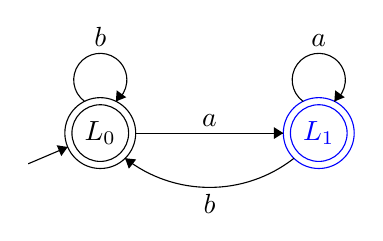
\begin{tikzpicture}[scale=0.15]
					\tikzstyle{every node}+=[inner sep=0pt]
					\draw [black] (12.1,-22.1) circle (3);
					\draw (12.1,-22.1) node {$L_0$};
					\draw [black] (12.1,-22.1) circle (2.4);
					\draw [blue] (30.6,-22.1) circle (3);
					\draw [blue] (30.6,-22.1) node {$L_1$};
					\draw [blue] (30.6,-22.1) circle (2.4);
					\draw [black] (6,-24.7) -- (9.34,-23.28);
					\fill [black] (9.34,-23.28) -- (8.41,-23.13) -- (8.8,-24.05);
					\draw [black] (15.1,-22.1) -- (27.6,-22.1);
					\fill [black] (27.6,-22.1) -- (26.8,-21.6) -- (26.8,-22.6);
					\draw (21.35,-21.6) node [above] {$a$};
					\draw [black] (29.277,-19.42) arc (234:-54:2.25);
					\draw (30.6,-14.85) node [above] {$a$};
					\fill [black] (31.92,-19.42) -- (32.8,-19.07) -- (31.99,-18.48);
					\draw [black] (10.777,-19.42) arc (234:-54:2.25);
					\draw (12.1,-14.85) node [above] {$b$};
					\fill [black] (13.42,-19.42) -- (14.3,-19.07) -- (13.49,-18.48);
					\draw [black] (28.502,-24.233) arc (-51.92771:-128.07229:11.599);
					\fill [black] (14.2,-24.23) -- (14.52,-25.12) -- (15.14,-24.33);
					\draw (21.35,-27.2) node [below] {$b$};
				\end{tikzpicture}
			\end{center}
			\caption{The left automaton of the two-step bimachine from example~\ref{ex:two-step_bimachine}. It lands on state $L_1$ (which contains the final state $l_2$ of $A_{\lambda_1}$) iff the last symbol read was $'a'$. This is used to determine whether a valid left context is present after reading some prefix of the input string.}
			\label{fig:ex:tsbm:A_L}
		\end{figure}
\iffalse
		\begin{figure}
			\begin{center}
				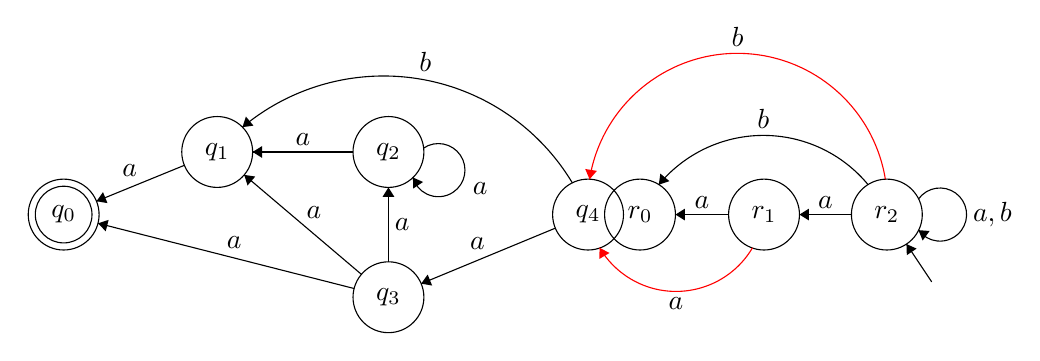
\begin{tikzpicture}[scale=0.15]
					\tikzstyle{every node}+=[inner sep=0pt]
					\draw [black] (53.2,-23.4) circle (3);
					\draw (53.2,-23.4) node {$r_0$};
					\draw [black] (63.7,-23.4) circle (3);
					\draw (63.7,-23.4) node {$r_1$};
					\draw (74.1,-23.4) circle (3);
					\draw (74.1,-23.4) node {$r_2$};
					\draw [black] (48.8,-23.4) circle (3);
					\draw (48.8,-23.4) node {$q_4$};
					\draw [black] (4.4,-23.4) circle (3);
					\draw (4.4,-23.4) node {$q_0$};
					\draw [black] (4.4,-23.4) circle (2.4);
					\draw [black] (17.4,-18.1) circle (3);
					\draw (17.4,-18.1) node {$q_1$};
					\draw [black] (31.9,-18.1) circle (3);
					\draw (31.9,-18.1) node {$q_2$};
					\draw [black] (31.9,-30.4) circle (3);
					\draw (31.9,-30.4) node {$q_3$};
					\draw [black] (76.78,-22.077) arc (144:-144:2.25);
					\draw (81.35,-23.4) node [right] {$a,b$};
					\fill [black] (76.78,-24.72) -- (77.13,-25.6) -- (77.72,-24.79);
					\draw [black] (71.1,-23.4) -- (66.7,-23.4);
					\fill [black] (66.7,-23.4) -- (67.5,-23.9) -- (67.5,-22.9);
					\draw (68.9,-22.9) node [above] {$a$};
					\draw [black] (60.7,-23.4) -- (56.2,-23.4);
					\fill [black] (56.2,-23.4) -- (57,-23.9) -- (57,-22.9);
					\draw (58.45,-22.9) node [above] {$a$};
					\draw [black] (54.791,-20.866) arc (140.40293:39.59707:11.497);
					\fill [black] (54.79,-20.87) -- (55.69,-20.57) -- (54.92,-19.93);
					\draw (63.65,-16.2) node [above] {$b$};
					\draw [black] (77.9,-29.1) -- (75.76,-25.9);
					\fill [black] (75.76,-25.9) -- (75.79,-26.84) -- (76.62,-26.28);
					\draw [black] (46.03,-24.55) -- (34.67,-29.25);
					\fill [black] (34.67,-29.25) -- (35.6,-29.41) -- (35.22,-28.48);
					\draw (39.44,-26.39) node [above] {$a$};
					\draw [black] (19.538,-16) arc (129.869:30.96972:18.64);
					\fill [black] (19.54,-16) -- (20.47,-15.87) -- (19.83,-15.1);
					\draw (35.03,-11.33) node [above] {$b$};
					\draw [black] (34.87,-17.773) arc (124.01689:-163.98311:2.25);
					\draw (39,-21.19) node [right] {$a$};
					\fill [black] (33.97,-20.26) -- (34,-21.2) -- (34.83,-20.64);
					\draw [black] (28.9,-18.1) -- (20.4,-18.1);
					\fill [black] (20.4,-18.1) -- (21.2,-18.6) -- (21.2,-17.6);
					\draw (24.65,-17.6) node [above] {$a$};
					\draw [black] (29.61,-28.46) -- (19.69,-20.04);
					\fill [black] (19.69,-20.04) -- (19.97,-20.94) -- (20.62,-20.18);
					\draw (25.6,-23.76) node [above] {$a$};
					\draw [black] (14.62,-19.23) -- (7.18,-22.27);
					\fill [black] (7.18,-22.27) -- (8.11,-22.43) -- (7.73,-21.5);
					\draw (9.99,-20.23) node [above] {$a$};
					\draw [black] (28.99,-29.66) -- (7.31,-24.14);
					\fill [black] (7.31,-24.14) -- (7.96,-24.82) -- (8.21,-23.85);
					\draw (18.84,-26.34) node [above] {$a$};
					\draw [black] (31.9,-27.4) -- (31.9,-21.1);
					\fill [black] (31.9,-21.1) -- (31.4,-21.9) -- (32.4,-21.9);
					\draw (32.4,-24.25) node [right] {$a$};
					\draw [red] (48.926,-20.41) arc (-189.19248:-350.80752:12.687);
					\fill [red] (48.93,-20.41) -- (49.55,-19.7) -- (48.56,-19.54);
					\draw (61.45,-9.25) node [above] {$b$};
					\draw [red] (62.722,-26.215) arc (-30.58353:-149.41647:7.518);
					\fill [red] (49.78,-26.22) -- (49.75,-27.16) -- (50.62,-26.65);
					\draw (56.25,-30.41) node [below] {$a$};
				\end{tikzpicture}
			\end{center}
			\caption{The automaton $A_{RU}$ obtained by reversing the concatenation (construction~\ref{constr:NFA_concat_right}) of $\mathcal{T}_1$ and $A_{\rho_1}$ from example~\ref{ex:FSR}. Note that, while reading the input string from right to left, it lands (nondeterministically) on $q_4$ iff a (reversed) valid right context has just been encountered (an empty match may begin). It lands (nondeterministically) on $q_0$ iff a (reversed) valid right context followed by a (reversed) string belonging to $\Dom(\mathcal{T}_1)$ has just been encountered (a non-empty match may begin).}
			\label{fig:ex:tsbm:A_{RU}}
		\end{figure}
\fi
		\begin{figure}
			\begin{center}
				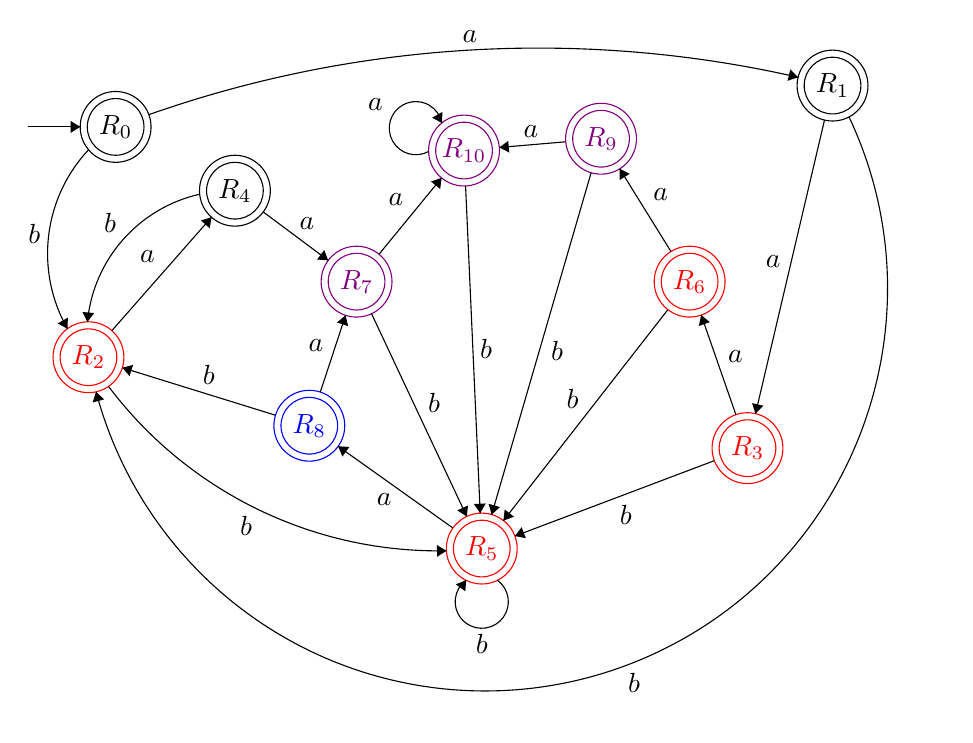
\begin{tikzpicture}[scale=0.15]
					\tikzstyle{every node}+=[inner sep=0pt]
					\draw [black] (13.6,-10.7) circle (3);
					\draw (13.6,-10.7) node {$R_0$};
					\draw [black] (13.6,-10.7) circle (2.4);
					\draw [black] (74.3,-7.2) circle (3);
					\draw (74.3,-7.2) node {$R_1$};
					\draw [black] (74.3,-7.2) circle (2.4);
					\draw [red] (44.6,-46.4) circle (3);
					\draw [red] (44.6,-46.4) node {$R_5$};
					\draw [red] (44.6,-46.4) circle (2.4);
					\draw [red] (11.3,-30.2) circle (3);
					\draw [red] (11.3,-30.2) node {$R_2$};
					\draw [red] (11.3,-30.2) circle (2.4);
					\draw [red] (67.1,-37.9) circle (3);
					\draw [red] (67.1,-37.9) node {$R_3$};
					\draw [red] (67.1,-37.9) circle (2.4);
					\draw [black] (23.7,-16.1) circle (3);
					\draw (23.7,-16.1) node {$R_4$};
					\draw [black] (23.7,-16.1) circle (2.4);
					\draw [violet] (34,-23.8) circle (3);
					\draw [violet] (34,-23.8) node {$R_7$};
					\draw [violet] (34,-23.8) circle (2.4);
					\draw [red] (62.2,-23.8) circle (3);
					\draw [red] (62.2,-23.8) node {$R_6$};
					\draw [red] (62.2,-23.8) circle (2.4);
					\draw [blue] (30,-36) circle (3);
					\draw [blue] (30,-36) node {$R_8$};
					\draw [blue] (30,-36) circle (2.4);
					\draw [violet] (54.7,-11.7) circle (3);
					\draw [violet] (54.7,-11.7) node {$R_9$};
					\draw [violet] (54.7,-11.7) circle (2.4);
					\draw [violet] (43.1,-12.7) circle (3);
					\draw [violet] (43.1,-12.7) node {$R_{10}$};
					\draw [violet] (43.1,-12.7) circle (2.4);
					\draw [black] (16.414,-9.661) arc (109.40682:77.19329:99.237);
					\fill [black] (71.39,-6.49) -- (70.72,-5.83) -- (70.49,-6.8);
					\draw (43.61,-3.64) node [above] {$a$};
					\draw [black] (9.525,-27.79) arc (-150.30302:-223.15074:12.855);
					\fill [black] (9.52,-27.79) -- (9.56,-26.85) -- (8.69,-27.34);
					\draw (7.26,-19.8) node [left] {$b$};
					\draw [black] (73.62,-10.12) -- (67.78,-34.98);
					\fill [black] (67.78,-34.98) -- (68.45,-34.31) -- (67.48,-34.09);
					\draw (69.94,-22.14) node [left] {$a$};
					\draw [black] (75.697,-9.854) arc (25.24312:-165.13093:34.075);
					\fill [black] (11.94,-33.13) -- (11.66,-34.03) -- (12.63,-33.77);
					\draw (57.49,-56.92) node [below] {$b$};
					\draw [black] (13.28,-27.95) -- (21.72,-18.35);
					\fill [black] (21.72,-18.35) -- (20.82,-18.62) -- (21.57,-19.28);
					\draw (16.96,-21.7) node [left] {$a$};
					\draw [black] (11.213,-27.209) arc (-185.35442:-257.30448:12.256);
					\fill [black] (11.21,-27.21) -- (11.79,-26.46) -- (10.79,-26.37);
					\draw (13.67,-18.81) node [left] {$b$};
					\draw [black] (41.607,-46.588) arc (-88.8645:-143.02009:34.944);
					\fill [black] (41.61,-46.59) -- (40.8,-46.1) -- (40.82,-47.1);
					\draw (24.64,-43.58) node [below] {$b$};
					\draw [black] (66.12,-35.07) -- (63.18,-26.63);
					\fill [black] (63.18,-26.63) -- (62.98,-27.55) -- (63.92,-27.23);
					\draw (65.41,-30.11) node [right] {$a$};
					\draw [black] (64.29,-38.96) -- (47.41,-45.34);
					\fill [black] (47.41,-45.34) -- (48.33,-45.52) -- (47.98,-44.59);
					\draw (56.79,-42.67) node [below] {$b$};
					\draw [black] (26.1,-17.9) -- (31.6,-22);
					\fill [black] (31.6,-22) -- (31.26,-21.12) -- (30.66,-21.93);
					\draw (29.8,-19.45) node [above] {$a$};
					\draw [black] (42.16,-44.66) -- (32.44,-37.74);
					\fill [black] (32.44,-37.74) -- (32.8,-38.61) -- (33.39,-37.8);
					\draw (36.35,-41.7) node [below] {$a$};
					\draw [black] (45.923,-49.08) arc (54:-234:2.25);
					\draw (44.6,-53.65) node [below] {$b$};
					\fill [black] (43.28,-49.08) -- (42.4,-49.43) -- (43.21,-50.02);
					\draw [black] (60.62,-21.25) -- (56.28,-14.25);
					\fill [black] (56.28,-14.25) -- (56.28,-15.19) -- (57.13,-14.67);
					\draw (59.08,-16.46) node [right] {$a$};
					\draw [black] (60.36,-26.17) -- (46.44,-44.03);
					\fill [black] (46.44,-44.03) -- (47.33,-43.71) -- (46.54,-43.09);
					\draw (52.83,-33.69) node [left] {$b$};
					\draw [black] (35.9,-21.48) -- (41.2,-15.02);
					\fill [black] (41.2,-15.02) -- (40.3,-15.32) -- (41.08,-15.96);
					\draw (37.99,-16.82) node [left] {$a$};
					\draw [black] (35.27,-26.52) -- (43.33,-43.68);
					\fill [black] (43.33,-43.68) -- (43.44,-42.75) -- (42.53,-43.17);
					\draw (40.01,-34.05) node [right] {$b$};
					\draw [black] (30.93,-33.15) -- (33.07,-26.65);
					\fill [black] (33.07,-26.65) -- (32.34,-27.26) -- (33.29,-27.57);
					\draw (31.23,-29.21) node [left] {$a$};
					\draw [black] (27.13,-35.11) -- (14.17,-31.09);
					\fill [black] (14.17,-31.09) -- (14.78,-31.8) -- (15.08,-30.85);
					\draw (21.5,-32.55) node [above] {$b$};
					\draw [black] (51.71,-11.96) -- (46.09,-12.44);
					\fill [black] (46.09,-12.44) -- (46.93,-12.87) -- (46.84,-11.88);
					\draw (48.76,-11.63) node [above] {$a$};
					\draw [black] (53.86,-14.58) -- (45.44,-43.52);
					\fill [black] (45.44,-43.52) -- (46.14,-42.89) -- (45.18,-42.61);
					\draw (50.42,-29.63) node [right] {$b$};
					\draw [black] (40.113,-12.772) arc (299.10445:11.10445:2.25);
					\draw (36.26,-8.82) node [left] {$a$};
					\fill [black] (41.23,-10.37) -- (41.27,-9.43) -- (40.4,-9.92);
					\draw [black] (43.23,-15.7) -- (44.47,-43.4);
					\fill [black] (44.47,-43.4) -- (44.93,-42.58) -- (43.93,-42.63);
					\draw (44.42,-29.53) node [right] {$b$};
					\draw [black] (6.2,-10.7) -- (10.6,-10.7);
					\fill [black] (10.6,-10.7) -- (9.8,-10.2) -- (9.8,-11.2);
				\end{tikzpicture}
			\end{center}
			\caption[]{
				The right automaton of the two-step bimachine from example~\ref{ex:two-step_bimachine}.
				The colors of the states are not part of the construction, their only purpose is to make the example easier to understand.
				If $t=\alpha\beta$, after reading $\beta$ from right to left, it lands on a state colored in
				\begin{itemize}
					\item \textcolor{red}{red} iff only an empty (but no non-empty) replacement may occur just after $\alpha$ (the enumeration part of red states contain $q_4$ and do not contain $q_0$),
					\item \textcolor{blue}{blue} iff only a non-empty (but no empty) replacement may occur just after $\alpha$ (the enumeration part of blue states contain $q_0$ and do not contain $q_4$),
					\item \textcolor{violet}{violet} iff both empty and non-empty replacement may occur just after $\alpha$ (the enumeration part of violet states contain both $q_0$ and $q_4$).
				\end{itemize}
				Note that in our construction, if after reading $\beta$ from right to left, the right automaton lands on a state colored in violet, an empty replacement will never occur just after $\alpha$ (non-empty replacements are longer than empty replacements).
			}
			\label{fig:ex:tsbm:A_R}
		\end{figure}
		
		\begin{table}[h!]
			\centering
			\begin{tabular}{c|c|c|c|c}
				$\overline{q}$ & $x$ & $R$ & $\delta(\overline{q}, x, R)$ & $\psi_\delta(\overline{q}, x, R)$ \\ \hline\hline
				$q_0$, $q_1$, $q_2$ & $a$ & $R_4$, $R_6$, $R_8$ & $q_3$ & $A$ \\ \hline
				$q_0$ & $a$ & $R_5$, $R_7$, $R_9$, $R_{10}$ & $q_1$ & $\epsilon$ \\ \hline
				$q_1$, $q_2$ & $a$ & $R_7$, $R_9$, $R_{10}$ & $q_2$ & $\epsilon$ \\ \hline
				$q_1$ & $b$ & $R_2$, $R_3$, $R_5$, $R_6$, $R_7$, $R_9$, $R_{10}$ & $q_4$ & $\epsilon$ \\ \hline
				$q_3$ & $a$ & $R_2$, $R_3$, $R_5$, $R_6$, $R_7$, $R_9$, $R_{10}$ & $q_4$ & $\epsilon$ \\
			\end{tabular}
			\caption{The functions $\delta$ and $\psi_\delta$ of $\mathcal{A}$ from example~\ref{ex:two-step_bimachine}.
				Unless otherwise specified, $\delta(\overline{q}, x, R) = q_\mathrm{err}$ and $\psi_\delta(\overline{q}, x, R) = x$.}
			\label{table:ex:tsbm:delta,tau_delta}
		\end{table}
		\begin{table}[h!]
			\centering
			\begin{tabular}{c|c|c|c|c}
				$q$ & $L$ & $R$ & $\tau(q, L, R)$ & $\psi_\tau(q, L, R)$ \\ \hline\hline
				$q_4$, $q_\mathrm{err}$ & $L_1$ & $R_7$, $R_8$, $R_9$, $R_{10}$ & $q_0$ & $\epsilon$ \\ \hline
				$q_0$ & any & any & $q_0$ & $\epsilon$ \\ \hline
				$q_1$ & any & any & $q_1$ & $\epsilon$ \\ \hline
				$q_2$ & any & any & $q_2$ & $\epsilon$ \\ \hline
				$q_3$ & any & any & $q_3$ & $\epsilon$ \\
			\end{tabular}
			\caption{The functions $\tau$ and $\psi_\tau$ of $\mathcal{A}$ from example~\ref{ex:two-step_bimachine}.
				Unless otherwise specified, $\tau(q, L, R) = q_\mathrm{err}$ and $\psi_\tau(q, L, R) = \epsilon$.}
			\label{table:ex:tsbm:tau}
		\end{table}
		The execution of $\mathcal{A}$ over the string $t=aaaaaabaaab$ is shown on figure~\ref{fig:ex:tsbm:execution}.
		\begin{figure}[h]
			\begin{adjustbox}{center=\textwidth}
			\setlength\tabcolsep{3pt} % default value: 6pt
			\begin{tabular}{*{23}{c}}
				$\mathcolor{violet}{R_{10}}$ &$\xleftarrow{a}$& $\mathcolor{violet}{R_{10}}$ &$\xleftarrow{a}$& $\mathcolor{violet}{R_{10}}$ &$\xleftarrow{a}$& $\mathcolor{violet}{R_{10}}$ &$\xleftarrow{a}$& $\mathcolor{violet}{R_7}$ &$\xleftarrow{a}$& $\mathcolor{blue}{R_8}$
				&$\xleftarrow{a}$& $\mathcolor{red}{R_5}$	&$\xleftarrow{b}$& $\mathcolor{violet}{R_{10}}$ &$\xleftarrow{a}$& $\mathcolor{violet}{R_7}$ &$\xleftarrow{a}$& $R_4$ &$\xleftarrow{a}$& $\mathcolor{red}{R_2}$
				&$\xleftarrow{b}$& $R_0$ \\
				$L_0$ &$\xrightarrow{a}$& $\mathcolor{blue}{L_1}$ &$\xrightarrow{a}$& $\mathcolor{blue}{L_1}$ &$\xrightarrow{a}$& $\mathcolor{blue}{L_1}$ &$\xrightarrow{a}$& $\mathcolor{blue}{L_1}$ &$\xrightarrow{a}$& $\mathcolor{blue}{L_1}$
				&$\xrightarrow{a}$& $\mathcolor{blue}{L_1}$ &$\xrightarrow{b}$& $L_0$ &$\xrightarrow{a}$& $\mathcolor{blue}{L_1}$ &$\xrightarrow{a}$& $\mathcolor{blue}{L_1}$ &$\xrightarrow{a}$& $\mathcolor{blue}{L_1}$
				&$\xrightarrow{b}$& $L_0$ \\
				\tikzmark{p0} && \tikzmark{p2} && \tikzmark{p4} && \tikzmark{p6} && \tikzmark{p8} && \tikzmark{p10} && \tikzmark{p12} && \tikzmark{p14} && \tikzmark{p16} && \tikzmark{p18} && \tikzmark{p20} && \tikzmark{p22} \\
				\multicolumn{23}{c}{\phantom{0}} \\
				\multicolumn{23}{c}{\phantom{0}} \\
				%0 &1& 2 && 2 && 3 && 4 && 5 && 6 && 7 && 8 && 9 && 10 && 11 \\
				\tikzmark{p1} && \tikzmark{p3} && \tikzmark{p5} && \tikzmark{p7} && \tikzmark{p9} && \tikzmark{p11} && \tikzmark{p13} && \tikzmark{p15} && \tikzmark{p17} && \tikzmark{p19} && \tikzmark{p21} && \tikzmark{p23} \\
			\end{tabular}
			\begin{tikzpicture}[overlay, remember picture]
				\node (P0) at ({pic cs:p0}) {$q_\mathrm{err}$};
				\node (P1) at ({pic cs:p1}) {$q_\mathrm{err}$};
				\node (P2) at ({pic cs:p2}) {$q_\mathrm{err}$};
				\node (P3) at ({pic cs:p3}) {$q_0$};
				\node (P4) at ({pic cs:p4}) {$q_1$};
				\node (P5) at ({pic cs:p5}) {$q_1$};
				\node (P6) at ({pic cs:p6}) {$q_2$};
				\node (P7) at ({pic cs:p7}) {$q_2$};
				\node (P8) at ({pic cs:p8}) {$q_2$};
				\node (P9) at ({pic cs:p9}) {$q_2$};
				\node (P10) at ({pic cs:p10}) {$q_3$};
				\node (P11) at ({pic cs:p11}) {$q_3$};
				\node (P12) at ({pic cs:p12}) {$q_4$};
				\node (P13) at ({pic cs:p13}) {$q_\mathrm{err}$};
				\node (P14) at ({pic cs:p14}) {$q_\mathrm{err}$};
				\node (P15) at ({pic cs:p15}) {$q_\mathrm{err}$};
				\node (P16) at ({pic cs:p16}) {$q_\mathrm{err}$};
				\node (P17) at ({pic cs:p17}) {$q_0$};
				\node (P18) at ({pic cs:p18}) {$q_3$};
				\node (P19) at ({pic cs:p19}) {$q_3$};
				\node (P20) at ({pic cs:p20}) {$q_4$};
				\node (P21) at ({pic cs:p21}) {$q_\mathrm{err}$};
				\node (P22) at ({pic cs:p22}) {$q_\mathrm{err}$};
				\node (P23) at ({pic cs:p23}) {$q_\mathrm{err}$};
				%\draw [->] ([yshift=5pt]{pic cs:0'}) -- ([yshift=-3pt]{pic cs:1'}) node[midway,left] {$\epsilon$};
				%\draw [->] ([yshift=5pt]{pic cs:1}) -- ([yshift=-5pt]{pic cs:2}) node[midway,above] {$a$};
				\draw [->] (P0) -- (P1) node[midway,left] {$\epsilon$};
				\draw [->] (P2) -- (P3) node[midway,left] {$\epsilon$};
				\draw [->] (P4) -- (P5) node[midway,left] {$\epsilon$};
				\draw [->] (P6) -- (P7) node[midway,left] {$\epsilon$};
				\draw [->] (P8) -- (P9) node[midway,left] {$\epsilon$};
				\draw [->] (P10) -- (P11) node[midway,left] {$\epsilon$};
				\draw [->] (P12) -- (P13) node[midway,left] {$\epsilon$};
				\draw [->] (P14) -- (P15) node[midway,left] {$\epsilon$};
				\draw [->] (P16) -- (P17) node[midway,left] {$\epsilon$};
				\draw [->] (P18) -- (P19) node[midway,left] {$\epsilon$};
				\draw [->] (P20) -- (P21) node[midway,left] {$\epsilon$};
				\draw [->] (P22) -- (P23) node[midway,left] {$\epsilon$};
				\draw [->] (P1) -- (P2) node[midway,above] {$a$} node[midway,below] {$a$};
				\draw [->] (P3) -- (P4) node[midway,above] {$a$} node[midway,below] {$\epsilon$};
				\draw [->] (P5) -- (P6) node[midway,above] {$a$} node[midway,below] {$\epsilon$};
				\draw [->] (P7) -- (P8) node[midway,above] {$a$} node[midway,below] {$\epsilon$};
				\draw [->] (P9) -- (P10) node[midway,above] {$a$} node[midway,below] {$A$};
				\draw [->] (P11) -- (P12) node[midway,above] {$a$} node[midway,below] {$\epsilon$};
				\draw [->] (P13) -- (P14) node[midway,above] {$b$} node[midway,below] {$b$};
				\draw [->] (P15) -- (P16) node[midway,above] {$a$} node[midway,below] {$a$};
				\draw [->] (P17) -- (P18) node[midway,above] {$a$} node[midway,below] {$A$};
				\draw [->] (P19) -- (P20) node[midway,above] {$a$} node[midway,below] {$\epsilon$};
				\draw [->] (P21) -- (P22) node[midway,above] {$b$} node[midway,below] {$b$};
			\end{tikzpicture}
			\end{adjustbox}
		\caption{The execution of $\mathcal{A}$ over $t=aaaaaabaaab$. $\mathrm{Out}_\mathcal{A}(t) = aAbaAb$.}
		\label{fig:ex:tsbm:execution}
		\end{figure}
\iffalse
		\begin{table}[h!]
		\centering
		\begin{adjustbox}{width=1.2\textwidth,center=\textwidth}
			%\small
			\begin{tabular}{c|c|c|p{130mm}}
				step & state & output & comment \\ \hline\hline
				0.1 & $q_\mathrm{err}$ & $\epsilon$ & The initial state. \\ \hline
				0.2 & $q_\mathrm{err}$ & $\epsilon$ &
					$\tau(q_\mathrm{err}, L_0, R_{10})=q_\mathrm{err}$; $\psi_\tau(q_\mathrm{err}, L_0, R_{10})=\epsilon$ \newline
				Cannot start a match - no valid left context. Since our rule does not allow empty replacements, the output at steps x.2 will always be $\epsilon$. \\ \hline
				1.1 & $q_\mathrm{err}$ & $a$ &
					$\delta(q_\mathrm{err}, a, R_{10}) = q_\mathrm{err}$; $\psi_\delta(q_\mathrm{err}, a, R_{10}) = a$ \newline
				Outside of match - $\psi_\delta$ just copies the input. \\ \hline
				1.2 & $q_0$ & $\epsilon$ & 
					$\tau(q_\mathrm{err}, L_1, R_{10})=q_0$; $\psi_\tau(q_\mathrm{err}, L_1, R_{10})=\epsilon$ \newline
				A left context is present ($l_2\in L_1$). A non-empty replacement is allowed to begin at that position ($R_{10}$ is colored in violet). The machine is currently not carrying out another replacement (the last state is $q_\mathrm{err}\notin Q_T\setminus F_T$). A non-empty match must begin (this ensures that the leftmost possible match will be rewritten). \\ \hline
				2.1 & $q_1$ & $\epsilon$ & 
					$\delta(q_0, a, R_{10}) = q_1$; $\psi_\delta(q_0, a, R_{10}) = \epsilon$ \newline
				The accessible states from $q_0$ with the symbol $'a'$ are $q_1$ and $q_3$. Among them, the state which has the least index in the enumeration part of $R_{10}$ is chosen (in this case $q_1$). This ensures that the longest possible match will be rewritten.
				The output of the corresponding transition is returned by $\psi_\delta$. Note that it is uniquely defined, since $\mathcal{T}_1$ represents a function. \\ \hline
				2.2 & $q_1$ & $\epsilon$ &
					$\tau(q_1, L_1, R_{10})=q_1$; $\psi_\tau(q_1, L_1, R_{10})=\epsilon$ \newline
				While a match is being processed, the function $\tau$ returns its first argument unchanged. This ensures that no overlapping matches will be rewritten. \\ \hline
				3.1 & $q_2$ & $\epsilon$ & 
					$\delta(q_1, a, R_{10}) = q_2$; $\psi_\delta(q_1, a, R_{10}) = \epsilon$ \\ \hline
				3.2 & $q_2$ & $\epsilon$ &
					$\tau(q_2, L_1, R_{10})=q_2$; $\psi_\tau(q_2, L_1, R_{10})=\epsilon$ \\ \hline
				4.1 & $q_2$ & $\epsilon$ & 
					$\delta(q_2, a, R_7) = q_2$; $\psi_\delta(q_2, a, R_7) = \epsilon$ \\ \hline
				4.2 & $q_2$ & $\epsilon$ & 
					$\tau(q_2, L_1, R_7)=q_2$; $\psi_\tau(q_2, L_1, R_7)=\epsilon$ \\ \hline
				5.1 & $q_3$ & $A$ & 
					$\delta(q_2, a, R_8) = q_3$; $\psi_\delta(q_2, a, R_8) = A$ \\ \hline
				5.2 & $q_3$ & $\epsilon$ & 
					$\tau(q_3, L_1, R_8)=q_3$; $\psi_\tau(q_3, L_1, R_8)=\epsilon$ \\ \hline
				6.1 & $q_4$ & $\epsilon$ & 
					$\delta(q_3, a, R_5) = q_4$; $\psi_\delta(q_3, a, R_5) = \epsilon$ \newline
					The machine reached the state $q_4\in F_T$ which means the current match has just finished. \\ \hline
				6.2 & $q_\mathrm{err}$ & $\epsilon$ & 
					$\tau(q_4, L_1, R_5)=q_\mathrm{err}$; $\psi_\tau(q_4, L_1, R_5)=\epsilon$ \newline
					A left context is present but no non-empty match can begin ($R_5$ is colored in red).
					Note however that the only reason an empty match is not rewritten at this step is that $\mathcal{E}_1$ is undefined (the rule does not allow rewriting the empty string). All other conditions for an empty match are satisfied. If $\mathcal{E}_1$ was defined, the output at this step would have been $\mathcal{E}_1$. \\ \hline
				7.1 & $q_\mathrm{err}$ & $b$ & 
					$\delta(q_\mathrm{err}, b, R_{10}) = q_\mathrm{err}$; $\psi_\delta(q_\mathrm{err}, b, R_{10}) = b$ \\ \hline
				7.2 & $q_\mathrm{err}$ & $\epsilon$ & 
					$\tau(q_\mathrm{err}, L_0, R_{10})=q_\mathrm{err}$; $\psi_\tau(q_\mathrm{err}, L_0, R_{10})=\epsilon$ \\ \hline
				8.1 & $q_\mathrm{err}$ & $a$ & 
					$\delta(q_\mathrm{err}, a, R_7) = q_\mathrm{err}$; $\psi_\delta(q_\mathrm{err}, a, R_7) = a$ \\ \hline
				8.2 & $q_0$ & $\epsilon$ & 
					$\tau(q_\mathrm{err}, L_1, R_7)=q_0$; $\psi_\tau(q_\mathrm{err}, L_1, R_7)=\epsilon$ \\ \hline
				9.1 & $q_3$ & $A$ & 
					$\delta(q_0, a, R_4) = q_3$; $\psi_\delta(q_0, a, R_4) = A$ \\ \hline
				9.2 & $q_3$ & $\epsilon$ & 
					$\tau(q_3, L_1, R_4)=q_3$; $\psi_\tau(q_3, L_1, R_4)=\epsilon$ \\ \hline
				10.1 & $q_4$ & $\epsilon$ & 
					$\delta(q_3, a, R_2) = q_4$; $\psi_\delta(q_3, a, R_2) = \epsilon$ \\ \hline
				10.2 & $q_\mathrm{err}$ & $\epsilon$ & 
					$\tau(q_4, L_1, R_2)=q_\mathrm{err}$; $\psi_\tau(q_4, L_1, R_2)=\epsilon$ \\ \hline
				11.1 & $q_\mathrm{err}$ & $b$ & 
					$\delta(q_\mathrm{err}, b, R_0) = q_\mathrm{err}$; $\psi_\delta(q_\mathrm{err}, b, R_0) = b$ \\ \hline
				11.2 & $q_\mathrm{err}$ & $\epsilon$ & 
					$\tau(q_\mathrm{err}, L_0, R_0)=q_\mathrm{err}$; $\psi_\tau(q_\mathrm{err}, L_0, R_0)=\epsilon$ \\
			\end{tabular}
		\end{adjustbox}
		\caption{Detailed description of the execution of $\mathcal{A}$ over the string $t=aaaaaabaaab$. The output of $\mathcal{A}$ over $t$ is the concatenation of the outputs at each step, namely $\mathrm{Out}_\mathcal{A}(t)=aAbaAb$.}
		\label{table:ex:tsbm:execution}
		\end{table}
\fi
	\end{example}

	\begin{proposition} \label{prop:construction_two-step_bimachine_correctness}
		Construction~\ref{constr:two-step_bimachine} correctly defines a two-step bimachine $A$.
	\end{proposition}
	\begin{proof}
		Clearly, $\tau$ and $\psi_\tau$ are correctly defined.
		For $g_s$, we just need to sort the states in $S_{RU}\cap F_T$ by their type.
		
		Let $(R', g')\in Q_R$, $a\in \Sigma_1$ and $R = \mathrm{Succ}_{A_{RU}}(R', a)$.
		We are going to show that there exists $g\in \mathrm{Enum}(R \cap Q_T)$ such that $(R, g)$ can be a value of $\delta_R((R', g'), a)$. For this purpose, we will define a sequence $(g_i)_{i=0}^{\len{g'}-1}$ where
		\begin{eqnarray*}
			g_0 & = & \mathrm{enumerate}(\{ q\mid (q, a, g'(0))\in\Delta_T^{\Sigma_1} \}), \\
			g_{i+1} & = & g_i\mathbin\Vert\mathrm{enumerate}(\{ q\mid (q, a, g'(i+1))\in\Delta_T^{\Sigma_1} \mathbin\& q\notin \Rng(g_i) \}).
		\end{eqnarray*}
		Note that the requirement $q\notin \Rng(g_i)$ ensures that $g_i$ and the new enumeration generated in step $i+1$ have no common elements in their range, so the concatenation is well-defined and therefore the whole sequence is well-defined. Let $g_\mathrm{old} = g_{\len{g'}-1}$.
		Let $g_\mathrm{new}$ be the enumeration of $R\cap F_T$ in which the states are sorted in ascending order by their type.
		$\Rng(g_\mathrm{old})\cap \Rng(g_\mathrm{new}) = \emptyset$ because, for each $1\le r\le m$, $\mathcal{T}_r$ is simple and in particular there are no transitions in $\Delta_T$ coming out of $f_{T_r}$ (so $\Rng(g_\mathrm{old})\cap F_T = \emptyset$). We claim that \[ g = g_\mathrm{old} \mathbin\Vert g_\mathrm{new} \] has the desired properties. Let $i\le j$.
		It is not possible that $g(i)\in F_T$ and $g(j)\notin F_T$.
		If $g(i), g(j)\in F_T$, then clearly $g(i), g(j)\in \Rng(g_\mathrm{new})$ and so $\mathrm{type}(g(i))\le \mathrm{type}(g(j))$ because the states in $g_\mathrm{new}$ are sorted in ascending order by their type.
		Now assume $g(i), g(j)\notin F_T$. Then $g(i), g(j)\in \Rng(g_\mathrm{old})$.
		Let $k_1 = \min\{k\mid g(i)\in \Rng(g_k)\}$ and $k_2 = \min\{k\mid g(j)\in \Rng(g_k)\}$. $i\le j$ implies that $k_1\le k_2$.
		By the definition of $k_1$, $(g(i), a, g'(k_1))\in \Delta_T^{\Sigma_1}$ and also $(\forall k<k_1)(g(i)\notin \Rng(g_k))$.
		Therefore $(\forall k<k_1)(g(i), a, g'(k))\notin \Delta_T^{\Sigma_1}$. This means $k_1 = \mu(g(i), a, g')$.
		Similarly, we can see that $k_2 = \mu(g(j), a, g')$.
		It remains to see that $g\in \mathrm{Enum}(R\cap Q_T)$, i.e.\ $\Rng(g) = R\cap Q_T$:
		\begin{description}
			\item[$\subseteq:$] Let $q\in \Rng(g)$. If $q\in \Rng(g_\mathrm{new})$, then $q\in(R\cap F_T)\subseteq(R\cap Q_T)$.
			Otherwise $q\in \Rng(g_\mathrm{old})$ and there is $q'\in \Rng(g') = R'\cap Q_T$ such that $(q, a, q')\in \Delta_T^{\Sigma_1}$. Therefore $q\in R\cap Q_T$.
			\item[$\supseteq:$] Let $q\in R\cap Q_T$. If $q\in F_T$, then $q\in\Rng(g_\mathrm{new})\subseteq\Rng(g)$.
			Assume $q\notin F_T$. Since $q\in R$, there is $q'\in R'$ such that $(q', a, q)\in \Delta_{RU}$. Since $q\in Q_T\setminus F_T$, it follows that $q'\in Q_T$ which means $(q, a, q')\in \Delta_T^{\Sigma_1}$ and hence $q'\in (R'\cap Q_T) = \Rng(g')$.
			Therefore $q\in \Rng(g_i)$ for some $0\le i < \len{g'}$. Thus $q\in \Rng(g_\mathrm{old})\subseteq \Rng(g)$.
		\end{description}
		With the above reasonings we have shown that $g$ has the desired properties and therefore the definition of $\delta_R$ is correct.
\iffalse
		\begin{algorithm}
			\caption{NextState($(R', g'), a$) computes $\delta_R((R', g'), a)$.}
			\label{alg:delta_R}
			\begin{multicols}{2}
				\begin{algorithmic}[1]
					\Function{NextSeq}{$R$, $g'$, $a$}
					\State $g\gets \langle\rangle$; $i=0$
					\For{$j\gets 0$ \textbf{to} $\len{g'}-1$}
					\For{$(q, a, g'[j])\in\Delta_T^{\Sigma_1}$}
					\If{$q\notin g[0..i-1]$}
					\State $g[i]\gets q$
					\State $i\gets i+1$
					\EndIf
					\EndFor
					\EndFor
					\For{$r\gets 1$ \textbf{to} $m$} \label{alg:delta_R:NextSeq:for_final_states}
					\If{$f_{T_r}\in R$}
					\State $g[i]\gets f_{T_r}$
					\State $i\gets i+1$
					\EndIf
					\EndFor
					\State \textbf{return} $g$
					\EndFunction
					\columnbreak
					\Function{NextState}{($R'$, $g'$), $a$}
					\State $R\gets \mathrm{Succ}_{A_{RU}}(R', a)$
					\State $g\gets$ \Call{NextSeq}{$R$, $g'$, $a$}
					\State \textbf{return} $(R, g)$
					\EndFunction
				\end{algorithmic}
			\end{multicols}
		\end{algorithm}
		Given $(R', g')\in Q_R$ and $a\in \Sigma_1$ we can obtain $(R, g)$ by calling NextState($(R', g'), a$) from algorithm~\ref{alg:delta_R}.
		Clearly, NextState($(R', g'), a$) eventually terminates. 
		Let $k$ be the value of the variable $i$ exactly before line~\ref{alg:delta_R:NextSeq:for_final_states} is reached for the first time. Then the following hold:
		\[
			(\forall i < k)(g(i)\notin F_T)\ \&\ 
			(\forall i\ge k)(i\in\Dom(g)\implies g(i)\in F_T).
		\]
		The first conjunct is true because, for each $1\le r\le m$, $\mathcal{T}_r$ is simple and in particular there are no transitions coming out of $f_{T_r}$. For the second conjunct, note that only final states are added to $g$ in the body of the "for" loop on line~\ref{alg:delta_R:NextSeq:for_final_states}.
		Let $i\le j$. It is not possible that $g(i)\in F_T$ and $g(j)\notin F_T$.
		If $g(i), g(j)\in F_T$, then clearly $\mathrm{type}(g(i))\le \mathrm{type}(g(j))$ because the final states are added in ascending order of their type.
		Now assume $g(i), g(j)\notin F_T$ and let $j_1$ be the value of the variable $j$ when $g(i)$ was added to $g$ and $j_2$ be the value of the variable $j$ when $g(j)$ was added to $g$ respectively. $g(i)$ was added to $g$ before $g(j)$ was, so $j_1\le j_2$.
		Since $g(i)$ was added to $g$ at step $j_1$ of the outer loop, we have $g(i)\notin g[0..i-1]$.
		Therefore, for all $j' < j_1$, $(g(i), a, g'(j'))\notin \Delta_T^{\Sigma_1}$ or otherwise $g(i)$ would not have been added to $g$ at step $j_1$ but on some earlier step. Thus $j_1 = \mu(g(i), a, g')$. Similarly, we can see that $j_2 = \mu(g(j), a, g')$.
		It is also clear that if $g'\in \mathrm{Enum}(R'\cap Q_T)$, then $g\in \mathrm{Enum}(R\cap Q_T)$, so g has the desired properties. Therefore the definition of $\delta_R$ is correct.
\fi

		For $\delta$, let $(R, g) = \delta_R((R', g'), a)$ and assume $\overline{q}\in \Rng(g)\setminus F_T$.
		Then $\overline{q}\in R = \mathrm{Succ}(R', a, \Delta_{RU})$ which means that there exists $q'\in R'$ such that $(q', a, \overline{q})\in \Delta_{RU}$.
		Since $\overline{q}\in \Rng(g)\setminus F_T$, we can conclude that $(q', a, \overline{q})\in {\left(\Delta_T^{\Sigma_1}\right)}^\mathrm{rev}$, i.e.\ $(\overline{q}, a, q')\in \Delta_T^{\Sigma_1}$.
		Therefore $q'\in (R'\cap Q_T) = \Rng(g')$, so $\{ i' \mid (\overline{q}, a, g'(i'))\in \Delta_T^{\Sigma_1} \}\ne \emptyset$.
		Hence $\mu(\overline{q}, a, g')$ is defined.
		All elements of $\{ i' \mid (\overline{q}, a, g'(i'))\in \Delta_T^{\Sigma_1} \}$ belong to the domain of $g'$ and in particular $\mu(\overline{q}, a, g')$ does.
		We can conclude that $g'(\mu(\overline{q}, a, g'))$ is defined and so is $\delta(\overline{q}, a, (R', g'))$.
		
		For $\psi_\delta$, let $q' = \delta(\overline{q}, a, (R', g'))$ and assume $q'\in Q_T$. Note that $q'\notin S_T$.
		We have that $(\overline{q}, a, q')\in \Delta_T^{\Sigma_1}$, so $\{ m \mid (\overline{q}, (a, m), q')\in \Delta_T \}\ne \emptyset$.
		Hence $\psi_\delta(\overline{q}, a, (R', g'))$ is correctly defined.
	\end{proof}

	Let $\mathrm{BR}=\bcrr{m}$ be a BCRR over $(\Sigma_1, \Sigma_2)$.
	Let $A=(\Sigma_1, \Sigma_2, A_L, A_R, Q, q_\mathrm{err}, \delta, \tau, \psi_\delta, \psi_\tau)$ be obtained from construction~\ref{constr:two-step_bimachine} applied on $((\mathcal{T}_r, \mathcal{E}_r, A_{\lambda_r}, A_{\rho_r}))_{r=1}^m$ -- a FSR of $\mathrm{BR}$.

	\begin{proposition} \label{prop:execution_is_correct}
		Let $t=t_1\ldots t_n\in \Sigma_1^*$ and $((L_i, q_i, \overline{q_i}, (R_i, g_i), o_i, \overline{o_i}))_{i=0}^n$ be an execution of $A$ over $t$. If $\overline{q_i}\in Q_T$, then $\overline{q_i}\in \Rng(g_i)\setminus F_T$.
	\end{proposition}
	\begin{proof}
		\begin{description}
			\item[$q_i\notin Q_T\setminus F_T:$]
				From $\overline{q_i}\ne q_\mathrm{err}$ it follows that $\overline{q_i}\in\Rng(g_i)$ and $\overline{q_i}\in S_T$.
				Since $S_T\cap F_T = \emptyset$, we have $\overline{q_i}\notin F_T$ and hence $\overline{q_i}\in\Rng(g_i)\setminus F_T$.
			\item[$q_i\in Q_T\setminus F_T:$]
				Recall that $q_0 = q_\mathrm{err}\notin Q_T$. Therefore $i > 0$. Then $q_i = \delta(\overline{q_{i-1}}, t_i, (R_i, g_i))\in\Rng(g_i)$. By definition, $\overline{q_i} = \tau(q_i, L_i, (R_i, g_i)) = q_i\in\Rng(g_i)$. Since $q_i\notin F_T$ and $\overline{q_i} = q_i$, it follows $\overline{q_i}\in \Rng(g_i)\setminus F_T$.
		\end{description}
	\end{proof}

	\begin{proposition} \label{prop:execution_last_state}
		Let $t=t_1\ldots t_n\in \Sigma_1^*$ and $((L_i, q_i, \overline{q_i}, (R_i, g_i), o_i, \overline{o_i}))_{i=0}^n$ be an execution of $A$ over $t$. Then $\overline{q_n} = q_\mathrm{err}$.
	\end{proposition}
	\begin{proof}
		Suppose $\overline{q_n}\ne q_\mathrm{err}$. Then $\overline{q_n}\in Q_T\setminus F_T$.
		\begin{description}
			\item[$\overline{q_n}\in S_T:$]
			Then $\overline{q_n}\in \Rng(g_n) = \Rng(g_s)\subseteq F_T$ - an immediate contradiction.
			\item[$\overline{q_n}\in Q_T\setminus (S_T\cup F_T):$]
			Then $\overline{q_n} = q_n\notin F_T$. But $q_n\in \Rng(g_n) = \Rng(g_s)\subseteq F_T$ - again a contradiction.
		\end{description}
	\end{proof}

	\begin{proposition} \label{prop:execution_left_right_DFA}
		Let $t=t_1\ldots t_n\in \Sigma_1^*$ and $((L_i, q_i, \overline{q_i}, (R_i, g_i), o_i, \overline{o_i}))_{i=0}^n$ be an execution of $A$ over $t$. Then, for each $0\le i\le n$,
		\begin{eqnarray*}
			f_{\lambda_r}\in L_i & \iff & t_1\ldots t_i\in \Sigma_1^*\cdot\lambda_r, \\
			s_{T_r}\in R_i & \iff & t_{i+1}\ldots t_n\in (\Dom(T_r)\setminus\{\epsilon\})\cdot\rho_r\cdot\Sigma_1^*, \\
			f_{T_r}\in R_i & \iff & t_{i+1}\ldots t_n\in \rho_r\cdot\Sigma_1^*.
		\end{eqnarray*}
	\end{proposition}

\iffalse
	\begin{proposition} \label{prop:execution_defined}
		Let $t=t_1\ldots t_n\in \Sigma_1^*$. Then the execution $((L_i, q_i, \overline{q_i}, (R_i, g_i), o_i, \overline{o_i}))_{i=0}^n$ of $A$ over $t$ is correctly defined.
	\end{proposition}
	\begin{proof}
		By induction on $i$:
		\begin{description}
			\item[$i=0:$]
			It is clear that $(L_0, q_0, \overline{q_0}, (R_0, g_0), o_0, \overline{o_0})$ is correctly defined.
			\item[$0<i\le n:$]
			It is clear that $L_i$ and $(R_i, g_i)$ are defined.
			Assume that $((L_j, q_j, \overline{q_j}, (R_j, g_j), o_j, \overline{o_j}))_{j=0}^{i-1}$ is correctly defined.
			We have \( q_i = \delta(\overline{q_{i-1}}, t_i, (R_i, g_i)) \). If $\overline{q_{i-1}}\notin Q_T$, then $q_i = q_\mathrm{err}$ is defined. Otherwise there are two cases:
			\begin{description}
				\item[$\overline{q_{i-1}}\in S_T:$]
				Then $\overline{q_{i-1}}$ is defined by the second case of the definition of $\tau$, so $\overline{q_{i-1}}\in \Rng(g_{i-1})$.
				\item[$\overline{q_{i-1}}\in Q_T\setminus S_T:$]
				Then $\overline{q_{i-1}}$ is defined by the first case of the definition of $\tau$, so $\overline{q_{i-1}} = q_{i-1} \in \Rng(g_{i-1})$.
			\end{description}
			In both cases $\overline{q_{i-1}}\in \Rng(g_{i-1})\subseteq R_{i-1}$, so there is a state $q'\in R_i$ such that $(q', t_i, \overline{q_{i-1}})\in \Delta_{RU}$. Note that $\tau$ never returns states in $F_T$. Therefore $\overline{q_{i-1}}\in Q_T\setminus F_T$ and hence $(q', t_i, \overline{q_{i-1}})\in {\left(\Delta_T^{\Sigma_1}\right)}^\mathrm{rev}$. Thus $q'\in Q_T$ which means $q'\in \Rng(g_i)$, so $\{ i' \mid (\overline{q_{i-1}}, t_i, g_i(i'))\in \Delta_T^{\Sigma_1} \}\ne \emptyset$. Therefore $q_i$ is correctly defined.
			
			With $q_i$ correctly defined, $\overline{q_i}, o_i$ and $\overline{o_i}$ are clearly correctly defined too.
		\end{description}
	\end{proof}
\fi

	\begin{definition} \label{def:submatch}
		Let $t, v\in \Sigma_1^*$, $q\in Q_T$ and $r = \mathrm{type}(q)$. We define the following helper predicates:
		\begin{eqnarray*}
			\mathrm{submatch}(q, v, t) & \iff & v\in\overrightarrow{\Lang_{\mathcal{T}_r^\mathrm{dom}}}(q)\ \& \ v^{-1}t\in \rho_r\Sigma_1^*, \\
			\mathrm{lsubmatch}(q, v, t) & \iff & \mathrm{submatch}(q, v, t) \mathbin\& \forall \overline{v}(\mathrm{submatch}(q, \overline{v}, t) \implies \len{\overline{v}} \le \len{v}).
		\end{eqnarray*}
	\end{definition}

	\begin{proposition} \label{prop:g-ordering_len}
		Let $t, v \in \Sigma_1^*$, $(R, g) = \delta_R^*(s_R, \rev(t))$, $j\in \Dom(g)$ and $\mathrm{submatch}(g(j), v, t)$.
		If $i\le j$, then \( \exists v_l(\mathrm{submatch}(g(i), v_l, t)\ \&\ \len{v_l} \ge \len{v}) \).
	\end{proposition}
	\begin{proof}
		Let $i\le j$, $r_i = \mathrm{type}(g(i))$ and $r_j = \mathrm{type}(g(j))$. The proof goes by induction on \len{v}:
		\begin{description}
			\item[$v=\epsilon:$]
				By definition $g(i)\in R \cap Q_T$, so there is $v_l$ such that $\mathrm{submatch}(g(i), v_l, t)$. Of course, $\len{v_l}\ge\len{v}=0$.
			\item[$v=av', a\in \Sigma_1:$]
				Let $(R', g') = \delta_R^*(s_R, \rev(a^{-1}t))$.
				Since $v\ne\epsilon$, $v\in\overrightarrow{\Lang_{\mathcal{T}_{r_j}^\mathrm{dom}}}(g(j))$ and
				$\Delta_{T_{r_j}}^{\Sigma_1} \cap (\{ f_{T_{r_j}} \} \times \Sigma_1 \times Q_{T_{r_j}}) = \emptyset$, it follows that
				$g(j)\notin F_T$. Then, by the definition of $g$, we get that $i_0'\coloneq\mu(g(i), a, g')\le \mu(g(j), a, g')\eqcolon j_0'$. Let $q'\in Q_T$ be such that $(g(j), a, q')\in \Delta_{T_{r_j}}^{\Sigma_1}$ and $v'\in \overrightarrow{\Lang_{\mathcal{T}_{r_j}^\mathrm{dom}}}(q')$. Then $\mathrm{submatch}(q', v', a^{-1}t)$. Note that $q'\in\Rng(g')$ and let $j'$ be such that $q' = g'(j')$. Then $j'\in \{ j' \mid (g(j), a, g'(j'))\in \Delta_T^{\Sigma_1} \}$ which means $i_0'\le j_0'\le j'$.
				By the i.h. we get that
				\[ \exists v_l'(\mathrm{submatch}(g'(i_0'), v_l', a^{-1}t)\ \&\ \len{v_l'} \ge \len{v'}). \]
				Take a witness $v_l'$ for this existence.
				Since $(g(i), a, g'(i_0'))\in \Delta_{T_{r_i}}^{\Sigma_1}$
				and $v_l'\in \overrightarrow{\Lang_{\mathcal{T}_{r_i}^\mathrm{dom}}}(g'(i_0'))$,
				it follows that $av_l'\in \overrightarrow{\Lang_{\mathcal{T}_{r_i}^\mathrm{dom}}}(g(i))$.
				Hence $\mathrm{submatch}(g(i), av_l', t)$ and $\len{av_l'}\ge \len{av'} = \len{v}$.
		\end{description}
	\end{proof}

	\begin{proposition} \label{prop:split_monotonic}
		Let $v=av'\in \Sigma_1^*$, $t=at'\in \Sigma_1^*$, $q\in Q_T$ and $\mathrm{lsubmatch}(q, v, t)$.
		If $(q, a, q')\in \Delta_T^{\Sigma_1}$ and $\mathrm{submatch}(q', \overline{v}, t')$, then $\len{\overline{v}}\le \len{v'}$.
	\end{proposition}
	\begin{proof}
		Suppose that $\len{\overline{v}} > \len{v'}$. Then $\mathrm{submatch}(q, a\overline{v}, t)$ and $\len{a\overline{v}} > \len{av'} = \len{v}$. This is a contradiction with $\mathrm{lsubmatch}(q, v, t)$.
	\end{proof}

	\begin{proposition} \label{prop:choose_g-min}
		Let $v=av'\in \Sigma_1^*$, $t=at'\in \Sigma_1^*$, $(R, g) = \delta_R^*(s_R, \rev(t))$, $(R', g') = \delta_R^*(s_R, \rev(t'))$ and $q\in \Rng(g)$. If $\mathrm{lsubmatch}(q, v, t)$, then $\mathrm{lsubmatch}(g'(\mu(q, a, g')), v', t')$.
	\end{proposition}
	\begin{proof}
		Let $k_0=\mu(q, a, g')$.
		There exists $q'\in \Rng(g')$ such that $(q, a, q')\in \Delta_T^{\Sigma_1}$ and $\mathrm{submatch}(q', v', t')$. Let $k'$ be such that $q'=g'(k')$. Then $k_0\le k'\in \Dom(g')$.
		By proposition~\ref{prop:g-ordering_len} (since $\mathrm{submatch}(g'(k'), v', t')$), there is $v_l$ such that
		$\mathrm{submatch}(g'(k_0), v_l, t')$ and $\len{v_l}\ge \len{v'}$. By proposition~\ref{prop:split_monotonic}, $\len{v_l}\le \len{v'}$. Therefore $\len{v_l} = \len{v'}$. Both $v_l$ and $v'$ are prefixes of the same string $t'$, so $v_l = v'$.
		Thus $\mathrm{submatch}(g'(k_0), v', t')$ and applying proposition~\ref{prop:split_monotonic} once again gives us $\mathrm{lsubmatch}(g'(k_0), v', t')$.
	\end{proof}

	\begin{corollary} \label{cor:choose_g-min}
		Let $t=t_1\ldots t_n\in \Sigma_1^*$ and $((L_i, q_i, \overline{q_i}, (R_i, g_i), o_i, \overline{o_i}))_{i=0}^n$ be an execution of $A$ over $t$.
		If $\overline{q_i}\in Q_T\setminus F_T$ and $\mathrm{lsubmatch}(\overline{q_i}, t_{i+1}v', t_{i+1}\ldots t_n)$, then $(\overline{q_i}, t_{i+1}, q_{i+1})\in \Delta_T^{\Sigma_1}$ and $\mathrm{lsubmatch}(q_{i+1}, v', t_{i+2}\ldots t_n)$.
	\end{corollary}
	\begin{proof}
		By proposition~\ref{prop:execution_is_correct}, $\overline{q_i}\in\Rng(g_i)$. Note that $i < n$ (proposition~\ref{prop:execution_last_state}).
		Then $q_{i+1} = \delta(\overline{q_i}, t_{i+1}, (R_{i+1}, g_{i+1})) = g_{i+1}(\mu(\overline{q_i}, t_{i+1}, g_{i+1}))$.
		Clearly, $(\overline{q_i}, t_{i+1}, q_{i+1})\in \Delta_T^{\Sigma_1}$. For $\mathrm{lsubmatch}(q_{i+1}, v', t_{i+2}\ldots t_n)$, apply proposition~\ref{prop:choose_g-min}.
	\end{proof}

	\begin{proposition} \label{prop:g-ordering_rule}
		Let $t, v \in \Sigma_1^*$, $(R, g) = \delta_R^*(s_R, \rev(t))$, $i, j\in \Dom(g)$, $\mathrm{lsubmatch}(g(i), v, t)$ and $\mathrm{lsubmatch}(g(j), v, t)$. If $i\le j$, then $\mathrm{type}(g(i))\le \mathrm{type}(g(j))$.
	\end{proposition}
	\begin{proof}
		Assume $i\le j$. By induction on \len{v}:
		\begin{description}
			\item[$v=\epsilon:$]
				In this case $g(i)\in F_T$ and $g(j)\in F_T$. Thus, by the definition of $g$, $\mathrm{type}(g(i))\le \mathrm{type}(g(j))$.
			\item[$v=av', a\in \Sigma_1:$]
				In this case $g(i)\notin F_T$ and $g(j)\notin F_T$. Thus, by the definition of $g$, $i_0'\coloneq\mu(g(i), a, g')\le \mu(g(j), a, g')\eqcolon j_0'$.
				Proposition~\ref{prop:choose_g-min} gives us $\mathrm{lsubmatch}(g'(i_0'), v', a^{-1}t)$ and $\mathrm{lsubmatch}(g'(j_0'), v', a^{-1}t)$. By the i.h. $\mathrm{type}(g'(i_0'))\le \mathrm{type}(g'(j_0'))$.
				But $\mathrm{type}(g'(i_0')) = \mathrm{type}(g(i))$ and $\mathrm{type}(g'(j_0')) = \mathrm{type}(g(j))$.
		\end{description}
	\end{proof}

	\begin{proposition} \label{prop:longest_match}
		Let $t=t_1\ldots t_n\in \Sigma_1^*$ and $((L_i, q_i, \overline{q_i}, (R_i, g_i), o_i, \overline{o_i}))_{i=0}^n$ be an execution of $A$ over $t$. Let $\overline{q_i} = s_{T_r}$ and $\mathrm{lsubmatch}(\overline{q_i}, v, t_{i+1}\ldots t_n)$. Then for each $i < k < i+\len{v}$, $q_k\in Q_T\setminus F_T$ and $q_{i+\len{v}}\in F_T$. Furthermore, $\overline{q_i}, q_{i+1}, \ldots, q_{i+\len{v}}$ is a successful execution of $\mathcal{T}_r^\mathrm{dom}$ over $v$.
	\end{proposition}
	\begin{proof}
		Obviously $v\ne \epsilon$ since $\epsilon\notin \Lang(\mathcal{T}_r^\mathrm{dom})$ (in particular $s_{T_r}\ne f_{T_r}$). The proof can be completed trivially by induction on \len{v} applying corollary~\ref{cor:choose_g-min}.
	\end{proof}

	\begin{proposition} \label{prop:leftmost_match}
		Let $t=t_1\ldots t_n\in \Sigma_1^*$ and $((L_i, q_i, \overline{q_i}, (R_i, g_i), o_i, \overline{o_i}))_{i=0}^n$ be an execution of $A$ over $t$. Then
		\[ \overline{q_i}\in S_T \iff (\exists (u, v, w)\in C_{LML})(\len{u}=i\ \&\ v\ne\epsilon). \]
	\end{proposition}
	\begin{proof}
		By complete induction on $i$: Let $0\le i\le n$ and assume that the claim is true for all $j < i$.
		\begin{description}
			\item[$\implies:$]
				Let $\overline{q_i}\in S_T$. Then $\overline{q_i} = \tau(q_i, L_i, (R_i, g_i)) = g_i(\min(I(L_i, g_i)))$.
				Therefore, for $r = \mathrm{type}(\overline{q_i})$, $f_{\lambda_{r}}\in L_i$, $s_{T_r}\in R_i$ and $q_i\notin Q_T\setminus F_T$.
				The first two imply that $t_1\ldots t_i\in \Sigma_1^*\cdot \lambda_{r}$ and $t_{i+1}\ldots t_n\in(\Dom(T_r)\setminus\{\epsilon\})\cdot \rho_r\cdot \Sigma_1^*$, thus
				\[ \exists v\,(t_1\ldots t_i, v, v^{-1}(t_{i+1}\ldots t_n))\in C. \]
				Take the longest such v and let $u=t_1\ldots t_i$ and $w=v^{-1}(t_{i+1}\ldots t_n)$.
				$v\in \Dom(T_r)\setminus\{\epsilon\}$, so $v\ne\epsilon$.
				Suppose that $(u, v, w)\notin C_{LM}$. By proposition~\ref{prop:ctx_over} there is $(u', v', w')\in C_{LML}$ such that $\mathrm{Over}((u, v, w), (u', v', w'))$, i.e.\ $\len{u'} < \len{u} < \len{u'v'}$. $v'\ne\epsilon$ because otherwise $\len{u'} < \len{u} < \len{u'}$ which is impossible.
				By the i.h. $\overline{q_{\len{u'}}}\in S_T$. By proposition~\ref{prop:longest_match} we have that $q_k\in Q_T\setminus F_T$ for each $\len{u'} < k < \len{u'v'}$.
				But $\len{u'} < i < \len{u'}$, so $q_i\in Q_T\setminus F_T$. This contradiction shows that $(u, v, w)\in C_{LM}$. The choice of $v$ gives us $(u, v, w)\in C_{LML}$.
			\item[$\impliedby:$]
				Let $(u, v, w)\in C_{LML}$, $\len{u}=i$ and $v\ne\epsilon$. Then $I(L_i, g_i)\ne\emptyset$.
				Suppose $q_i\in Q_T\setminus F_T$. Then there is $j<i$ such that $\overline{q_j}\in S_T$. Take the largest such $j$.
				By the i.h. there exists $(u', v', w')\in C_{LML}$, $\len{u'}=j$ and $v'\ne\epsilon$.
				We now have $\mathrm{lsubmatch}(\overline{q_j}, v', t_{j+1}\ldots t_n)$ and we can apply proposition~\ref{prop:longest_match} to get that,
				for each $j < k < j+\len{v'}$, $q_k\in Q_T\setminus F_T$ and $q_{j+\len{v'}}\in F_T$.
				Suppose that $\len{u}\ge \len{u'v'} = j+\len{v'}$.
				\begin{description}
					\item[Case 1:] $i=j+\len{v'}$. Then $q_i = q_{j+\len{v'}}\in F_T$, which is a contradiction.
					\item[Case 2:] $i>j+\len{v'}$. Then $q_{j+\len{v'}}\in F_T$ and hence $\overline{q_{j+\len{v'}}}\in S_T\cup\{q_{\mathrm{err}}\}$. Therefore $j$ is not the largest such that $\overline{q_j}\in S_T$, which is also a contradiction.
				\end{description}
				Therefore $\len{u'} < \len{u} < \len{u'v'}$, which means $\mathrm{Overlap}((u, v, w), (u', v', w'))$.
				But this is impossible (proposition~\ref{prop:ctx_no_overlap}), so our assumption must be wrong and $q_i\notin Q_T\setminus F_T$. Then $\overline{q_i} = \tau(q_i, L_i, (R_i, g_i)) = g_i(\min(I(L_i, g_i)))\in S_T$.
		\end{description}
	\end{proof}
	\begin{corollary} \label{cor:leftmost_match}
		Let $t=t_1\ldots t_n\in \Sigma_1^*$ and $((L_i, q_i, \overline{q_i}, (R_i, g_i), o_i, \overline{o_i}))_{i=0}^n$ be an execution of $A$ over $t$. Then
		\begin{eqnarray}
			q_i\in Q_T\setminus F_T & \implies & \lnot(\exists (u, v, w)\in C_{LML})(\len{u}=i), \label{cor:leftmost_match:eq1} \\
			q_i\notin Q_T\setminus F_T & \implies & (\forall (u, v, w)\in C)(\len{u} = i \implies (u, v, w)\in C_{LM}) \label{cor:leftmost_match:eq2}.
		\end{eqnarray}
	\end{corollary}
	\begin{proof}
		The proof of (\ref{cor:leftmost_match:eq1}) and (\ref{cor:leftmost_match:eq2}) are similar to right-to-left and left-to-right directions of the proof of proposition~\ref{prop:leftmost_match} respectively.
	\end{proof}

	\begin{proposition} \label{prop:longest_match_output}
		Let $t=t_1\ldots t_n\in \Sigma_1^*$ and $((L_i, q_i, \overline{q_i}, (R_i, g_i), o_i, \overline{o_i}))_{i=0}^n$ be an execution of $A$ over $t$. If $\overline{q_i} = s_{T_r}$ and $\mathrm{lsubmatch}(\overline{q_i}, v, t_{i+1}\ldots t_n)$,
		then $o_{i+1}\overline{o_{i+1}}o_{i+2}\overline{o_{i+2}}\ldots o_{i+\len{v}-1}\overline{o_{i+\len{v}-1}}o_{i+\len{v}} = T_r(v)$.
	\end{proposition}
	\begin{proof}
		By proposition~\ref{prop:longest_match} and the definition of $\psi_\delta$, $\overline{q_i}, q_{i+1}, \ldots, q_{i+\len{v}}$ is a successful execution of $\mathcal{T}_r$ over $(v, o_{i+1}o_{i+2}\ldots o_{i+\len{v}})$. $\Lang(\mathcal{T}_r)\subseteq T_r$,
		$T_r$ is a function and therefore $o_{i+1}o_{i+2}\ldots o_{i+\len{v}} = T_r(v)$.
		Now let $i < k < i+\len{v}$. $q_k\in Q_T\setminus F_T$, so $\tau(q_k, L_k, R_k) = q_k\ne q_\mathrm{err}$. Therefore $\overline{o_k} = \epsilon$.
	\end{proof}

	\begin{proposition} \label{prop:execution_outputs_are_unique}
		Let $t=t_1\ldots t_n\in \Sigma_1^*$ and $((L_i, q_i, \overline{q_i}, (R_i, g_i), o_i, \overline{o_i}))_{i=0}^n$ be an execution of $A$ over $t$. If $q_{i+1}\in Q_T$, then $\len{\{ m \mid (\overline{q_i}, (a, m), q_{i+1})\in \Delta_T \}} = 1$.
	\end{proposition}
	\begin{proof}
		Let $M = \{ m \mid (\overline{q_i}, (a, m), q_{i+1})\in \Delta_T \}$.
		From the correctness of the construction we know that $M\ne\emptyset$.
		Let $m_1, m_2\in M$. Take the largest $j\le i$ such that $\overline{q_j} = s_{T_r}$ for some $1\le r\le m$.
		Let $v$ be such that $\mathrm{lsubmatch}(\overline{q_j}, v, t_{j+1}\ldots t_n)$. Then $j+\len{v}\ge i+1$.
		By proposition~\ref{prop:longest_match_output},
		\[ o_{j+1}\ldots o_im_1o_{i+2}\ldots o_{j+\len{v}} = T_r(v) = o_{j+1}\ldots o_im_2o_{i+2}\ldots o_{j+\len{v}}. \]
		Therefore $m_1 = m_2$ and since $m_1$ and $m_2$ are arbitrary elements of $M$, it means $\len{M} = 1$.
	\end{proof}

	\begin{proposition} \label{prop:output_for_epsilon}
		Let $t=t_1\ldots t_n\in \Sigma_1^*$ and $((L_i, q_i, \overline{q_i}, (R_i, g_i), o_i, \overline{o_i}))_{i=0}^n$ be an execution of $A$ over $t$. Let $x_0y_0\ldots x_ny_n$ be a rewriting of t according to $\mathrm{BR}$, where $x_i$ and $y_i$ are as in definition~\ref{def:rewriting}, $0\le i\le n$.
		Then $\overline{o_i} = y_i$.
	\end{proposition}
	\begin{proof}
		Let	$c = (t_1\ldots t_i, \epsilon, t_{i+1}\ldots t_n)$.
		\begin{description}
			\item[Case 1:] $\tau(q_i, L_i, (R_i, g_i))\ne q_\mathrm{err}\ \lor\ J(L, R) = \emptyset$.
				Then $\overline{o_i} = \epsilon$. \\
				If $\tau(q_i, L_i, (R_i, g_i))\ne q_\mathrm{err}$,
				then $\overline{q_i}\in S_T$ or $\overline{q_i} = q_i\in Q_T\setminus F_T$.
				If $\overline{q_i}\in S_T$, by proposition~\ref{prop:leftmost_match}
				\[ (\exists (u, v, w)\in C_{LML})(\len{u}=i\ \&\ v\ne\epsilon). \]
				If $q_i\in Q_T\setminus F_T$, by corollary~\ref{cor:leftmost_match}
				\[ \lnot(\exists (u, v, w)\in C_{LML})(\len{u}=i). \]
				If $J(L, R) = \emptyset$, then $c\notin C$. \\
				In all cases $c\notin C_{LML}$ which means $y_i = \epsilon$.
			\item[Case 2:] $\tau(q_i, L_i, (R_i, g_i)) = q_\mathrm{err}\ \&\ J(L, R)\ne \emptyset$. Let $r=\min(J(L, R))$.
				Then $\overline{o_i} = \mathcal{E}_r = T_r(\epsilon)$. Since $J(L, R)\ne \emptyset$, $c\in C$.
				By corollary~\ref{cor:leftmost_match} (since $q_i\notin Q_T\setminus F_T$), $c\in C_{LM}$. Since $\overline{q_i}\notin S_T$, $c\in C_{LML}$ (proposition~\ref{prop:leftmost_match}). Thus $y_i = T_{\mathrm{earliest}(c)}(\epsilon)$. It is clear that $J(L, R) = \{ r \mid \mathrm{RC}(c, t, \crr[T_r][\lambda_r][\rho_r]) \}$, so $r = \mathrm{earliest}(c)$.
		\end{description}
	\end{proof}

	\begin{proposition} \label{prop:execution_output}
		Let $t=t_1\ldots t_n\in \Sigma_1^*$ and $((L_i, q_i, \overline{q_i}, (R_i, g_i), o_i, \overline{o_i}))_{i=0}^n$ be an execution of $A$ over $t$. Let $x_0y_0\ldots x_ny_n$ be a rewriting of t according to $\mathrm{BR}$, where $x_i$ and $y_i$ are as in definition~\ref{def:rewriting}, $0\le i\le n$.
		If $\overline{q_i}\in S_T\cup \{q_\mathrm{err}\}$, then $o_0\overline{o_0}\ldots o_i\overline{o_i} = x_0y_0\ldots x_iy_i$.
	\end{proposition}
	\begin{proof}
		By complete induction on $i$:
		\begin{description}
			\item[$i=0:$]
				\(o_0 = x_0 = \epsilon \) (by definition),
				\( \overline{o_0} = y_0 \) (proposition~\ref{prop:output_for_epsilon}).
			\item[$0<i\le n:$] \( \overline{o_i} = y_i \) (proposition~\ref{prop:output_for_epsilon}). Note that $q_i\in F_T\cup \{q_\mathrm{err}\}$.
				\begin{description}
					\item[Case 1:] $q_i = q_\mathrm{err}$. Then $\overline{q_{i-1}} = q_\mathrm{err}$.
						By the i.h. $o_0\overline{o_0}\ldots o_{i-1}\overline{o_{i-1}} = x_0y_0\ldots x_{i-1}y_{i-1}$. Clearly $o_i = \psi_\delta(\overline{q_{i-1}}, t_i, (R_i, g_i)) = t_i$. We want to show that $x_i = t_i$. Suppose that there exists $(u, v, w)\in C_{LML}$ such that $\len{u} < i\le \len{uv}$. Then we immediately get that $q_i\in Q_T$ (proposition~\ref{prop:longest_match}) which is a contradiction. Therefore $x_i$ could not have been defined by the first two cases of its definition, thus $x_i = t_i$.
					\item[Case 2:] $q_i\in F_T$. Take the largest $j<i$ such that $\overline{q_j}\in S_T$.
						Let $r = \mathrm{type}(\overline{q_j})$.
						By the i.h. $o_0\overline{o_0}\ldots o_j\overline{o_j} = x_0y_0\ldots x_jy_j$. By proposition~\ref{prop:leftmost_match}
						\[ (\exists (u, v, w)\in C_{LML})(\len{u}=j\ \&\ v\ne\epsilon). \]
						Take a witness $c = (u, v, w)$ for the existence above and note that $\len{uv} = i$.
						Let $r_0 = \mathrm{earliest}(c)$. Then we have all of the following:
						\begin{itemize}
							\item \( x_{j+1} = T_{r_0}(v) \),
							\item \( x_{j+2} = \cdots = x_i = \epsilon \),
							\item \( y_{j+1} = \cdots = y_{i-1} = \epsilon \),
							\item \( o_{j+1}\overline{o_{j+1}}o_{j+2}\overline{o_{j+2}}\ldots o_{i-1}\overline{o_{i-1}}o_{i} = T_r(v) \) (proposition~\ref{prop:longest_match_output}).
						\end{itemize}
						Let $k_0 = \min(I(L_j, g_j))$.
						Then $\overline{q_j} = g_j(k_0) = s_{T_r}$.
						Clearly, $r\in \{r \mid \mathrm{RC}(c, t, \crr[T_r][\lambda_r][\rho_r]) \}$ and also $k_0 \le g^{-1}(s_{T_{r_0}})\in I(L_j, g_j)$. By proposition~\ref{prop:g-ordering_rule},
						\[ r = \mathrm{type}(g(k_0))\le \mathrm{type}(g(g^{-1}(s_{T_{r_0}}))) = \mathrm{type}(s_{T_{r_0}}) = r_0. \]
						$r_0 = \min\{r \mid \mathrm{RC}(c, t, \crr[T_r][\lambda_r][\rho_r]) \}$, therefore $r = r_0$ and hence
						\[ o_{j+1}\overline{o_{j+1}}o_{j+2}\overline{o_{j+2}}\ldots o_{i-1}\overline{o_{i-1}}o_{i} =
							x_{j+1}y_{j+1}x_{j+2}y_{j+2}\ldots x_{i-1}y_{i-1}x_i. \]
				\end{description}
		\end{description}
	\end{proof}

	\begin{theorem} \label{thm:two-step_bimachine_output}
		Let $t\in \Sigma_1^*$.
		Then $\mathrm{Out}_A(t) = \mathrm{Rewrite}_{LML}(\mathrm{BR}, t)$.
	\end{theorem}
	\begin{proof}
		By proposition~\ref{prop:execution_last_state} we have $\overline{q_n} = q_\mathrm{err}$. Therefore we can apply proposition~\ref{prop:execution_output} to get the desired result.
	\end{proof}

	For completeness, we are going to show that the expressive power of the two-step bimachines coincides with the class of the regular functions.
	It is obvious that for every two-step bimachine $\mathcal{A}$, $\mathrm{Out}_\mathcal{A}$ is a function. In the following proposition we will see that $\mathrm{Out}_\mathcal{A}$ is regular relation.
	\begin{proposition}
		For every two-step bimachine $\mathcal{A} = (\Sigma_1, \Sigma_2, A_L, A_R, Q, q_\mathrm{err}, \delta, \tau, \psi_\delta, \psi_\tau)$, there exists a finite-state transducer $\mathcal{T}$, such that $\mathrm{Out}_\mathcal{A} = \Lang(\mathcal{T})$.
	\end{proposition}
	\begin{proof}
		Consider the FST
		\[ \mathcal{T} = (\Sigma_1, \Sigma_1\cup \Sigma_2, 2\times Q\times Q_L\times Q_R, \{0\}\times \{q_\mathrm{err}\}\times \{s_L\}\times Q_R, \{1\}\times Q\times Q_L\times \{s_R\}, \Delta), \]
		where
		\begin{align*}
			\Delta =& \{((0,q,L,R), (\epsilon, \psi_\tau(q, L, R)), (1, \tau(q, L, R), L, R))\mid q\in Q \mathbin\& L\in Q_L \mathbin\& R\in Q_R \} \cup \\
			& \{ ((1,q,L,R), (a,\psi_\delta(q, a, R')), (0,\delta(q, a, R'),\delta_L(L,a),R'))\mid q\in Q \mathbin\& L\in Q_L \mathbin\& R=\delta_R(R', a) \}.
		\end{align*}
		It is easy to see that each successful path in $\mathcal{T}$ corresponds to a unique execution of $\mathcal{A}$ and vice versa.
		\begin{description}
			\item[$\subseteq:$]
				Let $t=t_1\ldots t_n\in \Sigma_1^*$ and $((L_i, q_i, \overline{q_i}, R_i, o_i, \overline{o_i}))_{i=0}^n$ be an execution of $\mathcal{A}$ over $t$.
				Then
				\begin{align*}
					((0, q_0, L_0, R_0), (\epsilon, \overline{o_0}), (1, \overline{q_0}, L_0, R_0))&\in\Delta, \\
					\intertext{and, for each $0 < i\le n$,} % ?
					((1, \overline{q_{i-1}}, L_{i-1}, R_{i-1}), (t_i, o_i), (0, q_i, L_i, R_i))&\in\Delta, \\
					((0, q_i, L_i, R_i), (\epsilon, \overline{o_i}), (1, \overline{q_i}, L_i, R_i))&\in\Delta.
				\end{align*}
				Therefore
				\begin{align*}
					(0, q_0, L_0, R_0) &\xrightarrow{(\epsilon, \overline{o_0})} (1, \overline{q_0}, L_0, R_0) \xrightarrow{(t_1, o_1)} (0, q_1, L_1, R_1) \xrightarrow{(\epsilon, \overline{o_1})} (1, \overline{q_1}, L_1, R_1) \\
					\xrightarrow{(t_2, o_2)} \cdots &\xrightarrow{(\epsilon, \overline{o_{n-1}})} (1, \overline{q_{n-1}}, L_{n-1}, R_{n-1}) \xrightarrow{(t_n, o_n)} (0, q_n, L_n, R_n) \xrightarrow{(\epsilon, \overline{o_n})} (1, \overline{q_n}, L_n, R_n)
				\end{align*}
				is a path in $\mathcal{T}$. Since $q_0 = q_\mathrm{err}$, $L_0 = s_L$ and $R_n = s_R$, this path corresponds to a successful execution of $\mathcal{T}$.
			\item[$\supseteq:$]
				By the definition of $\Delta$, every successful execution of $\mathcal{T}$ with label $(t, \_)$ has the form as in the previous case and corresponds to an execution of $\mathcal{A}$ over $t$.
		\end{description}
	\end{proof}
	It remains to see that for every regular function regular function $f$, there exists a two-step bimachine $\mathcal{A}$ such that $f = \mathrm{Out}_\mathcal{A}$. We will show this in the next section (proposition~\ref{prop:equivalence_TSBM-BMFO}) after we introduce the classical bimachines.
	
	\section{Classical bimachines} \label{section:BMFO}
	\begin{definition} \label{def:classical_bimachine}
		A classical bimachine is a tuple $\mathcal{B} = (\Sigma_2, A_L, A_R, \psi)$, where:
		\begin{itemize}
			\item $\Sigma_2$ is a finite set - the output alphabet,
			\item $A_L = (\Sigma_1, Q_L, s_L, Q_L, \delta_L)$ and $A_R = (\Sigma_1, Q_R, s_R, Q_R, \delta_R)$ are DFA - the left and right automata of the bimachine,
			\item $\psi: Q_L\times \Sigma_1\times Q_R\pfun \Sigma_2^*$ is a partial function - the output function.
		\end{itemize}
	\end{definition}
	\begin{definition} \label{def:classical_bimachine_with_final_output}
		We say that $\mathcal{B} = (\Sigma_2, A_L, A_R, \psi, \iota)$ is a classical bimachine with final output if $(\Sigma_2, A_L, A_R, \psi)$ is a classical bimachine and $\iota: Q_L\pfun \Sigma_2^*$ is the function producing the final output.
	\end{definition}
	\begin{definition} \label{def:classical_bimachine_execution}
		Let $\mathcal{B} = (\Sigma_2, A_L, A_R, \psi)$ be a classical bimachine.
		Let $t=t_1\ldots t_n\in \Sigma_1^*$.
		Let $L_0, \ldots, L_n$ be the execution of $A_L$ over $t$ and
		$R_n, \ldots, R_0$ be the execution of $A_R$ over $\rev(t)$.
		Execution of $\mathcal{B}$ over $t$ is the sequence $((L_i, o_i, R_i))_{i=0}^n$ where:
		\begin{itemize}
			\item \( o_i = \psi(L_i, t_{i+1}, R_{i+1}), \quad 0\le i < n \),
			\item \( o_n = \epsilon \).
		\end{itemize}
		Output of $\mathcal{B}$ for $t\in\Sigma_1^*$ is
		$\mathrm{Out}_\mathcal{B}(t) = o_0o_1\ldots o_n$.
	\end{definition}
	If $\mathcal{B} = (\Sigma_2, A_L, A_R, \psi, \iota)$ is a classical bimachine with final output, the definitions of execution and output for a string $t=t_1\ldots t_n\in \Sigma_1^*$ are the same except that we define $o_n = \iota(L_n)$.
	
	In this section we are going to present a construction of a classical bimachine with final output given a FSR of some batch of rules.
	The next proposition shows that extending classical bimachines with a "final output" function does not change their expressive power (except when the input string is empty).
	\begin{proposition} \label{prop:classical_bimachines_with_and_without_final_output_are_equivalent_up_to_epsilon}
		For every classical bimachine with final output $\mathcal{B} = (\Sigma_2, A_L, A_R, \psi, \iota)$, there is a classical bimachine $\mathcal{B'} = (\Sigma_2, A_L, A_R', \psi')$ such that $\mathcal{B}$ and $\mathcal{B}'$ are equivalent up to $\epsilon$, i.e.\ $(\forall t\in \Sigma_1^+)(\mathrm{Out}_\mathcal{B}(t) = \mathrm{Out}_\mathcal{B'}(t))$.
	\end{proposition}
	\begin{proof}
		Let $\mathcal{B} = (\Sigma_2, A_L, A_R, \psi, \iota)$ be a classical bimachine with final output. Let $s_R'\notin Q_R$.
		We construct a classical bimachine $\mathcal{B'} = (\Sigma_2, A_L, A_R', \psi')$ where
		\begin{itemize}
			\item \( A_R' = (\Sigma_1, Q_R\cup \{s_R'\}, s_R', Q_R\cup \{s_R'\}, \delta_R') \),
			\item \( \delta_R'(R, a) =
				\begin{cases}
					\delta_R(R, a) & R\ne s_R' \\
					\delta_R(s_R, a) & R = s_R'
				\end{cases}
			\),
			\item \( \psi'(L, a, R) =
				\begin{cases}
					\psi(L, a, R) & R\ne s_R' \\
					\psi(L, a, s_R)\cdot\iota(\delta_L(L, a)) & R = s_R'
				\end{cases}
			\).
		\end{itemize}
		Let $t=t_1\ldots t_n\in\Sigma_1^+$. Let $((L_i, o_i, R_i))_{i=0}^n$ be an execution of $\mathcal{B}$ over $t$ and $((L_i, o_i', R_i'))_{i=0}^n$ be an execution of $\mathcal{B}'$ over $t$. Since
		\[ R_{n-1}' = \delta_R'(R_n', t_n) = \delta_R'(s_R', t_n) = \delta_R(s_R, t_n) = R_{n-1} \]
		and there are no transitions in $A_R'$ going into $s_R'$ (that is $s_R'\notin \Rng(\delta_R')$), it follows that $R_i' = R_i$ for all $i<n$. Therefore, for all $i<n-1$,
		\[ o_i' = \psi'(L_i, t_{i+1}, R_{i+1}') = \psi'(L_i, t_{i+1}, R_{i+1}) = \psi(L_i, t_{i+1}, R_{i+1}) = o_i. \]
		Furthermore,
		\begin{eqnarray*}
			o_{n-1}' &=& \psi'(L_{n-1}, t_n, R_n') = \psi'(L_{n-1}, t_n, s_R') = \psi(L_{n-1}, t_n, s_R)\cdot \iota(L_n), \\
			o_n' &=& \epsilon.
		\end{eqnarray*}
		On the other hand,
		\begin{eqnarray*}
			o_{n-1} &=& \psi(L_{n-1}, t_n, R_n) = \psi(L_{n-1}, t_n, s_R), \\
			o_n &=& \iota(L_n).
		\end{eqnarray*}
		Thus we get
		\( \mathrm{Out}_\mathcal{B}(t) = \mathrm{Out}_\mathcal{B'}(t) \).
	\end{proof}

	As mentioned earlier, we will now show that any regular function can be represented by a two-step bimachine. For that purpose, we will show that for any bimachine with final output, there exists an equivalent two-step bimachine.
	\begin{proposition} \label{prop:equivalence_TSBM-BMFO}
		Let $\mathcal{B} = (\Sigma_2, A_L, A_R, \psi, \iota)$ be a classical bimachine with final output. There exists a two-step bimachine $\mathcal{A}$ such that $\mathrm{Out}_\mathcal{B} = \mathrm{Out}_\mathcal{A}$.
	\end{proposition}
	\begin{proof}
		Without loss of generality assume that $A_R$ is left-simple.
		We define $\mathcal{A} = (\Sigma_1, \Sigma_2, A_L, A_R, Q_L, s_L, \delta, \tau, \psi, \psi_\tau)$ where:
		\begin{itemize}
			\item \( \delta(q, a, R) = q \),
			\item \( \tau(q, L, R) = L \),
			\item \( \psi_\tau(q, L, R) = 
			\begin{cases}
				\epsilon & R\ne s_R \\
				\iota(L) & R = s_R
			\end{cases}
			\).
		\end{itemize}
		Let $t=t_1\ldots t_n\in \Sigma_1^*$,
		\[ ((L_i, q_i, \overline{q_i}, R_i, o_i, \overline{o_i}))_{i=0}^n \]
		be an execution of $A$ over $t$ and 
		\[ ((L_i, o_i', R_i))_{i=0}^n \]
		be an execution of $\mathcal{B}$ over $t$. Due to the definition of $\tau$, we have $\overline{q_i} = L_i$ for each $0\le i\le n$. Note that, for $0\le i < n$,
		\[ o_{i+1} = \psi(\overline{q_i}, t_{i+1}, R_{i+1}) = \psi(L_i, t_{i+1}, R_{i+1}) = o_i'. \]
		We also have that
		\[ \overline{o_n} = \psi_\tau(q_n, L_n, R_n) = \psi_\tau(q_n, L_n, s_R) = \iota(L_n) = o_n'. \]
		Since $A_R$ is left-simple, for each $i < n$, we have $R_i\ne s_R$ and thus $\overline{o_i} = \epsilon$.
		We can conclude that $\mathrm{Out}_\mathcal{B}(t) = \mathrm{Out}_\mathcal{A}(t)$ (in particular, both sides of the equality may be undefined).
	\end{proof}

	\begin{construction} \label{constr:classical_bimachine}
		Let \bcrr{m} be a BCRR over $(\Sigma_1, \Sigma_2)$.
		Let $((\mathcal{T}_r, \mathcal{E}_r, A_{\lambda_r}, A_{\rho_r}))_{r=1}^m$ be a FSR of \bcrr{m} (the input for the construction).
		The output of this construction is a classical bimachine with final output $\mathcal{B} = (\Sigma_1\cup\Sigma_2, A_L, A_R, \psi, \iota)$, where the right automaton $A_R = (\Sigma_1, Q_R, s_R, Q_R, \delta_R)$ is exactly the same as in construction~\ref{constr:two-step_bimachine}.
		
		Let $A_\lambda$, $\mathcal{T}_r^\mathrm{dom}$, $\mathcal{T}^\mathrm{dom}$, the set $\Delta_T$ and the functions $\mathrm{type}$, $I$, $\nu$, $J$ be as in construction~\ref{constr:two-step_bimachine}.
		Let $L\subseteq Q_\lambda$, $(R,g)\in Q_R$ and $\phi: Q_R\pfun Q_T$. We define the following predicates:
		\begin{eqnarray*}
			\mathrm{NonemptyMatchNotFinished}(\phi, (R, g)) & \stackrel{\mathrm{def}}{\iff} &
				\phi((R,g))\downarrow\ \&\ \phi((R,g))\in \Rng(g)\setminus F_T, \\
			\mathrm{NonemptyMatchFinished}(\phi, (R, g)) & \stackrel{\mathrm{def}}{\iff} & 
				\phi((R,g))\downarrow\ \&\ \phi((R,g))\in F_T, \\
			\mathrm{NonemptyMatchBegin}(L, g) & \stackrel{\mathrm{def}}{\iff} & I(L, g)\ne\emptyset, \\
			\mathrm{OutsideOfMatch}(\phi, (R, g)) & \stackrel{\mathrm{def}}{\iff} & \phi((R,g))\uparrow, \\
			\mathrm{EmptyMatchBegin}(L, R) & \stackrel{\mathrm{def}}{\iff} & J(L, R)\ne\emptyset.
		\end{eqnarray*}
	
		The left automaton is $A_L = (\Sigma_1, Q_L, s_L, Q_L, \delta_L)$ where:
		\begin{itemize}
			\item \( Q_L\subseteq \mathcal{P}(Q_\lambda) \times \{ \phi\mid\phi: Q_R\pfun Q_T \} \),
			\item \( s_L \coloneq (S_\lambda, \phi_0) \),\quad where \( \phi_0((R, g)) \coloneq 
			\begin{cases}
				\nu(S_\lambda, g) & \mathrm{NonemptyMatchBegin}(S_\lambda, g) \\
				\uparrow & \text{otherwise}
			\end{cases}
			\),
			\item \( \delta_L((L, \phi), a) \coloneq (L', \phi') \),\quad for $(L, \phi)\in Q_L$ and $a\in\Sigma_1$ where
			\begin{itemize}
				\item \( L' \coloneq \mathrm{Succ}_{A_\lambda}(L, a) \),
				\item \( \phi'((R', g')) \coloneq
				\begin{cases}
					g'(\mu(\phi((R,g)), a, g')) & \mathrm{NonemptyMatchNotFinished}(\phi, (R, g)) \\\\
					g'(\mu(\nu(L, g), a, g')) 	&
						\begin{aligned}
							&\mathrm{NonemptyMatchFinished}(\phi, (R, g)) \ \& \\
							&\mathrm{NonemptyMatchBegin}(L, g)
						\end{aligned} \\\\
					\nu(L', g')					&
						\begin{aligned}
							&(\ \mathrm{OutsideOfMatch}(\phi, (R, g))\ \lor \\
							&\mathrm{NonemptyMatchFinished}(\phi, (R, g))\ )\ \& \\
							&\lnot\mathrm{NonemptyMatchBegin}(L, g)\ \& \\
							&\mathrm{NonemptyMatchBegin}(L', g')
						\end{aligned} \\\\
					\uparrow 					& \text{otherwise}
				\end{cases}, \)
				\text{where }
				\begin{itemize}
					\item \( (R,g) = \delta_R((R', g'), a) \),
					\item \( \mu(q, a, g') = \min\{ i' \mid (q, a, g'(i'))\in \Delta_T^{\Sigma_1} \} \).
				\end{itemize}
			\end{itemize}
		\end{itemize}
		
		The output function $\psi$ is defined as follows:
		\[ \psi((L, \phi), a, (R', g')) \coloneq
			\begin{cases}
				\mathrm{Output}(\phi((R,g)), a, \phi'((R',g'))) & \mathrm{NonemptyMatchNotFinished}(\phi, (R, g)) \\\\
				\mathrm{Output}(\nu(L, g), a, \phi'((R',g'))) &
					\begin{aligned}
						&\mathrm{NonemptyMatchFinished}(\phi, (R, g)) \ \& \\
						&\mathrm{NonemptyMatchBegin}(L, g)
					\end{aligned} \\\\
				\mathcal{E}_{\min(J(L, R))}\cdot a &
					\begin{aligned}
						&(\ \mathrm{OutsideOfMatch}(\phi, (R, g))\ \lor \\
						&\mathrm{NonemptyMatchFinished}(\phi, (R, g))\ )\ \& \\
						&\lnot\mathrm{NonemptyMatchBegin}(L, g)\ \& \\
						&\mathrm{EmptyMatchBegin}(L, R)
					\end{aligned} \\\\
				a & \text{otherwise}
			\end{cases},
		\]
		where
		\begin{itemize}
			\item $(L', \phi') = \delta_L((L, \phi), a)$,
			\item $(R, g) = \delta_R((R', g'), a)$,
			\item $\mathrm{Output}(q, a, q') = \mathrm{elem\_of}\{ m\mid (q, (a, m), q')\in \Delta_T \}$.
		\end{itemize}
	
		The function $\iota$, producing the final output, is defined as follows:
		\[ \iota((L, \phi)) \coloneq
			\begin{cases}
				\mathcal{E}_{\min(J(L, S_{RU}))} & \mathrm{EmptyMatchBegin}(L, S_{RU}) \\
				\epsilon & \text{otherwise}
			\end{cases},
		\]
		where $(S_{RU}, g_s) = s_R$.
	\end{construction}

	\begin{example} \label{ex:bmfo}
		A possible result of applying construction~\ref{constr:classical_bimachine} on the FSR $\langle (\mathcal{T}_1, \mathcal{E}_1, A_{\lambda_1}, A_{\rho_1}) \rangle$ from example~\ref{ex:FSR} is $\mathcal{B} = (\{a,b,A\}, A_L, A_R, \psi, \iota)$ where $A_L$ and $\psi$ are shown in figure~\ref{fig:ex:bmfo:A_L}, $A_R$ is the same as in example~\ref{ex:two-step_bimachine} and $\iota(L)=\epsilon$ for all $L\in Q_L$.
		
		\begin{figure}
			\begin{center}
				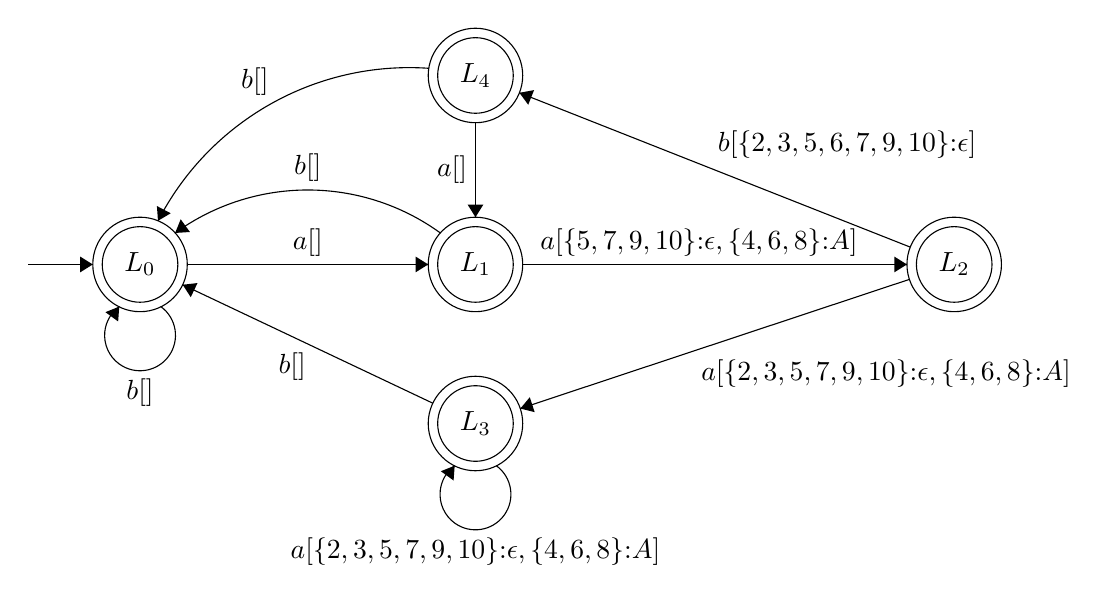
\begin{tikzpicture}[scale=0.2]
					\tikzstyle{every node}+=[inner sep=0pt]
					\draw [black] (14.7,-29.5) circle (3);
					\draw (14.7,-29.5) node {$L_0$};
					\draw [black] (14.7,-29.5) circle (2.4);
					\draw [black] (36,-29.5) circle (3);
					\draw (36,-29.5) node {$L_1$};
					\draw [black] (36,-29.5) circle (2.4);
					\draw [black] (66.4,-29.5) circle (3);
					\draw (66.4,-29.5) node {$L_2$};
					\draw [black] (66.4,-29.5) circle (2.4);
					\draw [black] (36,-39.6) circle (3);
					\draw (36,-39.6) node {$L_3$};
					\draw [black] (36,-39.6) circle (2.4);
					\draw [black] (36,-17.5) circle (3);
					\draw (36,-17.5) node {$L_4$};
					\draw [black] (36,-17.5) circle (2.4);
					\draw [black] (17.7,-29.5) -- (33,-29.5);
					\fill [black] (33,-29.5) -- (32.2,-29) -- (32.2,-30);
					\draw (25.35,-29) node [above] {$a[]$};
					\draw [black] (16.023,-32.18) arc (54:-234:2.25);
					\draw (14.7,-36.75) node [below] {$b[]$};
					\fill [black] (13.38,-32.18) -- (12.5,-32.53) -- (13.31,-33.12);
					\draw [black] (7.6,-29.5) -- (11.7,-29.5);
					\fill [black] (11.7,-29.5) -- (10.9,-29) -- (10.9,-30);
					\draw [black] (39,-29.5) -- (63.4,-29.5);
					\fill [black] (63.4,-29.5) -- (62.6,-29) -- (62.6,-30);
					\draw (50.2,-29) node [above] {$a[\{5,7,9,10\}{:}\epsilon,\{4,6,8\}{:}A]$};
					\draw [black] (16.929,-27.5) arc (125.91094:54.08906:14.357);
					\fill [black] (16.93,-27.5) -- (17.87,-27.44) -- (17.28,-26.63);
					\draw (25.35,-24.27) node [above] {$b[]$};
					\draw [black] (63.55,-30.45) -- (38.85,-38.65);
					\fill [black] (38.85,-38.65) -- (39.76,-38.88) -- (39.45,-37.93);
					\draw (62.07,-35.5) node [below] {$a[\{2,3,5,7,9,10\}{:}\epsilon,\{4,6,8\}{:}A]$};
					\draw [black] (63.61,-28.4) -- (38.79,-18.6);
					\fill [black] (38.79,-18.6) -- (39.35,-19.36) -- (39.72,-18.43);
					\draw (59.6,-22.83) node [above] {$b[\{2,3,5,6,7,9,10\}{:}\epsilon]$};
					\draw [black] (37.323,-42.28) arc (54:-234:2.25);
					\draw (36,-46.85) node [below] {$a[\{2,3,5,7,9,10\}{:}\epsilon,\{4,6,8\}{:}A]$};
					\fill [black] (34.68,-42.28) -- (33.8,-42.63) -- (34.61,-43.22);
					\draw [black] (33.29,-38.31) -- (17.41,-30.79);
					\fill [black] (17.41,-30.79) -- (17.92,-31.58) -- (18.35,-30.68);
					\draw (24.36,-35.06) node [below] {$b[]$};
					\draw [black] (15.844,-26.731) arc (152.76293:86.02918:17.941);
					\fill [black] (15.84,-26.73) -- (16.65,-26.25) -- (15.77,-25.79);
					\draw (21.99,-18.81) node [above] {$b[]$};
					\draw [black] (36,-20.5) -- (36,-26.5);
					\fill [black] (36,-26.5) -- (36.5,-25.7) -- (35.5,-25.7);
					\draw (35.5,-23.5) node [left] {$a[]$};
				\end{tikzpicture}
			\end{center}
			\caption{The left automaton of the bimachine with final output from example~\ref{ex:bmfo}. The output function $\psi$ is also shown. A transition from $L_i$ into $L_j$ of the form $x[\mathrm{SET}_0{:}y_0, \ldots, \mathrm{SET}_p{:}y_p]$ denotes that
			\[ \delta_L(L_i, x)=L_j \text{ and } (\forall p'\le p)(\forall k\in \mathrm{SET}_{p'})\psi(L_i, x, R_k)=y_{p'}. \]
			Unless otherwise specified, $\psi(L, x, R)=x$.}
			\label{fig:ex:bmfo:A_L}
		\end{figure}
		
		The execution of $\mathcal{B}$ over $t=aaaaaabaaab$ is shown on figure~\ref{fig:ex:bmfo:execution}.
		\begin{figure}[h]
			\begin{adjustbox}{center=\textwidth}
				\setlength\tabcolsep{3pt} % default value: 6pt
				\begin{tabular}{*{23}{c}}
					${R_{10}}$ &$\xleftarrow{a}$& ${R_{10}}$ &$\xleftarrow{a}$& ${R_{10}}$ &$\xleftarrow{a}$& ${R_{10}}$ &$\xleftarrow{a}$& ${R_7}$ &$\xleftarrow{a}$& ${R_8}$
					&$\xleftarrow{a}$& ${R_5}$ &$\xleftarrow{b}$& ${R_{10}}$ &$\xleftarrow{a}$& ${R_7}$ &$\xleftarrow{a}$& $R_4$ &$\xleftarrow{a}$& ${R_2}$
					&$\xleftarrow{b}$& $R_0$ \\
					$L_0$ &$\xrightarrow{a}$& ${L_1}$ &$\xrightarrow{a}$& ${L_2}$ &$\xrightarrow{a}$& ${L_3}$ &$\xrightarrow{a}$& ${L_3}$ &$\xrightarrow{a}$& ${L_3}$
					&$\xrightarrow{a}$& ${L_3}$ &$\xrightarrow{b}$& $L_0$ &$\xrightarrow{a}$& ${L_1}$ &$\xrightarrow{a}$& ${L_2}$ &$\xrightarrow{a}$& ${L_3}$
					&$\xrightarrow{b}$& $L_0$ \\
					%0 && 1 && 2 && 3 && 4 && 5 && 6 && 7 && 8 && 9 && 10 && 11 \\
					& $a$ && $\epsilon$ && $\epsilon$ && $\epsilon$ && $A$ && $\epsilon$ && $b$ && $a$ && $A$ && $\epsilon$ && $b$ & \\
				\end{tabular}
			\end{adjustbox}
			\caption{The execution of $\mathcal{B}$ over $t=aaaaaabaaab$. \\
				$\mathrm{Out}_\mathcal{B}(t) = a\epsilon\epsilon\epsilon A\epsilon baA\epsilon b\cdot\iota(L_0) = aAbaAb$.}
			\label{fig:ex:bmfo:execution}
		\end{figure}
	\end{example}
	
	\begin{proposition} \label{prop:construction_classical_bimachine_correctness}
		Construction~\ref{constr:classical_bimachine} correctly defines a classical bimachine with final output.
	\end{proposition}
	\begin{proof}
		For the correctness of $A_R$, see proposition~\ref{prop:construction_two-step_bimachine_correctness}.
		Clearly, $\phi_0$ and $\iota$ are correctly defined.
		
		Let $(L, \phi)\in Q_L$, $a\in \Sigma_1$, $(R', g')\in Q_R$ and $(R, g) = \delta_R((R', g'), a)$. We will show that
		\[ (L', \phi') = \delta_L((L, \phi), a) \]
		is correctly defined.
		
		If $\mathrm{NonemptyMatchNotFinished}(\phi, (R, g))$, then $\phi((R,g))\in \Rng(g)\setminus F_T$.
		We can conclude that $\mu(\phi((R,g)), a, g')$ is defined in exactly the same way as in the proof of the correctness for $\delta$ in proposition~\ref{prop:construction_two-step_bimachine_correctness}.
		Again, all elements of $\{ i' \mid (\phi((R,g)), a, g'(i'))\in \Delta_T^{\Sigma_1} \}$ belong to the domain of $g'$ and in particular $\mu(\phi((R,g)), a, g')$ does. Thus $g'(\mu(\phi((R,g)), a, g'))$ is defined.
		
		If $\mathrm{NonemptyMatchBegin}(L, g)$, then $I(L, g)\ne\emptyset$. Let $q = \nu(L, g)$. By the definitions of $I$ and $\nu$, we have $q\in S_T$ and $q\in \Rng(g)$ which implies $q\in \Rng(g)\setminus F_T$. To see that $g'(\mu(\nu(L, g), a, g'))$ is defined, the same reasoning as in the previous case can be used.
		
		Finally, if $\mathrm{NonemptyMatchBegin}(L', g')$, immediately follows that $\nu(L', g')$ is defined. Thus $\phi'$ is correctly defined.
		
		For $\psi$, if $\mathrm{NonemptyMatchNotFinished}(\phi, (R, g))$, then $(\phi((R,g)), a, \phi((R',g')))\in \Delta_T^{\Sigma_1}$, so
		\[ \{ m\mid (\phi((R,g)), (a, m), \phi((R',g')))\in \Delta_T \}\ne\emptyset \]
		and hence $\mathrm{Output}(\phi((R,g)), a, \phi'((R',g')))$ is defined.
		
		Similarly, if $\mathrm{NonemptyMatchFinished}(\phi, (R, g)) \mathbin\& \mathrm{NonemptyMatchBegin}(L, g)$, then 
		\[ \{ m\mid (\nu(L, g), (a, m), \phi((R',g')))\in \Delta_T \}\ne\emptyset \]
		and $\mathrm{Output}(\nu(L, g), a, \phi'((R',g')))$ is defined.
		If $\mathrm{EmptyMatchBegin}(L, R)$, it follows directly from the definitions that $\mathcal{E}_{\min(J(L, R))}$ is defined.
		Thus $\psi$ is correctly defined.
	\end{proof}

	Let $A = (\Sigma_1, \Sigma_2, A_L, A_R, Q, q_\mathrm{err}, \delta, \tau, \psi_\delta, \psi_\tau)$ be obtained from construction~\ref{constr:two-step_bimachine}
	and $\mathcal{B} = (\Sigma_1\cup\Sigma_2, A_L', A_R, \psi, \iota)$ be obtained from construction~\ref{constr:classical_bimachine} applied on the same FSR $((\mathcal{T}_r, \mathcal{E}_r, A_{\lambda_r}, A_{\rho_r}))_{r=1}^m$.
	We are going to show that $A$ and $\mathcal{B}$ are equivalent, i.e.\ for each input string $t\in \Sigma_1^*$, both $A$ and $\mathcal{B}$ produce the same output for $t$.
	For this purpose, we are going to prove a couple of propositions which show the relationships between the two machines.
	
	Let $t=t_1\ldots t_n\in \Sigma_1^*$,
	\[ ((L_i, q_i, \overline{q_i}, (R_i, g_i), o_i, \overline{o_i}))_{i=0}^n \]
	be an execution of $A$ over $t$ and 
	\[ (((L_i, \phi_i), o_i', (R_i, g_i)))_{i=0}^n \]
	be an execution of $\mathcal{B}$ over $t$.
	Note that the executions of the right automata of the two bimachines coincide since they both have the same automaton $A_R$ as right automaton. Similarly, the $L_i$ components in both executions coincide since they are constructed in one and the same way.
	
	The first proposition will show the relationship between the states of $A$ and the "selected" states by the functions $\phi_i$.
	\begin{proposition} \label{prop:relationship_between_states_of_two-step_and_classical_bimachine}
		Let $0\le i\le n$. All of the following implications hold:
		\begin{eqnarray}
			q_i\in Q_T\setminus S_T &\implies& \phi_i((R_i, g_i)) = q_i,
				\label{prop:relationship_between_states_of_two-step_and_classical_bimachine:eq1} \\
			q_i = q_\mathrm{err} \mathbin\& \overline{q_i} = q_\mathrm{err} &\implies& \phi_i((R_i, g_i))\uparrow,
				\label{prop:relationship_between_states_of_two-step_and_classical_bimachine:eq2} \\
			q_i\notin F_T \mathbin\& \overline{q_i}\in S_T &\implies& \phi_i((R_i, g_i)) = \overline{q_i}.
				\label{prop:relationship_between_states_of_two-step_and_classical_bimachine:eq4}
		\end{eqnarray}
	\end{proposition}
	\begin{proof}
		Assume that the implications hold for all $j<i$.
		\begin{description}
			\item[(\ref{prop:relationship_between_states_of_two-step_and_classical_bimachine:eq1})]
				Assume $q_i\in Q_T\setminus S_T$. Then $i>0$ ($q_0 = q_\mathrm{err}\notin Q_T$) and
				$\overline{q_{i-1}}\in \Rng(g_{i-1})\setminus F_T$.
				\begin{description}
				\item[Case 1:] $\overline{q_{i-1}}\notin S_T$.
					Then $\overline{q_{i-1}} = q_{i-1}$ and hence $q_{i-1}\in Q_T\setminus S_T$.
					By the i.h. for~(\ref{prop:relationship_between_states_of_two-step_and_classical_bimachine:eq1}),
					$\phi_{i-1}((R_{i-1}, g_{i-1})) = q_{i-1}$.
					Therefore $\phi_{i-1}((R_{i-1}, g_{i-1}))\downarrow$ and $\phi_{i-1}((R_{i-1}, g_{i-1}))\in \Rng(g_{i-1})\setminus F_T$, i.e.
					\[ \mathrm{NonemptyMatchNotFinished}(\phi_{i-1}, (R_{i-1}, g_{i-1})). \]
					We conclude that
					\begin{eqnarray*}
						\phi_i((R_i, g_i)) &=& g_i(\mu(\phi_{i-1}((R_{i-1}, g_{i-1})), t_i, g_i)) \\
							&=& g_i(\mu(\overline{q_{i-1}}, t_i, g_i)) = q_i.
					\end{eqnarray*}
				\item[Case 2:] $\overline{q_{i-1}}\in S_T$.
					Then $q_{i-1}\notin Q_T\setminus F_T$, $I(L_{i-1}, g_{i-1})\ne\emptyset$ and $\overline{q_{i-1}} = \nu(L_{i-1}, g_{i-1})$. Therefore in this case we have $\mathrm{NonemptyMatchBegin}(L_{i-1}, g_{i-1})$.
					\begin{description}
					\item[Case 2.1:] $q_{i-1}\in F_T$.
						But since $F_T\subseteq Q_T\setminus S_T$, by i.h. for~(\ref{prop:relationship_between_states_of_two-step_and_classical_bimachine:eq1}) we have $\phi_{i-1}((R_{i-1}, g_{i-1})) = q_{i-1}$.
						Thus $\mathrm{NonemptyMatchFinished}(\phi_{i-1}, (R_{i-1}, g_{i-1}))$ holds.
						We conclude that
						\begin{eqnarray*}
							\phi_i((R_i, g_i)) &=& g_i(\mu(\nu(L_{i-1}, g_{i-1}), t_i, g_i)) \\
							&=& g_i(\mu(\overline{q_{i-1}}, t_i, g_i)) = q_i.
						\end{eqnarray*}
					\item[Case 2.2:] $q_{i-1}\notin F_T$. Then $q_{i-1} = q_\mathrm{err}$.
						By i.h. for~(\ref{prop:relationship_between_states_of_two-step_and_classical_bimachine:eq4}),
						$\phi_{i-1}((R_{i-1}, g_{i-1})) = \overline{q_{i-1}}$.
						We have $\overline{q_{i-1}}\in S_T\subseteq Q_T$, so by proposition~\ref{prop:execution_is_correct} we get $\overline{q_{i-1}}\in \Rng(g_{i-1})\setminus F_T$.
						Therefore, as in case 1, we have $\mathrm{NonemptyMatchNotFinished}(\phi_{i-1}, (R_{i-1}, g_{i-1}))$ and
						$\phi_i((R_i, g_i)) = q_i$.
					\end{description}
				\end{description}
			\item[(\ref{prop:relationship_between_states_of_two-step_and_classical_bimachine:eq2})]
				Assume $q_i = \overline{q_i} = q_\mathrm{err}$. Then $I(L_i, g_i) = \emptyset$, i.e.\ $\lnot\mathrm{NonemptyMatchBegin}(L_i, g_i)$.
				\begin{description}
				\item[Case 1:] $i=0$.
					Then $L_i = L_0 = S_\lambda$, so $\lnot\mathrm{NonemptyMatchBegin}(S_\lambda, g_i)$ and hence $\phi_i((R_i, g_i))\uparrow$.
				\item[Case 2:] $i>0$.
					Then $q_i = q_\mathrm{err}$ implies $\overline{q_{i-1}} = \tau(q_{i-1}, L_{i-1}, (R_{i-1}, g_{i-1})) = q_\mathrm{err}$. Therefore $q_{i-1}\notin Q_T\setminus F_T$ and $I(L_{i-1}, g_{i-1}) = \emptyset$, i.e.
					\[ \lnot\mathrm{NonemptyMatchBegin}(L_{i-1}, g_{i-1}). \]
					\begin{description}
					\item[Case 2.1:] $q_{i-1}\in F_T$.
						Then, since $F_T\subseteq Q_T\setminus S_T$, by the i.h. for~(\ref{prop:relationship_between_states_of_two-step_and_classical_bimachine:eq1}), $\phi_{i-1}((R_{i-1}, g_{i-1})) = q_{i-1}\notin \Rng(g_{i-1})\setminus F_T$. Therefore
						\[ \lnot\mathrm{NonemptyMatchNotFinished}(\phi_{i-1}, (R_{i-1}, g_{i-1})). \]
					\item[Case 2.2:] $q_{i-1}\notin F_T$. Then $q_{i-1} = q_\mathrm{err}$.
						By the i.h. for~(\ref{prop:relationship_between_states_of_two-step_and_classical_bimachine:eq2}), $\phi_{i-1}((R_{i-1}, g_{i-1}))\uparrow$. Therefore again
						\[ \lnot\mathrm{NonemptyMatchNotFinished}(\phi_{i-1}, (R_{i-1}, g_{i-1})). \]
					\end{description}
					We have shown that none of the three conditions for $\phi_i((R_i, g_i))$ to be defined is satisfied, so $\phi_i((R_i, g_i))\uparrow$.
				\end{description}
			\item[(\ref{prop:relationship_between_states_of_two-step_and_classical_bimachine:eq4})]
				Assume $q_i\notin F_T$ and $\overline{q_i}\in S_T$. Then $q_i\notin Q_T\setminus F_T$, $I(L_i, g_i)\ne \emptyset$ and $\overline{q_i} = \nu(L_i, g_i)$. Therefore in this case we have $\mathrm{NonemptyMatchBegin}(L_i, g_i)$. Since $q_i\notin F_T$, we have $q_i = q_\mathrm{err}$.
				\begin{description}
				\item[Case 1:] $i=0$.
					Then $L_i = L_0 = S_\lambda$, so $\mathrm{NonemptyMatchBegin}(S_\lambda, g_i)$ and hence
					\[ \phi_i((R_i, g_i)) = \nu(S_\lambda, g_i) = \nu(L_i, g_i) = \overline{q_i}. \]
				\item[Case 2:] $i>0$.
					In this case $\overline{q_{i-1}} = q_\mathrm{err}$. Therefore $q_{i-1}\notin Q_T\setminus F_T$ and $I(L_{i-1}, g_{i-1}) = \emptyset$, i.e.\ $\lnot\mathrm{NonemptyMatchBegin}(L_{i-1}, g_{i-1})$.
					\begin{description}
					\item[Case 2.1:] $q_{i-1}\in F_T$.
						Then, since $F_T\subseteq Q_T\setminus S_T$, by the i.h. for~(\ref{prop:relationship_between_states_of_two-step_and_classical_bimachine:eq1}) we get $\phi_{i-1}((R_{i-1}, g_{i-1})) = q_{i-1}$.
						Thus we have
						\[ \mathrm{NonemptyMatchFinished}(\phi_{i-1}, (R_{i-1}, g_{i-1})). \]
					\item[Case 2.2:] $q_{i-1}\notin F_T$. Then $q_{i-1} = q_\mathrm{err}$. By the i.h. for~(\ref{prop:relationship_between_states_of_two-step_and_classical_bimachine:eq2}), $\phi_{i-1}((R_{i-1}, g_{i-1}))\uparrow$. Thus we have
					\[ \mathrm{OutsideOfMatch}(\phi_{i-1}, (R_{i-1}, g_{i-1})). \]
					\end{description}
					In either case $\phi_i((R_i, g_i)) = \nu(L_i, g_i) = \overline{q_i}$.
				\end{description}
		\end{description}
	\end{proof}
	The next two proposition show the relationship between the outputs of the two bimachines at any particular step.
	\begin{proposition} \label{prop:relationship_between_outputs_of_two-step_and_classical_bimachine}
		Let $0\le i < n$. Then \( \overline{o_i}\cdot o_{i+1} = o_i' \).
	\end{proposition}
	\begin{proof}
		In the following proof we will tacitly use the result of proposition~\ref{prop:execution_outputs_are_unique}.
		\begin{description}
		\item[Case 1:] $q_{i+1}\in Q_T$.
			Then $\overline{q_i}\in \Rng(g_i)\setminus F_T$ and $o_{i+1} = \mathrm{Output}(\overline{q_i}, t_{i+1}, q_{i+1})$.
			Note that $q_{i+1}\notin S_T$, so we can apply~(\ref{prop:relationship_between_states_of_two-step_and_classical_bimachine:eq1}) to get $\phi_{i+1}((R_{i+1}, g_{i+1})) = q_{i+1}$.
			We have $\tau(q_i, L_i, (R_i, g_i)) = \overline{q_i}\ne q_\mathrm{err}$, so $\overline{o_i} = \epsilon$.
			\begin{description}
			\item[Case 1.1:] $\overline{q_i}\notin S_T$. Then $\overline{q_i} = q_i\in Q_T\setminus S_T$.
				By~(\ref{prop:relationship_between_states_of_two-step_and_classical_bimachine:eq1}), $\phi_i((R_i, g_i)) = q_i$.
				Note that $\overline{q_i}\notin F_T$ and $\overline{q_i} = q_i$, so $\phi_i((R_i, g_i))\in Q_T\setminus F_T$, that is
				\[ \mathrm{NonemptyMatchNotFinished}(\phi_i, (R_i, g_i)). \]
				Thus
				\begin{eqnarray*}
					o_i' &=& \psi(L_i, t_{i+1}, (R_{i+1}, g_{i+1})) \\
						&=& \mathrm{Output}(\phi_i((R_i, g_i)), t_{i+1}, \phi_{i+1}((R_{i+1}, g_{i+1}))) \\
						&=& \mathrm{Output}(q_i, t_{i+1}, q_{i+1}) \\
						&=& \mathrm{Output}(\overline{q_i}, t_{i+1}, q_{i+1}) = o_{i+1} = \overline{o_i}\cdot o_{i+1}.
				\end{eqnarray*}
			\item[Case 1.2:] $\overline{q_i}\in S_T$.
				Then $q_i\notin Q_T\setminus F_T$, $I(L_i, g_i)\ne \emptyset$ and $\overline{q_i} = \nu(L_i, g_i)$. Therefore in this case we have $\mathrm{NonemptyMatchBegin}(L_i, g_i)$.
				\begin{description}
				\item[Case 1.2.1:] $q_i\in F_T$.
					Then $q_i\in Q_T\setminus S_T$ and by~(\ref{prop:relationship_between_states_of_two-step_and_classical_bimachine:eq1}) we have $\phi_i((R_i, g_i)) = q_i\in F_T$. This means
					\[ \mathrm{NonemptyMatchFinished}(\phi_i, (R_i, g_i)) \]
					and thus
					\begin{eqnarray*}
						o_i' &=& \mathrm{Output}(\nu(L_i, g_i), t_{i+1}, \phi_{i+1}((R_{i+1}, g_{i+1}))) \\
							&=& \mathrm{Output}(\overline{q_i}, t_{i+1}, q_{i+1}) = o_{i+1} = \overline{o_i}\cdot o_{i+1}.
					\end{eqnarray*}
				\item[Case 1.2.2:] $q_i\notin F_T$.
					Then, by~(\ref{prop:relationship_between_states_of_two-step_and_classical_bimachine:eq4}), $\phi_i((R_i, g_i)) = \overline{q_i}\in S_T\subseteq Q_T$.
					By proposition~\ref{prop:execution_is_correct}, $\overline{q_i}\in \Rng(g_i)\setminus F_T$, so $\phi_i((R_i, g_i))\in \Rng(g_i)\setminus F_T$. Therefore, we have
					\[ \mathrm{NonemptyMatchNotFinished}(\phi_i, (R_i, g_i)) \]
					and thus
					\begin{eqnarray*}
						o_i' &=& \psi(L_i, t_{i+1}, (R_{i+1}, g_{i+1})) \\
							&=& \mathrm{Output}(\phi_i((R_i, g_i)), t_{i+1}, \phi_{i+1}((R_{i+1}, g_{i+1}))) \\
							&=& \mathrm{Output}(\overline{q_i}, t_{i+1}, q_{i+1}) = o_{i+1} = \overline{o_i}\cdot o_{i+1}.
					\end{eqnarray*}
				\end{description}
			\end{description}
		\item[Case 2:] $q_{i+1}\notin Q_T$. Then $q_{i+1} = q_\mathrm{err}$ and $o_{i+1} = t_{i+1}$.
			We also have that $\overline{q_i} = q_\mathrm{err}$, so $q_i\notin Q_T\setminus F_T$ and $I(L_i, g_i) = \emptyset$, i.e.
			\[ \lnot\mathrm{NonemptyMatchBegin}(L_i, g_i). \]
			If $q_i\in F_T$, then (by~(\ref{prop:relationship_between_states_of_two-step_and_classical_bimachine:eq1})) $q_i = \phi_i((R_i, g_i))\in F_T$, that is
			\[ \mathrm{NonemptyMatchFinished}(\phi_i, (R_i, g_i)) \]
			and 
			\[ \lnot\mathrm{NonemptyMatchNotFinished}(\phi_i, (R_i, g_i)). \]
			Otherwise $q_i = q_\mathrm{err}$ and (by~(\ref{prop:relationship_between_states_of_two-step_and_classical_bimachine:eq2})) $\phi_i((R_i, g_i))\uparrow$.
			In either case we have
			\[ \lnot\mathrm{NonemptyMatchNotFinished}(\phi_i, (R_i, g_i)) \]
			and
			\[ \mathrm{OutsideOfMatch}(\phi_i, (R_i, g_i))\mathbin\lor\mathrm{NonemptyMatchFinished}(\phi_i, (R_i, g_i)). \]
			\begin{description}
			\item[Case 2.1:] $J(L_i, R_i)\ne\emptyset$ ($\mathrm{EmptyMatchBegin}(L_i, R_i)$).
				Then, since $\overline{q_i} = q_\mathrm{err}$, we have $\overline{o_i} = \mathcal{E}_{\min(J(L_i, R_i))}$.
				In this case
				\[ o_i' = \mathcal{E}_{\min(J(L_i, R_i))}\cdot t_{i+1} = \overline{o_i}\cdot o_{i+1}. \]
			\item[Case 2.2:] $J(L_i, R_i) = \emptyset$ ($\lnot\mathrm{EmptyMatchBegin}(L_i, R_i)$).
				Then $\overline{o_i} = \epsilon$. In this case
				\[ o_i' = t_{i+1} = o_{i+1} = \overline{o_i}\cdot o_{i+1}. \]
			\end{description}
		\end{description}
	\end{proof}

	\begin{proposition} \label{prop:relationship_between_outputs_last_step_of_two-step_and_classical_bimachine}
		\( \overline{o_n} = o_n' \).
	\end{proposition}
	\begin{proof}
		By proposition~\ref{prop:execution_last_state}, $\tau(q_n, L_n, (R_n, g_n)) = \overline{q_n} = q_\mathrm{err}$.
		By definition, $(R_n, g_n) = s_R = (S_{RU}, g_s)$.
		Therefore, if $J(L_n, R_n)\ne \emptyset$, then
		\[ \overline{o_n} = \mathcal{E}_{\min(J(L_n, R_n))} = \mathcal{E}_{\min(J(L_n, S_{RU}))} = o_n'. \]
		Otherwise \( \overline{o_n} = o_n' = \epsilon \).
	\end{proof}
	We are now ready to show that $A$ and $\mathcal{B}$ are equivalent.
	\begin{theorem} \label{thm:two_step_bimachines_and_classical_bimachines_equvalence}
		\( \mathrm{Out}_A(t) = \mathrm{Out}_\mathcal{B}(t) \).
	\end{theorem}
	\begin{proof}
		Applying proposition~\ref{prop:relationship_between_outputs_of_two-step_and_classical_bimachine} $n$ times gives
		\[ \overline{o_0}o_1\overline{o_1}o_2\ldots \overline{o_{n-1}}o_n = o_0'o_1'\ldots o_{n-1}'. \]
		Finally, we use proposition~\ref{prop:relationship_between_outputs_last_step_of_two-step_and_classical_bimachine} and the fact that $o_0 = \epsilon$ by definition to get
		\[ \mathrm{Out}_A(t) = o_0\overline{o_0}o_1\overline{o_1}o_2\ldots \overline{o_{n-1}}o_n\overline{o_n} = o_0'o_1'\ldots o_{n-1}'o_n' = \mathrm{Out}_\mathcal{B}(t) \]
		which completes the proof.
	\end{proof}

	\section{Complexity analysis} \label{section:complexity}
	\begin{proposition} \label{prop:enum_subsets_count}
		Let Q be a finite set with $\len{Q}\ge 2$. The number of the enumerations of subsets of Q is less than $3\len{Q}!$.
	\end{proposition}
	\begin{proof}
		Let $n = \len{Q}$.
		The number of the subsets of Q can be expressed as
		\[ \sum_{k=0}^{n} \binom{n}{k}. \]
		A subset of $k$ element has $k!$ distinct enumerations (the permutations of the elements), so the total number of enumerations is
		\[ \sum_{k=0}^{n} k!\binom{n}{k}. \]
		Using our assumption that $\len{Q}\ge 2$ and the fact that $(n-k)!\ge 2^{n-k}$ for $k\le n-2$ we obtain an upper bound for this total number of enumerations:
		\begin{eqnarray*}
			\sum_{k=0}^{n} k!\binom{n}{k} &=& \sum_{k=0}^{n} \frac{n!}{(n-k)!} = 2n! + \sum_{k=0}^{n-2} \frac{n!}{(n-k)!} \\
				&\le& 2n! + \sum_{k=0}^{n-2} \frac{n!}{2^{n-k}} = 2n! + n!\sum_{p=2}^{n} \frac{1}{2^p} < 3n!\in O(n!).
		\end{eqnarray*}
	\end{proof}

	\begin{proposition} \label{prop:size_two-step_bimachine}
		Let $A = (\Sigma_1, \Sigma_2, A_L, A_R, Q, q_\mathrm{err}, \delta, \tau, \psi_\delta, \psi_\tau)$ be obtained from construction~\ref{constr:two-step_bimachine} applied on some FSR $((\mathcal{T}_r, \mathcal{E}_r, A_{\lambda_r}, A_{\rho_r}))_{r=1}^m$. Let $Q_\rho = \bigcup_{r=1}^m Q_{\rho_r}$. Then
		\begin{eqnarray*}
			\len{Q_L} &\le& 2^{\len{Q_\lambda}}, \\
			\len{\delta_L} &=& \len{Q_L}\cdot \len{\Sigma_1} \le 2^{\len{Q_\lambda}}\cdot \len{\Sigma_1}, \\
			\len{Q_R} &\le& 2^{\len{Q_\rho}}\cdot 3\len{Q_T}!\in O(2^{\len{Q_\rho}}\cdot \len{Q_T}!), \\
			\len{\delta_R} &=& \len{Q_R}\cdot \len{\Sigma_1} \le 2^{\len{Q_\rho}}\cdot 3\len{Q_T}!\cdot \len{\Sigma_1}, \\
			\len{\delta} = \len{\psi_\delta} &\le& \len{\Sigma_1}\cdot 2^{\len{Q_\rho}}\cdot 3(\len{Q_T}+1)!
				\in O(\len{\Sigma_1}\cdot 2^{\len{Q_\rho}}\cdot(\len{Q_T}+1)!), \\
			\len{\tau} = \len{\psi_\tau} &\le& 2^{\len{Q_\lambda}}\cdot 2^{\len{Q_\rho}}\cdot 3(\len{Q_T}+1)!
				\in O(2^{\len{Q_\lambda}+\len{Q_\rho}}\cdot(\len{Q_T}+1)!), \\
			\Rng(\delta) &\le& \len{Q_T} + 1, \\
			\Rng(\tau) &\le& \len{Q_T} + 1.
		\end{eqnarray*}
		The total size of $A$ is
		\begin{eqnarray*}
			&&\len{\delta_L} + \len{\delta_R} + \len{\delta} + \len{\psi_\delta} + \len{\tau} + \len{\psi_\tau} \\
			&\le& (2^{\len{Q_\lambda}} + 2^{\len{Q_\rho}}\cdot 3\len{Q_T}!)\cdot\len{\Sigma_1} + 6\cdot 2^{\len{Q_\rho}}\cdot (\len{Q_T}+1)!\cdot(2^{\len{Q_\lambda}} + \len{\Sigma_1}) \\
			&\in& O(2^{\len{Q_\rho}}\cdot(\len{Q_T}+1)!\cdot (2^{\len{Q_\lambda}} + \len{\Sigma_1}) + 2^{\len{Q_\lambda}}\cdot \len{\Sigma_1}).
		\end{eqnarray*}
	\end{proposition}
	\begin{proof}
		The number of states of $A_\lambda$ is
		\[ \len{Q_\lambda} = \sum_{r=1}^{m} \len{Q_{\lambda_r}}. \]
		The number of states of $A_L$ is at most $2^{\len{Q_\lambda}}$.

		Assuming $\len{Q_T}\ge 2$ (which is always the case unless the batch of rules is empty),
		an obvious upper bound for the number of states of $A_R$ is
		\[ \len{Q_R} \le 2^{\len{Q_{RU}}} \sum_{k=0}^{\len{Q_T}} k!\binom{\len{Q_T}}{k}
			\le 2^{\len{Q_{RU}}}\cdot 3\len{Q_T}!\in O(2^{\len{Q_{RU}}}\cdot \len{Q_T}!).
		\]

		If we look more carefully, we can see that for each $g\in\bigcup_{Q\subseteq Q_T} \mathrm{Enum}(Q)$, the number of pairs $(R, g)$ which may belong to $Q_R$ is no greater than $2^{\len{Q_\rho}}$. This is because, for any $(R, g)\in Q_R$, the states of $Q_T$ which belong to R are exactly the states in $\Rng(g)$. This observation gives us a more precise upper bound for the states of $Q_R$:
		\[ \len{Q_R} \le 2^{\len{Q_\rho}} \sum_{k=0}^{\len{Q_T}} k!\binom{\len{Q_T}}{k}
			\le 2^{\len{Q_\rho}}\cdot 3\len{Q_T}!\in O(2^{\len{Q_\rho}}\cdot \len{Q_T}!).
		\]
		
		For the transition functions and the output functions of $A$ we have the following upper bounds:
		\begin{eqnarray*}
			\len{\delta} = \len{\psi_\delta} &=& (\len{Q_T}+1)\cdot\len{\Sigma_1}\cdot\len{Q_R} \\
				&\le& (\len{Q_T}+1)\cdot\len{\Sigma_1}\cdot 2^{\len{Q_\rho}}\cdot 3\len{Q_T}!
				\in O(\len{\Sigma_1}\cdot 2^{\len{Q_\rho}}\cdot(\len{Q_T}+1)!), \\
			\len{\tau} = \len{\psi_\tau} &=& (\len{Q_T}+1)\cdot\len{Q_L}\cdot\len{Q_R} \\
				&\le& (\len{Q_T}+1)\cdot2^{\len{Q_\lambda}}\cdot 2^{\len{Q_\rho}}\cdot 3\len{Q_T}!
				\in O(2^{\len{Q_\lambda}+\len{Q_\rho}}\cdot(\len{Q_T}+1)!).
		\end{eqnarray*}
	\end{proof}

	\begin{proposition} \label{prop:size_classical_bimachine}
		Let $\mathcal{B} = (\Sigma_1\cup\Sigma_2, A_L, A_R, \psi, \iota)$ be obtained from construction~\ref{constr:classical_bimachine} applied on some FSR $((\mathcal{T}_r, \mathcal{E}_r, A_{\lambda_r}, A_{\rho_r}))_{r=1}^m$. Let $Q_\rho = \bigcup_{r=1}^m Q_{\rho_r}$. Then
		\begin{eqnarray*}
			\len{Q_R} &\le& 2^{\len{Q_\rho}}\cdot 3\len{Q_T}!\in O(2^{\len{Q_\rho}}\cdot \len{Q_T}!), \\
			\len{\delta_R} &=& \len{Q_R}\cdot \len{\Sigma_1} \le 2^{\len{Q_\rho}}\cdot 3\len{Q_T}!\cdot \len{\Sigma_1}, \\
			\len{\iota} = \len{Q_L} &\le& 2^{\len{Q_\lambda}}\cdot (\len{Q_T}+1)^{3\len{Q_T}!} \in O(2^{\len{Q_\lambda}}\cdot \len{Q_T}^{3\len{Q_T}!}), \\
			\len{\delta_L} &=& \len{Q_L}\cdot \len{\Sigma_1} \le 2^{\len{Q_\lambda}}\cdot (\len{Q_T}+1)^{3\len{Q_T}!}\cdot \len{\Sigma_1}, \\
			\len{\psi} &\le& 2^{\len{Q_\lambda}+\len{Q_\rho}}\cdot (\len{Q_T}+1)^{3\len{Q_T}!}\cdot \len{\Sigma_1}\cdot 3\len{Q_T}! \\
			&\in& O(2^{\len{Q_\lambda}+\len{Q_\rho}}\cdot \len{Q_T}^{3\len{Q_T}!}\cdot \len{\Sigma_1}\cdot \len{Q_T}!).
		\end{eqnarray*}
		The total size of $\mathcal{B}$ is
		\begin{eqnarray*}
			&&\len{\delta_R} + \len{\delta_L} + \len{\iota} + \len{\psi} \\
			&\le& 2^{\len{Q_\rho}}\cdot 3\len{Q_T}!\cdot \len{\Sigma_1} + 2^{\len{Q_\lambda}}\cdot (\len{Q_T}+1)^{3\len{Q_T}!}\cdot(\len{\Sigma_1}+1)
				+ 2^{\len{Q_\lambda}+\len{Q_\rho}}\cdot (\len{Q_T}+1)^{3\len{Q_T}!}\cdot \len{\Sigma_1}\cdot 3\len{Q_T}! \\
			&=& 2^{\len{Q_\rho}}\cdot 3\len{Q_T}!\cdot \len{\Sigma_1} + 2^{\len{Q_\lambda}}\cdot (\len{Q_T}+1)^{3\len{Q_T}!}\cdot (\len{\Sigma_1}+1+2^{\len{Q_\rho}}\cdot \len{\Sigma_1}\cdot 3\len{Q_T}!) \\
			&\in& O(2^{\len{Q_\lambda}+\len{Q_\rho}}\cdot \len{Q_T}^{3\len{Q_T}!}\cdot \len{\Sigma_1}\cdot \len{Q_T}!).
		\end{eqnarray*}
	\end{proposition}
	\begin{proof}
		The number of states of $A_R$ are as in proposition~\ref{prop:size_two-step_bimachine}.
		The number of subsets of $Q_\lambda$ is $2^{\len{Q_\lambda}}$ and the number of the partial functions $\phi: Q_R\pfun Q_T$ is $(\len{Q_T}+1)^{\len{Q_R}}$.
		Note that by the construction, if $(L, \phi)\in Q_L$ and $(R, g)\in Q_R$, then $\phi((R, g))$ only depends on the enumeration $g$ and does not depend on the states of $Q_\rho$ in $R$, i.e.\ $\phi((R', g)) = \phi((R, g))$ for any $(R', g)\in Q_R$.
		This means for any fixed $L$, the number of functions $\phi$ such that $(L, \phi)\in Q_L$ is no greater than $(\len{Q_T}+1)^{3\len{Q_T}!}$.
		This is because the number of the enumerations of subsets of $Q_T$ are less than $3\len{Q_T}!$.
		Therefore, we have the following upper bound for the number of states of $A_L$:
		\begin{eqnarray*}
			\len{Q_L} % &\le& 2^{\len{Q_\lambda}}\cdot (\len{Q_T}+1)^{\len{Q_R}} \\
				&\le& 2^{\len{Q_\lambda}}\cdot (\len{Q_T}+1)^{3\len{Q_T}!} \in O(2^{\len{Q_\lambda}}\cdot \len{Q_T}^{3\len{Q_T}!}).
		\end{eqnarray*}
		
		For the output function	we have
		\begin{eqnarray*}
			\len{\psi} &=& \len{Q_L}\cdot \len{\Sigma_1}\cdot \len{Q_R} \\
				&\le& 2^{\len{Q_\lambda}}\cdot (\len{Q_T}+1)^{3\len{Q_T}!}\cdot \len{\Sigma_1}\cdot 2^{\len{Q_\rho}}\cdot 3\len{Q_T}! \\
				&\in& O(2^{\len{Q_\lambda}+\len{Q_\rho}}\cdot \len{Q_T}^{3\len{Q_T}!}\cdot \len{\Sigma_1}\cdot \len{Q_T}!).
		\end{eqnarray*}
	\end{proof}

	\begin{remark} \label{remark:factorize_set_of_states}
		Since for any $q\in Q$, $a\in\Sigma_1$, $(R', g'), (R'', g'')\in Q_R$,
		\[ g'=g'' \implies \delta(q, a, (R', g')) = \delta(q, a, (R'', g'')), \]
		one may store a function $\tilde{\delta}: Q\times\Sigma_1\times(Q_R/{\sim_R})$ instead of $\delta$, where
		$\sim_R\subseteq Q_R\times Q_R$ is defined as
		\[ (R', g') \sim_R (R'', g'') \iff g' = g'' \]
		and
		\[ \tilde{\delta}(q, a, [(R, g)]_{\sim_R}) = \delta(q, a, (R, g)). \]
		Clearly, this correctly defines a function $\tilde{\delta}$ due to the definition of $\sim_R$ and the observation above.
		The size of this function is
		\[ \len{\tilde{\delta}} = (\len{Q_T}+1)\cdot\len{\Sigma_1}\cdot\len{Q_R/{\sim_R}} \in O(\len{\Sigma_1}\cdot(\len{Q_T}+1)!), \]
		thus eliminating the factor $2^{\len{Q_\rho}}$.
		Note that by using this, one may need to store the projection $(R, g)\mapsto g$ for using it during the rewriting process.
		Same idea can be applied for the functions $\psi_\delta$, $\tau$, $\psi_\tau$ and $\psi$.
		
		Similarly, since for any $q\in Q$, $L', L''\in Q_L$, $R\in Q_R$,
		\[ L' \cap F_\lambda = L'' \cap F_\lambda \implies \tau(q, L', R) = \tau(q, L'', R), \]
		where $F_\lambda = \{ f_{\lambda_1}, \ldots, f_{\lambda_r} \}$, one may store a function $\tilde{\tau}: Q\times(Q_L/\sim_L)\times Q_R$ instead of $\tau$, where $\sim_L\subseteq Q_L\times Q_L$ is defined as
		\[ L' \sim_L L'' \iff L' \cap F_\lambda = L'' \cap F_\lambda \]
		and
		\[ \tilde{\tau}(q, [L]_{\sim_L}, R) = \tau(q, L, R). \]
		Again, it is clear that this correctly defines a function $\tilde{\tau}$.
		The size of this function is
		\[ \len{\tilde{\tau}} = (\len{Q_T}+1)\cdot\len{Q_L/{\sim_L}}\cdot\len{Q_R} \in O(2^{m+\len{Q_\rho}}\cdot(\len{Q_T}+1)!), \]
		thus replacing the factor $2^{\len{Q_\lambda}}$ with $2^m$.
		Note that by using this, one may need to store the projection $L\mapsto L\cap F_\lambda$ for using it during the rewriting process. Same idea can be applied for the functions $\psi_\tau$ and $\psi$.
		
		Of course, both optimization can be applied simultaneously in the obvious way for the functions $\tau$, $\psi_\tau$ and $\psi$.
	\end{remark}

	\begin{remark}
		It is not an easy task to see whether the presented upper bounds are least. It is known that for every functional real-time transducer with $n$ states there is an equivalent bimachine which has at most $O(2^n)$ states \cite{Gerdjikov-Mihov-Schulz-2019:bimachine-equalizer}. However, we do not work with the functional transducer for the leftmost-longest replacement explicitly but only with the transducers for the functions of each individual rule. As can be seen in \cite{Kaplan-Kay-1994}, the regular function for the leftmost-longest replacement and hence the corresponding transducer depend quite non-trivially on the rules. If we can find the exact upper bound for the size of this transducer, we may also be able to analyze more precisely the sizes of the bimachines based on the known results.
		Unfortunately, we have not made any progress in solving this so it remains an open problem.
	\end{remark}

	\section{Implementation} \label{section:implementation}
	Despite the upper bounds given in section~\ref{section:complexity}, it is still very hard to predict how these constructions will perform in practice. The sizes of the obtained machines vary greatly depending on the input batch of rules.
	In this section we are going to compare both constructions empirically to get an idea of the strengths and the weaknesses of each of them.
	
	In our experiment we are going to use the Porter stemming algorithm \cite{Porter-stemmer}, which finds application in information retrieval. It was chosen not only because it is complex enough for the task, but also as a demonstration of the usefulness of these constructions for practical purposes.
	
	As part of this work, the described constructions were implemented using standard C++23. 
	The implementation is briefly described in subsection~\ref{subsection:implementation:description}.
	Then, in subsection~\ref{subsection:implementation:Porter}, the Porter stemmer is introduced and it is shown how the algorithm is adapted for our experiment.
	Finally, the results and conclusions are provided in subsection~\ref{subsection:implementation:results}.
	
	\subsection{Implementation overview} \label{subsection:implementation:description}
	The two main constructions presented in this thesis are implemented in C++ using object-oriented approach (though, some of the good OOP practices may have been sacrificed in favor of performance).
	The program consists of several classes, which are used to implement the two main constructions presented in this thesis.
	The input batch of rules is represented by regular expressions, which are converted into finite-state machines using the function template \mintinline{c++}|regexToMFSA|. Then, a FSR is constructed for this batch of rules, which in turn is used as an input for the TSBM/BMFO construction.
	The source code can be found at \url{https://github.com/StanimirSP/Masters-project}.
	
	\paragraph{MonoidalFSA.} The class template \mintinline{c++}|MonoidalFSA| implements a monoidal finite-state automaton in which the operation is concatenation. It contains several public member functions, which provide the basic functionalities needed for these devices such as \mintinline{c++}|Union|, \mintinline{c++}|Concatenation|, \mintinline{c++}|KleeneStar|,
	\mintinline{c++}|removeEpsilon|\footnote{transforms to $e$-free automaton, see definition~\ref{def:monoidal_automaton}},
	\mintinline{c++}|trim|\footnote{see \cite[definition~2.5.1]{Mihov-FST-2019}},
	\mintinline{c++}|pseudoDeterm|\footnote{pseudo-determinization, see \cite[definition~3.7.1]{Mihov-FST-2019}}, etc.
	The public member function \mintinline{c++}|pseudoMinimize| transforms the monoidal FSA into a pseudo-minimal\footnote{see \cite[definition~3.7.3]{Mihov-FST-2019}} one using the Hopcroft's minimization algorithm. The algorithm was modified to support minimization of colored deterministic automata\footnote{see \cite[section~3.6]{Mihov-FST-2019}}. This is provided by the method \mintinline{c++}|coloredPseudoMinimize| and will be used for pseudo-minimizing bimachines.
		
	\paragraph{ClassicalFSA.} The class \mintinline{c++}|ClassicalFSA| derives from \mintinline{c++}|MonoidalFSA| and adds functionalities specific to classical automata (e.g.\ intersection and complement of automata).
	
	\paragraph{Transducer.} Similarly, the class template \mintinline{c++}|Transducer| derives from \mintinline{c++}|MonoidalFSA| and adds functionalities specific to classical transducers (e.g.\ composition, transforming to letter or real-time transducer, projections).
	
	\paragraph{RegularExpression.} The class template \mintinline{c++}|RegularExpression| represents a generalized regular expression such that it can be used for creating either a classical automaton or a transducer, depending on its type.
	This is done by converting the regular expression into reverse Polish notation (also known as postfix notation) and then using the Thompson's construction to obtain an automaton or a transducer.

	\paragraph{ContextualReplacementRuleRepresentation.} The class \mintinline[breaklines,breakanywhere]{c++}|ContextualReplacementRuleRepresentation| constructs the FSR of a contextual replacement rule. An array of \mintinline[breaklines,breakanywhere]{c++}|ContextualReplacementRuleRepresentation| is used to represent a FSR of a batch of rules.

	\paragraph{TSBM\_LeftAutomaton, TSBM\_RightAutomaton.} The classes \mintinline{c++}|TSBM_LeftAutomaton| and \mintinline{c++}|TSBM_RightAutomaton| represent the left and the right deterministic automaton respectively of a two-step bimachine. \mintinline{c++}|TSBM_RightAutomaton| is reused during the construction of bimachine with final output since the right automaton of both types of bimachines are constructed exactly the same way. \mintinline{c++}|TSBM_LeftAutomaton| is also reused as a helper for the construction of the left automaton of a BMFO.
	
	\paragraph{TwostepBimachine.} The class \mintinline{c++}|TwostepBimachine| provides the main functionality of constructing a two-step bimachine given a FSR of batch of rules. The functions $\delta$, $\psi_\delta$, $\tau$ and $\psi_\tau$ are represented by hash maps in order to have $O(1)$ lookup in the average case and hence achieve rewriting in linear time. The functions are slightly compressed by having a default value for each of them. If a tuple of arguments is mapped to the default value, this entry is not stored.
	The functions $\tau$ and $\psi_\tau$ are implemented as a functions of two arguments only (the states of the left automaton and the right automaton). The dependence on the bimachine state $q$ is trivial and can easily be separated in order to achieve better space efficiency. This, however, leads to the need of storing the set $F_T$ even after the construction process has completed and that is why it is included in table~\ref{table:size:Porter:tsbm}. The construction is optimized by factorizing the states of $A_L$ based on the final states they contain and the states of $A_R$ based on their enumeration part (see remark~\ref{remark:factorize_set_of_states}). This makes the construction faster by considering indistinguishable (with respect to the four functions) states only once.
	Additionally, the two-step bimachines are pseudo-minimized using a modified version of the algorithm described in \cite[section~6.3]{Mihov-FST-2019}.
	
	\paragraph{BimachineWithFinalOutput.} The class \mintinline{c++}|BimachineWithFinalOutput| provides the main functionality of constructing a bimachine with final output given a FSR of batch of rules. The optimizations used in this class during the construction are very similar to these in \mintinline{c++}|TwostepBimachine|.
	
	\subsection{Porter stemmer and its representation with contextual replacement rules}
	\label{subsection:implementation:Porter}
	The purpose of this subsection is to introduce the reader to the Porter stemming algorithm \cite{Porter-stemmer} and the way we transformed its rules to fit into our model. The next couple of paragraphs summarize the original paper.
	
	Automatic suffix stripping is especially useful in the field of information retrieval (IR). In an IR system, documents are typically represented by the words in their titles and possibly in their abstracts. When multiple words share a common stem, such as \\
			\indent CONNECT,\\
			\indent CONNECTED,\\
			\indent CONNECTING,\\
			\indent CONNECTION,\\
			\indent CONNECTIONS,\\
	they often have similar meanings. By stripping suffixes like "-ED", "-ING", "-ION", and "-IONS", these words can be merged into a single word "CONNECT", enhancing the performance of the IR system.
	
	Various techniques for suffix stripping have been reported in literature. The effectiveness of these techniques depends on different factors like whether a stem dictionary or a suffix lists is used, and of course on the purpose for which the suffix stripping is being done.
	
	In cases where a stem dictionary is not used and the aim is to enhance IR performance, a suffix stripping program is typically given an explicit list of suffixes, and, with each suffix, the criterion under which it may be removed from a word to leave a valid stem. This is the approach adopted in the Porter stemming algorithm.
	
	It is important to note that the algorithm presented by Porter is designed simply to improve IR performance, and not as a linguistic exercise. In his paper he states that it would not be at all obvious under what circumstances a suffix should be removed, even if the suffixes of a word could be determined by automatic means. The algorithm therefore is not linguistically correct and it conflates together terms which may have quite distinct meanings (e.g.\ RELATE and RELATIVITY in a context of theoretical physics). It may also fail to conflate together terms which have similar meanings.
	
	Originally, the algorithm was implemented by its author in a short BCPL program. It consists of a series of rules grouped in 5 steps. Some of the steps are further split into smaller substeps.
	The rules of the algorithm are copied into appendix~\ref{appendix:porter-stemmer:original_rules} in their original form.
	Each word from an input dictionary goes through each step sequentially and the final result is the stripped word.
	
	In our program, the steps of the algorithm were implemented using the notion of contextual replacement rule.
	Since in the original paper the rules are described in non-regular manner, some transformations were made to them in order to be expressed as contextual replacement rules. The result is a sequence of 9 batches of rules (see appendix~\ref{appendix:PorterStemmer.hpp} or \texttt{PorterStemmer.hpp}).
	A dictionary of words should be sequentially rewritten according to each of them to get the final result.
	
	Each of these batches can be represented either by a classical bimachine or by a two-step bimachine. Then the machines can be used for rewriting the dictionary automatically. These 9 machines can be further composed into one, but this goes out of the scope of this thesis.

	\subsection{Empirical results} \label{subsection:implementation:results}
	\begin{table}
		\centering
		\begin{adjustbox}{center=\textwidth}
			\begin{tabular}{c *{5}{|c>{\columncolor{light-gray}}c} |c>{\columncolor{light-gray}\textbf\bgroup}c<{\egroup}}
				step & \multicolumn{2}{c|}{$\len{Q_L}$} & \multicolumn{2}{c|}{$\len{\delta_L}$} & \multicolumn{2}{c|}{$\len{Q_R}$} & \multicolumn{2}{c|}{$\len{\delta_R}$} & \multicolumn{2}{c|}{$\len{\psi}$} & \multicolumn{2}{>{\bgroup}c<{\egroup}}{total size / bytes} \\ %\hline
					&& min. && min. && min. && min. && min. && min. \\ \hline\hline
				\#1 & 17  & 12 & 561  & 396  & 8  & 3  & 264  & 99  & 332  & 69  & \num{18381}  & \num{6732}  \\ \hline
				\#2 & 16  & 10 & 528  & 330  & 8  & 5  & 264  & 165 & 29   & 18  & \num{8085}   & \num{5049}  \\ \hline
				\#3 & 104 & 57 & 3432 & 1881 & 26 & 3  & 858  & 99  & 115  & 106 & \num{42405}  & \num{21318} \\ \hline
				\#4 & 4   & 3  & 132  & 99   & 3  & 2  & 99   & 66  & 2    & 1   & \num{2145}   & \num{1518}  \\ \hline
				\#5 & 179 & 55 & 5907 & 1815 & 68 & 20 & 2244 & 660 & 88   & 49  & \num{76263}  & \num{23892} \\ \hline
				\#6 & 29  & 21 & 957  & 693  & 30 & 15 & 990  & 495 & 101  & 75  & \num{20856}  & \num{13167} \\ \hline
				\#7 & 140 & 23 & 4620 & 759  & 43 & 19 & 1419 & 627 & 1679 & 238 & \num{109758} & \num{20328} \\ \hline
				\#8 & 15  & 10 & 495  & 330  & 3  & 2  & 99   & 66  & 4    & 1   & \num{5478}   & \num{3597}  \\ \hline
				\#9 & 8   & 6  & 264  & 198  & 5  & 3  & 165  & 99  & 8    & 7   & \num{4125}   & \num{2904}  \\ \hline\hline
				\multicolumn{11}{c|}{} & \num{287496} & \num{98505} \\
			\end{tabular}
		\end{adjustbox}
		\caption{Size of the constructed bimachines with final output for Porter stemming algorithm \emph{before \colorbox{light-gray}{after}} pseudo-minimization. The function $\iota$ is omitted because it is empty at every step. Data structures overhead is not included in the total size.}
		\label{table:size:Porter:bmfo}
	\end{table}

	\begin{table}
		\centering
		\begin{adjustbox}{center=\textwidth}
		\begin{tabular}{*{10}{c|}>{\textbf\bgroup}c<{\egroup}}
			step & $\len{Q_L}$ & $\len{\delta_L}$ & $\len{Q_R}$ & $\len{\delta_R}$ & $\len{\delta}$ & $\len{\psi_\delta}$ & $\len{\tau}$ & $\len{\psi_\tau}$ & $\len{F_T}$ & total size / bytes \\ \hline\hline
			\#1 & 4 & 132 & 8 & 264 & 14 & 6 & 13 & 1 & 5 & \num{4152} \\ \hline
			\#2 & 4 & 132 & 8 & 264 & 15 & 8 & 8 & 0 & 4 & \num{4135} \\ \hline
			\#3 & 5 & 165 & 26 & 858 & 68 & 25 & 25 & 0 & 6 & \num{11240} \\ \hline
			\#4 & 3 & 99 & 3 & 99 & 2 & 2 & 1 & 0 & 1 & \num{1890} \\ \hline
			\#5 & 4 & 132 & 68 & 2244 & 256 & 56 & 84 & 0 & 42 & \num{27736} \\ \hline
			\#6 & 4 & 132 & 30 & 990 & 38 & 26 & 7 & 0 & 7 & \num{11562} \\ \hline
			\#7 & 7 & 231 & 43 & 1419 & 158 & 79 & 133 & 0 & 38 & \num{21259} \\ \hline
			\#8 & 13 & 429 & 3 & 99 & 4 & 4 & 3 & 0 & 2 & \num{4980} \\ \hline
			\#9 & 6 & 198 & 5 & 165 & 6 & 6 & 7 & 0 & 2 & \num{3635} \\ \hline\hline
			%&&&&&&&&& \num{90589} \\
			\multicolumn{10}{c|}{} & \num{90589} \\
		\end{tabular}
		\end{adjustbox}
		\caption{Size of the constructed two-step bimachines for Porter stemming algorithm. Data structures overhead is not included in the total size.}
		\label{table:size:Porter:tsbm}
	\end{table}
	\begin{table}
		\centering
		\begin{adjustbox}{center=\textwidth}
			\begin{tabularx}{0.8\textwidth}{c *5{|X<{\centering}}}
				\multirow{2}{*}{step} & \multicolumn{3}{c|}{construction time / ms} & \multicolumn{2}{c}{rewriting time / ms} \\ \cline{2-6}
				    & FSR & TSBM & BMFO & TSBM & BMFO \\ \hline\hline
				\#1 & 5   & $<1$ & 2    & 7  & 7  \\ \hline
				\#2 & 16  & $<1$ & 1    & 7  & 8  \\ \hline
				\#3 & 3   & 1    & 26   & 8  & 7  \\ \hline
				\#4 & 5   & $<1$ & $<1$ & 6  & 6  \\ \hline
				\#5 & 143 & 13   & 805  & 6  & 6  \\ \hline
				\#6 & 47  & 1    & 10   & 6  & 6  \\ \hline
				\#7 & 205 & 9    & 316  & 6  & 6  \\ \hline
				\#8 & 17  & $<1$ & $<1$ & 5  & 6  \\ \hline
				\#9 & 8   & $<1$ & $<1$ & 6  & 6  \\ \hline\hline
					& {449} & \textbf{27}  & \textbf{1159} & \textbf{57} & \textbf{58} \\
			\end{tabularx}
		\end{adjustbox}
		\cprotect\caption{Construction times and times for rewriting \texttt{voc.txt} ($\approx$ 186 KiB) from \cite{Porter-stemmer} of the two-step bimachines (TSBM) and the bimachines with final output (BMFO) for Porter stemming algorithm. All times are the average of 5 executions of the program and are rounded up to a millisecond.}
		\label{table:time:Porter}
	\end{table}
	Table~\ref{table:size:Porter:bmfo} shows the sizes of the bimachines with final output for each step of the algorithm. It also compares the sizes before and after pseudo-minimization. It can be seen that the pseudo-minimization significantly reduces the size of these machines.
	
	Table~\ref{table:size:Porter:tsbm} shows the sizes of the two-step bimachines for each step of the same algorithm. The difference in sizes before and after pseudo-minimization is negligible and it is not shown.
	
	Table~\ref{table:time:Porter} compares the time taken to construct both types of bimachines and the time taken to rewrite a sample dictionary of words provided in~\cite{Porter-stemmer}.\footnote{Since our implementation of regular expressions does not support indication of the empty string at the beginning/end of the line (\^{} and \$ in POSIX regex), at least one whitespace must be inserted before the first word and after the last word of the file.}
	The experiment was conducted on Intel Core i7-8086K CPU. The code was compiled using GCC 13.2.0 with flags \texttt{-O3 -std=c++23}.
	
	From these results we can observe that while pseudo-minimization has almost no effect on two-step bimachines, the presented construction already produces them with sizes similar to the sizes of the pseudo-minimized bimachines with final output. This not only results in faster construction, but also the memory needed by the construction algorithm is significantly less in these cases. This can be crucial for larger examples where the main memory is insufficient to store the non-pseudo-minimized bimachine with final output, but it is sufficient to store the two-step bimachine. The huge difference in the construction times of both machines is also due to the fact that the left and the right automaton of TSBM are independent, while for the BMFO, the left automaton depends on the right so that during the construction of \emph{each} left state, all of the right states have to be traversed.

	In some cases it is possible that the rewriting with a two-step bimachine is a little slower compared to the rewriting with a classical bimachine.
	This is due to the fact that two-step bimachines may have to query multiple function at each step in order to compute their next state and the corresponding output.
	However, there is no noticeable difference in rewriting times between the two types of bimachines in this example (due to small optimization which eliminates the lookups in $\delta$ and $\psi_\delta$ when the two-step bimachine is in state $q_\mathrm{err}$ (i.e.\ it is outside of match), and the lookups in $\tau$ and $\psi_\tau$ when the two-step bimachine is in the middle of a match).
	
	\section{Conclusion} \label{section:conclusion}
	In this thesis we introduced the two-step bimachines and a construction which creates a two-step bimachine given a finite-state representation of batch of rules. The construction directly creates the two-step bimachine without a need to construct the corresponding real-time functional transducer first.
	We proved the correctness of the presented construction and saw that two-step bimachines represent exactly the class of regular functions.
	We showed a similar construction which creates an equivalent bimachine with final output which in turn can be expressed as an equivalent up to $\epsilon$ classical bimachine.
	We found upper bounds for the sizes of the bimachines obtained from these constructions. It remains an open question whether these upper bounds can be improved.
	
	We implemented both constructions and compared how they perform in practice.
	We used the rules of the Porter stemming algorithm as an example and saw that in all steps that are complex enough to notice the difference, the two-step bimachine was constructed much faster than the corresponding bimachine with final output.
	Namely, the total time for constructing the two-step bimachines was about 40 times lower than the total time for constructing the bimachines with final output.
	We also observed that the sizes of the constructed two-step bimachines are already similar to the sizes of the pseudo-minimized bimachines with final output which suggests that the first construction can be executed on machines having lower amount of internal memory.
	Lastly, we saw that, in this example, the time for text rewriting with the two types of bimachines is almost the same.

	\begin{thebibliography}{9}
		\bibitem{Kaplan-Kay-1994}
		Ronald M. Kaplan and Martin Kay. 1994. Regular Models of Phonological Rule Systems. Computational Linguistics, 20(3):331–378.
		\bibitem{Mihov-FST-2019}
		Stoyan Mihov and Klaus U. Schulz: Finite-State Techniques, Automata, Transducers and Bimachines, Cambridge Tracts in Theoretical Computer Science, Cambridge University Press, 2019.
		\bibitem{Gerdjikov-Mihov-Schulz-2017:Bimachines}
		Gerdjikov, S., Mihov, S., Schulz, K.U. (2017). A Simple Method for Building Bimachines from Functional Finite-State Transducers. In: Carayol, A., Nicaud, C. (eds) Implementation and Application of Automata. CIAA 2017. Lecture Notes in Computer Science(), vol 10329. Springer, Cham. \url{https://doi.org/10.1007/978-3-319-60134-2_10}
		\bibitem{Gerdjikov-Mihov-Schulz-2019:bimachine-equalizer}
		Gerdjikov, S., Mihov, S., Schulz, K.U. (2019). Space-efficient bimachine construction based on the equalizer accumulation principle. \url{https://doi.org/10.1016/j.tcs.2019.04.027}
		\bibitem{Porter-stemmer}
		M. F. Porter (1980): The Porter Stemming Algorithm (An algorithm for suffix stripping).
		\url{https://tartarus.org/martin/PorterStemmer/}
	\end{thebibliography}

	\begin{appendices}
		\newpage
		\section{Compact version of the original description of the Porter stemming algorithm}
		\label{appendix:porter-stemmer:original_rules}
		In this appendix the rules of the Porter stemmer and the description of their format are copied from \cite{Porter-stemmer}.
		This is only for comparison with our transformation of them (appendix~\ref{appendix:PorterStemmer.hpp}).
		\begin{minted}[breaklines, breaksymbolleft={}, breakindentnchars=0]{text}
A \consonant\ in a word is a letter other than A, E, I, O or U, and other than Y preceded by a consonant. If a letter is not a consonant it is a \vowel\.

A consonant will be denoted by c, a vowel by v. A list ccc... of length greater than 0 will be denoted by C, and a list vvv... of length greater than 0 will be denoted by V. Any word, or part of a word, may be represented by the form

	[C]VCVC ... [V]

where the square brackets denote arbitrary presence of their contents. Using (VC){m} to denote VC repeated m times, this may be written as

	[C](VC){m}[V].

m will be called the \measure\ of any word or word part when represented in this form.

The \rules\ for removing a suffix will be given in the for

	(condition) S1 -> S2

The `condition' part may also contain the following:

	*S  - the stem ends with S (and similarly for the other letters).
	*v* - the stem contains a vowel.
	*d  - the stem ends with a double consonant (e.g. -TT, -SS).
	*o  - the stem ends cvc, where the second c is not W, X or Y (e.g. -WIL, -HOP).
	
In a set of rules written beneath each other, only one is obeyed, and this will be the one with the longest matching S1 for the given word.

Step 1a
	SSES -> SS                         
	IES  -> I                          
	SS   -> SS                         
	S    ->                            

Step 1b
	(m>0) EED -> EE                    
	(*v*) ED  ->                       
	(*v*) ING ->                       

If the second or third of the rules in Step 1b is successful, the following is done:
	AT -> ATE                       
	BL -> BLE                       
	IZ -> IZE                       
	(*d and not (*L or *S or *Z))  -> single letter
	(m=1 and *o) -> E               

Step 1c
	(*v*) Y -> I                    

Step 2
	(m>0) ATIONAL ->  ATE           
	(m>0) TIONAL  ->  TION          
	(m>0) ENCI    ->  ENCE          
	(m>0) ANCI    ->  ANCE          
	(m>0) IZER    ->  IZE           
	(m>0) BLI     ->  BLE          
	(m>0) ALLI    ->  AL            
	(m>0) ENTLI   ->  ENT           
	(m>0) ELI     ->  E             
	(m>0) OUSLI   ->  OUS           
	(m>0) IZATION ->  IZE           
	(m>0) ATION   ->  ATE           
	(m>0) ATOR    ->  ATE           
	(m>0) ALISM   ->  AL            
	(m>0) IVENESS ->  IVE           
	(m>0) FULNESS ->  FUL           
	(m>0) OUSNESS ->  OUS           
	(m>0) ALITI   ->  AL            
	(m>0) IVITI   ->  IVE           
	(m>0) BILITI  ->  BLE        
	(m>0) LOGI    ->  LOG

Step 3
	(m>0) ICATE ->  IC              
	(m>0) ATIVE ->                  
	(m>0) ALIZE ->  AL              
	(m>0) ICITI ->  IC              
	(m>0) ICAL  ->  IC              
	(m>0) FUL   ->                  
	(m>0) NESS  ->                  

Step 4
	(m>1) AL    ->                  
	(m>1) ANCE  ->                  
	(m>1) ENCE  ->                  
	(m>1) ER    ->                  
	(m>1) IC    ->                  
	(m>1) ABLE  ->                  
	(m>1) IBLE  ->                  
	(m>1) ANT   ->                  
	(m>1) EMENT ->                  
	(m>1) MENT  ->                  
	(m>1) ENT   ->                  
	(m>1 and (*S or *T)) ION ->     
	(m>1) OU    ->                  
	(m>1) ISM   ->                  
	(m>1) ATE   ->                  
	(m>1) ITI   ->                  
	(m>1) OUS   ->                  
	(m>1) IVE   ->                  
	(m>1) IZE   ->                  

Step 5a
	(m>1) E     ->              
	(m=1 and not *o) E ->       

Step 5b
	(m > 1 and *d and *L) -> single letter
		\end{minted}
		\newpage
		\section{Porter stemming algorithm in form of contextual replacement rules (\texttt{PorterStemmer.hpp})}
		\label{appendix:PorterStemmer.hpp}
		\begin{minted}[linenos, tabsize=2]{c++}
#ifndef PORTERSTEMMER_HPP
#define PORTERSTEMMER_HPP

#include <vector>
#include <string>
#include <cstddef>
#include "constants.hpp"
#include "contextualReplacementRule.hpp"

namespace PorterStemmer
{
	inline const std::string
		alphabet = "abcdefghijklmnopqrstuvwxyz \r\n\t\v\x01\x02",
		letter = "(a|b|c|d|e|f|g|h|i|j|k|l|m|n|o|p|q|r|s|t|u|v|w|x|y|z)",
		whitespace = "( |\r|\n|\t|\v)",
		always_vowel = "(a|e|i|o|u)",
		vowel_or_y = "(a|e|i|o|u|y)",
		always_consonant = "(b|c|d|f|g|h|j|k|l|m|n|p|q|r|s|t|v|w|x|z)",
		consonant_or_y = "(b|c|d|f|g|h|j|k|l|m|n|p|q|r|s|t|v|w|x|y|z)",
		consonant_not_wxy = "(b|c|d|f|g|h|j|k|l|m|n|p|q|r|s|t|v|z)",
		
		contains_vowel = '(' + letter + '*' + always_vowel + letter + "*|" +
			letter + '*' + consonant_or_y + vowel_or_y + letter + "*)",
		C = '(' + consonant_or_y + always_consonant + "*)",	
		V = '(' + vowel_or_y + always_vowel + "*)",			
		opt_C = '(' + C + "|_)",
		opt_V = '(' + V + "|_)",
		VC = '(' + V + C + ')',
		V_starting_non_y = '(' + always_vowel + always_vowel + "*)",
		
		m_gt_0 = "((" + C + VC + '|' + V_starting_non_y + C + ')' + 
			VC + '*' + opt_V + ')',
		m_gt_1 = "((" + C + VC + '|' + V_starting_non_y + C + ')' + 
			VC + VC + '*' + opt_V + ')',
		eps{Constants::Epsilon},
		rctx{'\x02'};
	
	using namespace std::string_literals;
	inline const std::vector<ContextualReplacementRule> steps[] = {
		{ // 1a (#1)
			{"[sses,ss]"s, eps, whitespace},						// SSES -> SS
			{"[ies,i]"s, eps, whitespace},							// IES  -> I
			{"[ss,ss]"s, letter, whitespace},						// (length > 2) SS   -> SS
			{"[s,_]"s, letter + letter, whitespace},				// (length > 2) S    ->
			{"[_,\x02]"s, letter + letter + letter, whitespace},	// length > 2
		},
		{ // 1b (#2) // '\x01' is used as a marker for whether step 1b' should take place
			{"[eed,ee]"s, m_gt_0, rctx},			// (m>0) EED -> EE
			{"[eed,eed]"s, eps, rctx}, // suppresses the rules below if the word ends in 'eed'
			{"[ed,\x01]"s, contains_vowel, rctx},	// (*v*) ED  ->
			{"[ing,\x01]"s, contains_vowel, rctx},	// (*v*) ING ->
		},
		{ // 1b' (#3)
			{"[at\x01,ate]"s, eps, rctx},		// AT -> ATE
			{"[bl\x01,ble]"s, eps, rctx},		// BL -> BLE
			{"[iz\x01,ize]"s, eps, rctx},		// IZ -> IZE
			{"([bb,b]|[cc,c]|[dd,d]|[ff,f]"
			 "|[gg,g]|[hh,h]|[jj,j]|[kk,k]"
			 "|[mm,m]|[nn,n]|[pp,p]|[qq,q]"
			 "|[rr,r]|[tt,t]|[vv,v]|[ww,w]"
			 "|[xx,x])[\x01,_]"s, eps, rctx
			},							 // (*d and not (*L or *S or *Z)) -> single letter
			{"[\x01,e]"s, whitespace + C + vowel_or_y +
				consonant_not_wxy, rctx
			},					// (m=1 and *o) -> E
			{"[\x01,_]"s, eps, rctx},			// deletes marker '\x01'
		},
		{ // 1c (#4)
			{"[y,i]"s, contains_vowel, rctx},	// (*v*) Y -> I
		},
		{ // 2 (#5)
			{"[ational,ate]"s, m_gt_0, rctx},	// (m>0) ATIONAL ->  ATE
			{"[ational,ational]"s, eps, rctx},
			{"[tional,tion]"s, m_gt_0, rctx},	// (m>0) TIONAL  ->  TION
			{"[tional,tional]"s, eps, rctx},
			{"[enci,ence]"s, m_gt_0, rctx},		// (m>0) ENCI    ->  ENCE
			{"[enci,enci]"s, eps, rctx},
			{"[anci,ance]"s, m_gt_0, rctx},		// (m>0) ANCI    ->  ANCE
			{"[anci,anci]"s, eps, rctx},
			{"[izer,ize]"s, m_gt_0, rctx},		// (m>0) IZER    ->  IZE
			{"[izer,izer]"s, eps, rctx},
			{"[bli,ble]"s, m_gt_0, rctx},		// (m>0) BLI    ->  BLE
			{"[bli,bli]"s, eps, rctx},
			{"[alli,al]"s, m_gt_0, rctx},		// (m>0) ALLI    ->  AL
			{"[alli,alli]"s, eps, rctx},
			{"[entli,ent]"s, m_gt_0, rctx},		// (m>0) ENTLI   ->  ENT
			{"[entli,entli]"s, eps, rctx},
			{"[eli,e]"s, m_gt_0, rctx},			// (m>0) ELI     ->  E
			{"[eli,eli]"s, eps, rctx},
			{"[ousli,ous]"s, m_gt_0, rctx},		// (m>0) OUSLI   ->  OUS
			{"[ousli,ousli]"s, eps, rctx},
			{"[ization,ize]"s, m_gt_0, rctx},	// (m>0) IZATION ->  IZE
			{"[ization,ization]"s, eps, rctx},
			{"[ation,ate]"s, m_gt_0, rctx},		// (m>0) ATION   ->  ATE
			{"[ation,ation]"s, eps, rctx},
			{"[ator,ate]"s, m_gt_0, rctx},		// (m>0) ATOR    ->  ATE
			{"[ator,ator]"s, eps, rctx},
			{"[alism,al]"s, m_gt_0, rctx},		// (m>0) ALISM   ->  AL
			{"[alism,alism]"s, eps, rctx},
			{"[iveness,ive]"s, m_gt_0, rctx},	// (m>0) IVENESS ->  IVE
			{"[iveness,iveness]"s, eps, rctx},
			{"[fulness,ful]"s, m_gt_0, rctx},	// (m>0) FULNESS ->  FUL
			{"[fulness,fulness]"s, eps, rctx},
			{"[ousness,ous]"s, m_gt_0, rctx},	// (m>0) OUSNESS ->  OUS
			{"[ousness,ousness]"s, eps, rctx},
			{"[aliti,al]"s, m_gt_0, rctx},		// (m>0) ALITI   ->  AL
			{"[aliti,aliti]"s, eps, rctx},
			{"[iviti,ive]"s, m_gt_0, rctx},		// (m>0) IVITI   ->  IVE
			{"[iviti,iviti]"s, eps, rctx},
			{"[biliti,ble]"s, m_gt_0, rctx},	// (m>0) BILITI  ->  BLE
			{"[biliti,biliti]"s, eps, rctx},
			{"[logi,log]"s, m_gt_0, rctx},		// (m>0) LOGI    ->  LOG
			{"[logi,logi]"s, eps, rctx},
		},
		{ // 3 (#6)
			{"[icate,ic]"s, m_gt_0, rctx},		// (m>0) ICATE ->  IC
			{"[ative,_]"s, m_gt_0, rctx},		// (m>0) ATIVE ->
			{"[alize,al]"s, m_gt_0, rctx},		// (m>0) ALIZE ->  AL
			{"[iciti,ic]"s, m_gt_0, rctx},		// (m>0) ICITI ->  IC
			{"[ical,ic]"s, m_gt_0, rctx},		// (m>0) ICAL  ->  IC
			{"[ful,_]"s, m_gt_0, rctx},			// (m>0) FUL   ->
			{"[ness,_]"s, m_gt_0, rctx},		// (m>0) NESS  ->
		},
		{ // 4 (#7)
			{"[al,_]"s, m_gt_1, rctx},			// (m>1) AL    ->
			{"[al,al]"s, eps, rctx},
			{"[ance,_]"s, m_gt_1, rctx},		// (m>1) ANCE  ->
			{"[ance,ance]"s, eps, rctx},
			{"[ence,_]"s, m_gt_1, rctx},		// (m>1) ENCE  ->
			{"[ence,ence]"s, eps, rctx},
			{"[er,_]"s, m_gt_1, rctx},			// (m>1) ER    ->
			{"[er,er]"s, eps, rctx},
			{"[ic,_]"s, m_gt_1, rctx},			// (m>1) IC    ->
			{"[ic,ic]"s, eps, rctx},
			{"[able,_]"s, m_gt_1, rctx},		// (m>1) ABLE  ->
			{"[able,able]"s, eps, rctx},
			{"[ible,_]"s, m_gt_1, rctx},		// (m>1) IBLE  ->
			{"[ible,ible]"s, eps, rctx},
			{"[ant,_]"s, m_gt_1, rctx},			// (m>1) ANT   ->
			{"[ant,ant]"s, eps, rctx},
			{"[ement,_]"s, m_gt_1, rctx},		// (m>1) EMENT ->
			{"[ement,ement]"s, eps, rctx},
			{"[ment,_]"s, m_gt_1, rctx},		// (m>1) MENT  ->
			{"[ment,ment]"s, eps, rctx},
			{"[ent,_]"s, m_gt_1, rctx},			// (m>1) ENT   ->
			{"[ent,ent]"s, eps, rctx},
			{"[ion,_]"s, "((" + C + VC + '|' + V_starting_non_y + C + ')' +
				VC + '*' + V + opt_C + "(s|t))", rctx
			},											// (m>1 and (*S or *T)) ION ->
			{"[ion,ion]"s, eps, rctx},
			{"[ou,_]"s, m_gt_1, rctx},			// (m>1) OU    ->
			{"[ou,ou]"s, eps, rctx},
			{"[ism,_]"s, m_gt_1, rctx},			// (m>1) ISM   ->
			{"[ism,ism]"s, eps, rctx},
			{"[ate,_]"s, m_gt_1, rctx},			// (m>1) ATE   ->
			{"[ate,ate]"s, eps, rctx},
			{"[iti,_]"s, m_gt_1, rctx},			// (m>1) ITI   ->
			{"[iti,iti]"s, eps, rctx},
			{"[ous,_]"s, m_gt_1, rctx},			// (m>1) OUS   ->
			{"[ous,ous]"s, eps, rctx},
			{"[ive,_]"s, m_gt_1, rctx},			// (m>1) IVE   ->
			{"[ive,ive]"s, eps, rctx},
			{"[ize,_]"s, m_gt_1, rctx},			// (m>1) IZE   ->
			{"[ize,ize]"s, eps, rctx},
		},
		{ // 5a (#8)
			{"[e,_]"s, m_gt_1, rctx},				// (m>1) E     ->
			{"[e,_]"s, whitespace + "((" +
				'(' + always_vowel + always_vowel + "*)" + C + opt_V + ")|(" +
				C + VC + V + ")|(" +
				C + V + always_vowel + C + opt_V + ")|(" +
				C + V + "(w|x|y)" + ")|(" +
				C + V + C + always_consonant + opt_V +
				"))", rctx
			},											// (m=1 and not *o) E ->
		},
		{ // 5b (#9)
			{"[l,_]"s, "((" + C + VC + '|' + V_starting_non_y + C + ')'
				+ VC + '*' + V + opt_C + "l)", rctx
			},				// (m > 1 and *d and *L) -> single letter
			{"[\x02,_]"s, eps, whitespace}, 	// deletes the marker '\x02'
		},
	};
	inline constexpr std::size_t steps_cnt = sizeof(steps) / sizeof(*steps);
}

#endif
		\end{minted}
	\end{appendices}
\end{document}
